%%%%%%%%%%%%%%%%%%%%%%%%%%%%%%%%%%%%%%%%%%%%%%%%%%%
%
%  New template code for TAMU Theses and Dissertations starting Fall 2012.  
%  For more info about this template or the 
%  TAMU LaTeX User's Group, see http://www.howdy.me/.
%
%  Author: Wendy Lynn Turner 
%	 Version 1.0 
%  Last updated 8/5/2012
%
%%%%%%%%%%%%%%%%%%%%%%%%%%%%%%%%%%%%%%%%%%%%%%%%%%%

%%%%%%%%%%%%%%%%%%%%%%%%%%%%%%%%%%%%%%%%%%%%%%%%%%%%%%%%%%%%%%%%%%%%%%%
%%%                           SECTION II
%%%%%%%%%%%%%%%%%%%%%%%%%%%%%%%%%%%%%%%%%%%%%%%%%%%%%%%%%%%%%%%%%%%%%%

\chapter{\uppercase {Discontinuous Finite Elements for Radiation Transport}}
\label{sec:chapter2_constant_xs}

In \secref{sec:introduction}, we briefly mentioned that through manipulation, the thermal radiatve transfer equations can be put into a form equivalent to the 
neutron transport equation with pseudo- scattering, fission, and fixed sources.  
We will (repeatedly) go through this process in \secref{sec:chapter6_grey_radtran}, but for now we 
take for granted that solving for the neutron transport equation's angular flux, $\psi$, is related to solving \eqt{eq:full_trt} for $I$.
Additionally, we will assume that a steady-state, source-free, pure absorber neutron transport problem taxes DFEM schemes in a manner similar to the way DFEM schemes are tested
in time-dependent thermal radiative transfer simulations, in particular Marshak wave type problems \cite{ober_shadid}.  This chapter draws primiarily from
from our previously publsihed work in \cite{mc_2013} and \cite{part_1_paper}.

\section{History of DFEM for Neutron Transport}

The linear discontinuous finite element method (LDFEM) for discrete ordinates neutron transport is widely used and has been extensively studied\cite{ld_fine_mesh,hamilton,csz,adams}.  
However, the DFEM technique is not limited to linear trial spaces.
Reed et. al \cite{reed} used arbitrary order DFEM $S_N$ neutron transport in TRIPLET but, due to data storage limitations at the time, only LDFEM was computationally practical.
As a result of these historical computing limitations,  the accuracy of LDFEM\cite{larsen_nelson}, and LDFEM possesing the thick diffusion limit \cite{larsen_morel_asymptotics},
the majority of reported DFEM radiation transport literature has focused on the LDFEM approximation.
Higher order DFEM methods have received periodic attention; some older examples include the work of Walters \cite{walters} and Hennart and del Valle \cite{hennart_delvalle_2,hennart_delvalle_3}.
More recent investigations of higher order DFEM trial spaces include those of  Warsa and Prinja \cite{warsa_prinja} and Wang and Ragusa \cite{yaqi_ragusa,yaqi_ragusa2}.  
The primary focus of the work in \cite{hennart_delvalle_2,hennart_delvalle_3, warsa_prinja, yaqi_ragusa, yaqi_ragusa2} was the convergence rate of arbitrary order DFEM schemes. 

Negative angular flux solutions of the neutron transport equation obtained with LDFEM have been well documented in \cite{hamilton,csz,adams}.  
While these negativities do not affect the order of convergence and can be tolerated for certain applications \cite{lathrop}, some nonlinear problems, particularly radiative transfer calculations, can diverge if the angular intensities are negative.  
As a result, several methods to eliminate or inhibit negative solutions have been developed and can be categorized into one of three categories: ad-hoc fix-ups  \cite{hamilton}, strictly non-negative solution representations \cite{csz}, and matrix lumping \cite{adams}.  
The first two methods result in nonlinear systems of equations, while matrix lumping yields linear systems of equations.  
By definition, ad-hoc fix-ups and strictly non-negative solution representations yield non-negative outflows in 1-D, 2-D, and 3-D geometries, regardless of material properties.  
Mass matrix lumping (applied to LDFEM) yields strictly positive outflows only in 1-D geometries, though it does otherwise inhibit negativities \cite{adams}.   

Solution positivity of even degree unlumped DFEM methods for 1-D problems has been noted previously \cite{walters,hennart_delvalle_2,hennart_delvalle_3}.
In comparing DFEM methods to nodal transport methods, Walters derived the quadratic DFEM scheme from the nodal transport equations using the Pad\'{e}(2,3) approximation to the exponential term and noted that this approximation would result in a strictly positive outflow, regardless of cell optical thickness \cite{walters}.
Hennart and del Valle then showed for slab geometry that all even $P$ degree polynomial DFEM schemes approximate the cell outflow angular flux as a Pad\'{e}$(P,P+1)$ function, which is a strictly positive approximation of the exponential \cite{hennart_delvalle_2,hennart_delvalle_3}.
The positivity of even degree unlumped DFEM for 1-D problems was also shown in \cite{warsa_prinja}.

\section{Mass Matrix Lumping Techniques}

In this Section, we examine the idea of mass matrix lumping and its ability to ensure positive angular flux solutions of the neutron transport equation for arbitrary degree DFEM trial spaces in non-scattering 1-D slab geometries.  
We consider traditional lumping (TL), that constructs a diagonal mass matrix by collapsing all off-diagonal entries onto the main diagonal \cite{adams}, and quadrature-based self-lumping (SL) methods \cite{raviart}, that yield a diagonal mass matrix by numerically integrating the DFEM equations using the DFEM interpolatory points as quadrature points.  
Restricting ourselves to equally-spaced interpolation points, self-lumping numerical integration with the greatest degree of accuracy is achieved through the use of closed Newton-Cotes formulae \cite{abramowitz}.  
However, Newton-Cotes formulas with a large number of integration points are known to be oscillatory and are of relatively low-order accuracy, integrating polynomials at most of degree equal to the number of integration points.
By considering solution representations that employ quadrature points as the interpolatory points, for example Gauss-Legendre (hereafter Gauss) or Lobatto-Gauss-Legendre (hereafter Lobatto) quadrature points \cite{abramowitz}, we wish to find methods that are self-lumping with a significantly higher accuracy.
We analyze the combinations of Lagrange interpolatory points and numerical integration strategies given in \tbl{tbl:names}
for positivity of the angular flux solution, local truncation error order, and spatial convergence order as a function of 
trial space polynomial degree.
\begin{table}[!htp]
\centering
\caption{Nomenclature of numerical schemes.}
\begin{tabular}{|c|c|c|} 
\hline
  Interpolation &    		Integration			&		Method					\\
  Point Type		&		    Strategy 	    	&		Short Hand Name \\
  \hline
  Equally-  & Exact spatial integration,				& 		TL \\
  Spaced  &  with collapsing of  mass matrix   	&   {}  			\\
  {}			&			entries to the main diagonal		& 	{}				\\
  \hline
  Equally-  & Numerical integration via	  				& SL Newton-Cotes \\
  Spaced   	& Newton-Cotes quadrature	restricted 	& 	{}						\\
  {}				&	to interpolation points							&		{}     				\\
  \hline
  Gauss  			&  	Numerical integration via	  	& SL Gauss 	\\
  Quadrature 	& 	Gauss	quadrature	restricted	&  	{}			\\
    {}				&		to interpolation points  			&    {}  		\\
  \hline
  Lobatto  		& Numerical integration via 			& SL Lobatto \\
  Quadrature 	& Lobatto	quadrature	restricted 	&   {} \\
    {}				&		to interpolation points				&		{}      \\
  \hline
    Equally-  & 		Exact spatial integration 		& Exact DFEM \\
  Spaced   &   		{}											  		&             \\
  \hline
\end{tabular}
\label{tbl:names} 
\end{table}
We limit the consideration of exact numerical integration schemes to those with equally-spaced interpolatory points, due to the fact that 
exact integration with any particular set of interpolatory points will always yield the same DFEM solution.  

It has long been noted that traditional lumping (TL) with equally-spaced interpolatory points for 1-D LDFEM is equivalent to using the trapezoidal quadrature rule to approximately integrate the mass matrix \cite{thomee} while exactly integrating the gradient operator.  
Since the trapezoidal rule is identical to the closed Newton-Cotes formula with two points, we hypothesize that, for finite elements of arbitrary  order using equally-spaced interpolatory points, traditional lumping is  equivalent to using a closed Newton-Cotes formula to compute the mass matrix while exactly integrating  the gradient operator.  
We demonstrate the equivalence between traditional lumping and closed Newton-Cotes formulae in the computation of the mass matrix.

Self-lumping (SL) based on Newton-Cotes formulae differs from traditional lumping in that SL Newton-Cotes generally does not exactly integrate the gradient operator.  
%Rather, SL Newton-Cotes uses a  Newton-Cotes formula to compute the gradient operator. 
Coincidentally, the gradient operator is exactly integrated for linear/quadratic trial spaces using a 2-point/3-point Newton-Cotes formula, respectively. However, for higher degree polynomial trial spaces, the corresponding Newton-Cotes formula does not exactly integrate the gradient operator.  

Self-lumping based on either Gauss or Lobatto quadratures exactly integrates the gradient operator in 1-D slab geometry for all degree of polynomial trial spaces; 
%when carrying out the numerical integration using the interpolation points; 
thus, there is no need to distinguish between exact integration and quadrature integration of the gradient operator for the SL Gauss and SL Lobatto schemes.


%%%%%%%%%%%%%%%%%%%%%%%%%%%%%%%%%%%%%%%%%%%%%%%%%%%%%%%%%%%%%%%%%%
%%%%%%%%%%%%%%%%%%%%%%%%%%%%%%%%%%%%%%%%%%%%%%%%%%%%%%%%%%%%%%%%%%
\section{Lumping Techniques for the 1-D $S_N$ Neutron Transport Equation with Arbitrary Order DFEM}
\label{sec:derivation}
%%%%%%%%%%%%%%%%%%%%%%%%%%%%%%%%%%%%%%%%%%%%%%%%%%%%%%%%%%%%%%%%%%
%%%%%%%%%%%%%%%%%%%%%%%%%%%%%%%%%%%%%%%%%%%%%%%%%%%%%%%%%%%%%%%%%%

We now derive the weak form of the 1-D $S_N$ neutron transport equations discretized with DFEM and define the different mass matrix lumping techniques.

%%%%%%%%%%%%%%%%%%%%%%%%%%%%%%%%%%%%%%%%%%%%%%%%%%%%%%%%%%%%%%%%%%
\subsection{Weak Form Derivation}
\label{sec:derive}
%%%%%%%%%%%%%%%%%%%%%%%%%%%%%%%%%%%%%%%%%%%%%%%%%%%%%%%%%%%%%%%%%%

Consider the 1-D slab geometry $S_N$ neutron transport equation:
\benum
\mu_d\frac{d \psi_d}{d x} + \Sigma_t \psi_d = Q_d \pec
\label{eq:slab_ex}
\eenum
where $\psi_d$ is the angular flux $\left[1 / [cm^2-sec-ster] \right]$ in the $\mu_d$ direction, $\mu_d$ is the $d$'th directional cosine relative to the $x$-axis, $\Sigma_t$ is the total interaction cross section $[cm^{-1}]$, and $Q_d$ is a total source
(fixed+scattering+fission) angular source in the direction of $\mu_d$ $\left[1 / [cm^3-sec-ster] \right]$.
In all that follows, we consider only non-scattering, non-fissioning media (pure absorbers), thus $Q_d$ will only be non-trivial if a fixed source is present in the problem.  
The scalar flux, $\phi$ $[n/cm^2-sec]$, is defined as
\benum
\phi(x) = 2\pi\int_{-1}^1{\psi(x,\mu_d) ~d\mu_d} \pep
\eenum
For simplicity, we derive the DFEM equations for a single-cell domain, with $x\in[x_{L},x_{R}]$.  A known angular flux, $\psi_{in,d}$, is defined on the incoming face of the domain for all $\mu_d$.  
For $\mu_d>0$, $\psi_{in,d}$ is defined only at $x_{L}$ and  for $\mu_d<0$, $\psi_{in,d}$ is defined at $x_{R}$.  
We begin our derivation by first transforming the physical geometry to a reference element, $s\in[-1,1]$. 
This affine transformation is such that:
\begin{subequations}
\label{eq:ref_map}
\beanum
x &=& \bar{x} + \frac{\Delta x}{2}s \pec \\
dx &=& \frac{\Delta x}{2}ds \pec
\eeanum
\end{subequations}
with $\bar{x}=\frac{x_{L} + x_{R}}{2}$, and $\Delta x = x_{R} - x_{L}$.  
We seek a numerical approximation to the true angular flux $\psi_d$ using Lagrange polynomials of degree $P$:
\benum
\psi_d(s) \approx \widetilde{\psi}_d(s) = \sum_{j=1}^{N_P}{\psi_{j,d} \B{j}(s)} \pec
\label{eq:psi_rep}
\eenum
where the $\widetilde{\psi}_d(s)$ denotes the numerical approximation.
The basis functions $\B{j}$ are the canonical Lagrange  polynomials with interpolatory points $s_{j}$,
\benum
\B{j}(s) = \prod_{ \substack{k=1 \\ k\neq j}}^{N_P}{  \frac{s - s_{k}}{s_{j} -s_{k}} } \pec
\eenum
and $N_P = P + 1$.  
%The total source, $Q_d(s)$, is expanded in a similar fashion:
%\benum
%Q_d(s) \approx \widetilde{Q}_d(s) = \sum_{j=1}^{N_P}{ Q_d(s_{j}) \B{j}(s)} \pep
%\eenum
%Inserting $\widetilde{\psi}$ and $\widetilde{Q}$ into \eqt{eq:slab_ex}:
%\benum
%\mu\frac{\p}{\p x}\widetilde{\psi}(s) + \Sigma_t \widetilde{\psi}(s) = \widetilde{Q}(s,\mu)
%\label{eq:slab_almost}
%\eenum
To determine the $N_P$ unknown coefficients of \eqt{eq:psi_rep}, we follow a standard discontinuous Galerkin procedure, successively multiplying \eqt{eq:slab_ex} by weight function $\B{i}$ and integrating by parts, hence generating $N_P$ moment equations ($1 \le i \le N_P$).  We assume that the cross sections are constant per cell.
%
% $\Sigma_t(x) \approx \hat{\sigma}_t$.  We define $\hat{\sigma}_t$ as:
%\benum
%\hat{\sigma}_t = \frac{1}{2} \int_{-1}^{1}{ \Sigma_t(x)~dx}
%\eenum 
%Using this definition and 
Inserting our solution representation $\widetilde{\psi}_d$, the $i$-th moment equation is given by:
\begin{multline}
\mu_d \left[\B{i}(1)\widetilde{\psi}_d(1) - \B{i}(-1) \widetilde{\psi}_d(-1) - \int_{-1}^1{\widetilde{\psi}_d(s)\frac{\p \B{i}}{\p s}~ds}  \right] + \frac{\Delta x \Sigma_t}{2}\int_{-1}^1{\B{i}(s) \widetilde{\psi}_d(s)~ds} \\ 
= \frac{\Delta x}{2}\int_{-1}^1{\B{i}(s) Q_d(s)~ds} \pep
\label{eq:grad_term} 
\end{multline}
We now introduce the upwind approximation to define the angular flux at the cell edges. For $\mu_d>0$ the angular flux at the cell interfaces is
\begin{subequations}
\beanum
\widetilde{\psi}_d(-1) &=& \psi_{in,d} 
\label{eq:mu_in_p2} \text{~and} \\
\widetilde{\psi}_d(1) &=& \sum_{j=1}^{N_P}{\psi_{j,d}\B{j}(1)} \pep
\label{eq:mu_in_p}
\eeanum
\end{subequations}
Similarly for $\mu_d < 0$:
\begin{subequations}
\beanum
\widetilde{\psi}_d(-1) &=& \sum_{j=1}^{N_P}{\psi_{j,d}\B{j}(-1)} \text{~and}\\
\widetilde{\psi}_d(1) &=& \psi_{in,d} \pep
\label{eq:mu_in_n}
\eeanum
\end{subequations}
In \eqt{eq:mu_in_p2} and \eqt{eq:mu_in_n}, $\psi_{in,d}$ is either the known angular flux outflow from the upwind cell or a boundary condition.  
Inserting the definition of $\widetilde{\psi}_d(s)$, \eqt{eq:grad_term} becomes, for $\mu_d>0$,
\begin{multline}
\mu_d \left[\B{i}(1)\left(\sum_{j=1}^{N_P}{\psi_{j,d}\B{j}(1)}\right)  - \B{i}(-1) \psi_{in,d} - \int_{-1}^1{\left(\sum_{j=1}^{N_P}{\psi_{j,d}\B{j}(s)} \right)\frac{\p \B{i}}{\p s}~ds}  \right] + \\ \frac{\Delta x \Sigma_t}{2}\int_{-1}^1{\B{i}(s) \left(\sum_{j=1}^{N_P}{\psi_{j,d}\B{j}(s)} \right) ~ds} 
= \frac{\Delta x}{2}\int_{-1}^1{\B{i}(s) Q_d(s) ~ds} \pec
\label{eq:weak_form_pos}
\end{multline}
%
and, for $\mu_d<0$,
%
\begin{multline}
\mu_d \left[\B{i}(1)\psi_{in,d} - \B{i}(-1) \left(\sum_{j=1}^{N_P}{\psi_{j,d}\B{j}(-1)} \right) - \int_{-1}^1{\left(\sum_{j=1}^{N_P}{\psi_{j,d}\B{j}(s)} \right)\frac{\p \B{i}}{\p s}~ds}  \right] \\ + \frac{\Delta x \Sigma_t}{2}\int_{-1}^1{\B{i}(s) \left(\sum_{j=1}^{N_P}{\psi_{j,d}\B{j}(s)} \right)~ds} 
= \frac{\Delta x}{2}\int_{-1}^1{\B{i}(s) Q_d(s) ds} \pep
\label{eq:weak_form_neg} 
\end{multline}
%
%
%
Considering all of the $N_P$ moment equations at once we can write both \eqt{eq:weak_form_pos} and \eqt{eq:weak_form_neg} in a single matrix form:
\beanum
\left( \mu_d \mathbf{G} + \frac{\Sigma_t \Delta x}{2}\mathbf{M} \right) \vec{\psi}_d = \frac{\Delta x}{2}\vec{Q}_d + \mu_d \psi_{in,d} \vec{f} \pep
\label{eq:mat_form}
\eeanum
In \eqt{eq:mat_form} we have made use of the following definitions: the vector of unknowns is given by
\benum
\vec{\psi}_d = \left[\psi_{1,d}~\dots~\psi_{N_P,d}  \right]^T \pec 
%\vec{Q}_d&=& \left[Q_d(s_{1})~\dots~Q_d(s_{N_P})  \right]^T \pec
\eenum
% 
the mass matrix $\mathbf{M}$  is:
\benum
\label{eq:mass_mat}
\mathbf{M}_{ij} = \int_{-1}^1{\B{i}(s)\B{j}(s)~ds} \pec
\eenum
the fixed source moment vector, $\vec{Q_d}$, is a column vector of length $N_P$:
\benum
\vec{Q}_{d,i} = \int_{-1}^1{\B{i}(s) Q_d(s)~ds} \pec
\label{eq:source_moment_vec}
\eenum
%
and $\vec{f}$ is a column vector of length $N_P$: 
%
\benum
\vec{f}_i = \left\{ 
\begin{array}{ll}
\B{i}(-1)  & \text{  for } \mu_d>0 \\
-\B{i}(1)  & \text{  for } \mu_d<0 
\end{array}\right.
\pep
\eenum
%
$\mathbf{G}$ is a $N_P \times N_P$ matrix which we refer to as the gradient operator.  When $\mu_d>0$, $\mathbf{G}$ is given by:
%
\begin{subequations}
\label{eq:stream_mat}
\benum
\label{eq:stream_mat_pos}
\mathbf{G}_{ij} = \B{i}(1)\B{j}(1) - \int_{-1}^1{\frac{\p \B{i}}{\p s}\B{j}(s)~ds} \pep
\eenum
\text{For $\mu_d < 0 $, $\mathbf{G}$ is:}
\benum
\label{eq:stream_mat_neg}
\mathbf{G}_{ij} = -\B{i}(-1)\B{j}(-1) - \int_{-1}^1{\frac{\p \B{i}}{\p s}\B{j}(s)~ds} \pep
\eenum
\end{subequations}
%
When interpolatory points are not located at the cell interfaces (i.e., at $s=\pm1$), it can be noted that
\begin{enumerate}
\item $\vec{f}$ has $N_P$ non-zero entries and
\item $\B{i}(\pm1)\B{j}(\pm1) \neq 0$ for all $i,j=1,\dots,N_P$.
\end{enumerate}
When a Lagrange interpolatory point exists on the cell edges, then $\vec{f}$ has only one non-zero entry and the product $\B{i}(\pm 1)\B{j}(\pm 1) \neq 0$ only when $i=j=N_P$ for $\mu_d >0$ or when $i=j=1$ for $\mu_d < 0$, as is the case when equally-spaced points or a Lobatto quadrature are used as interpolation points.  

We evaluate the integrals of \eqt{eq:mass_mat} and \eqt{eq:stream_mat} using a numerical quadrature.  
A method exactly integrates a quantity when the quadrature rule used to evaluate the integral is accurate for polynomials of degree equal to  or greater than the polynomial degree of the integrand.  
In general, the matrices are dense and their entries are computed as:
\beanum
\mathbf{M}_{ij} &\approx& \sum_{q=1}^{N_q}{ w_q \B{i}(s_q) \B{j}(s_q) } \label{eq:mass_int} \pec \\
\mathbf{G}_{ij} &\approx& sg(\mu_d)\B{i}(sg(\mu_d))\B{j}(sg(\mu_d)) - \sum_{q=1}^{N_q}{ w_q \frac{\p \B{i}}{\p s} \bigg \lvert_{s=s_q} \B{j}(s_q) } \pec %~~~\mu_d>0 \\
%\mathbf{G}_{ij} &\approx& -\B{i}(-1)\B{j}(-1) - \sum_{q=1}^{N_q}{ w_q \frac{\p \B{i}}{\p s} \bigg \lvert_{s=s_q} \B{j}(s_q) }, ~~~\mu_d<0 
\eeanum
where $N_q$ is the number of quadrature points to be used, $w_q$ are the weights associated with quadrature points $s_q$, and $sg(a)$ is the sign function defined as
\benum
sg(a)= \left\{ 
\begin{array}{ll}
+1  & \text{  if } a>0 \\
% 0  & \text{  if } a=0 \\
-1  & \text{  if } a<0 
\end{array}\right.
\pep
\eenum 


%%%%%%%%%%%%%%%%%%%%%%%%%%%%%%%%%%%%%%%%%%%%%%%%%%%%%%%%%%%%%%%%%%
\subsection{Traditional Lumping}
%%%%%%%%%%%%%%%%%%%%%%%%%%%%%%%%%%%%%%%%%%%%%%%%%%%%%%%%%%%%%%%%%%
The traditional lumping (TL) scheme replaces $\mathbf{M}$ with $\widehat{\mathbf M}$, the latter being formed by collapsing row entries onto the main diagonal via the following formula \cite{adams}:
\benum
\widehat{\mathbf M}_{ij} = \left \{ \begin{array}{ll}
\sum_{j=1}^{N_P}{ {\mathbf M}_{ij} } & \text{for }~i=j~ \\
0 & \text{otherwise}  
\end{array}
\right. \pep
\label{eq:lump_form}
\eenum

%%%%%%%%%%%%%%%%%%%%%%%%%%%%%%%%%%%%%%%%%%%%%%%%%%%%%%%%%%%%%%%%%%
\subsection{Quadrature-Based Lumping}
%%%%%%%%%%%%%%%%%%%%%%%%%%%%%%%%%%%%%%%%%%%%%%%%%%%%%%%%%%%%%%%%%%
An alternative method of mass matrix lumping restricts the quadrature points to the interpolatory points where:
\benum
\B{i}(s_j) = \left \{ \begin{array}{ll}
1 & ~\text{if } s_i = s_j \\
0 &~\text{otherwise}
\end{array}
\right.
~,~i=1,\dots,N_P \pec
\eenum
and the quadrature integration of \eqt{eq:mass_int} reduces to:
\benum
\label{eq:self_lump_def}
\mathbf{M}_{ij} = \left \{ \begin{array}{ll}
w_i ~ & ~ i=j \\
 0 & ~\text{otherwise}
\end{array}
\right. \pep
\eenum
As mentioned previously, we refer to the implicit lumping of \eqt{eq:self_lump_def} as self-lumping (SL).  Self-lumping is a method to automatically generate a diagonal mass matrix. We note that self-lumping does not imply that the quadrature formula inexactly integrates the mass matrix. 
%, \eqt{eq:mass_mat}.

%%%%%%%%%%%%%%%%%%%%%%%%%%%%%%%%%%%%%%%%%%%%%%%%%%%%%%%%%%%%%%%%%%
\subsection{Source Moment Evaluation}
%%%%%%%%%%%%%%%%%%%%%%%%%%%%%%%%%%%%%%%%%%%%%%%%%%%%%%%%%%%%%%%%%%

Historically, when discussing lumping techniques, the focus has been on matrix lumping \cite{adams} and little attention was paid to lumping source terms.
%
For instance, consider a $\delta$-shaped volumetric sources (i.e., equal to 0 everywhere except at one given point).
In such a case, the evaluation of $\vec{Q}_d$ using quadrature-based self-lumping schemes is an open question.
Obviously, quadrature-based schemes cannot evaluate \eqt{eq:source_moment_vec} for $\delta$-sources.
To address this, we expand the source on a Legendre polynomial basis:
\begin{subequations}
\beanum
\widehat{S}_d(s) &=& \sum_{n=0}^P{ S_n P_n(s) } \label{eq:s_exp} \\
\text{ with }S_n &=& \frac{2n + 1}{2} \int_{-1}^1{ Q_d(s) P_n(s)~ds} \pec 
\eeanum
\end{subequations}
and evaluate $\vec{Q}_d$ as follows
\benum
\vec{Q}_{d,i} = \int_{-1}^1{ \B{i}(s) \widehat{S}_d(s)~ds} \pep
\label{eq:mod_source_moment}
\eenum
Note that if the right-hand-side of \eqt{eq:mod_source_moment} is exactly integrated, this is equivalent 
to exactly integrating \eqt{eq:source_moment_vec}.

%%%%%%%%%%%%%%%%%%%%%%%%%%%%%%%%%%%%%%%%%%%%%%%%%%%%%%%%%%%%%%%%%%
%%%%%%%%%%%%%%%%%%%%%%%%%%%%%%%%%%%%%%%%%%%%%%%%%%%%%%%%%%%%%%%%%%
\section{Quadrature Point Selection}
\label{sec:quad_select}
%%%%%%%%%%%%%%%%%%%%%%%%%%%%%%%%%%%%%%%%%%%%%%%%%%%%%%%%%%%%%%%%%%
%%%%%%%%%%%%%%%%%%%%%%%%%%%%%%%%%%%%%%%%%%%%%%%%%%%%%%%%%%%%%%%%%%
We now discuss the properties of different numerical quadratures as applied to the 1-D DFEM $S_N$ neutron transport equations.
We consider three different types of interpolatory points: equally-spaced, Gauss quadrature, and Lobatto quadrature.  On the $[-1,1]$ interval, the $N_P = P+1$ equally spaced interpolation points for a degree $P$ polynomial trial space are:
\benum
s_j = -1 + (j-1)\frac{2}{P},~~j=1,\dots,N_P \pep
\eenum
Self-lumping using equally-spaced interpolation points requires numerical integration with closed Newton-Cotes quadrature formulae. The $N_P$ weights, $w_j$, used for Newton-Cotes numerical integration at the interpolation points do not follow a concise pattern, so we refer the reader to \cite{abramowitz}. The Gauss quadrature points are the $N_P$ roots of the Legendre polynomial, $P_{N_P}(s)$ \cite{abramowitz}.  The corresponding weights are:
\benum
w_j = \frac{2}{(1-s_j^2)}\left[P_{N_P}'(s_j) \right]^2 \pep
\eenum
%\marginpar{\textcolor{red}{check my mod}}
Lobatto quadrature points have fixed endpoints, $s_1 = -1$, $s_{N_P}=1$.  The remaining $N_P - 2$ points are the roots of $P'_{N_P-1}(s)$ \cite{abramowitz},  with corresponding weights:
\beanum
w_j = \left \{ \begin{array}{ll}
 \frac{2}{N_P(N_P-1)}~&~j=1,~j=N_P \\
\frac{2}{N_P(N_P-1)\left[P_{N_P-1}(s_j)  \right]^2}~&~\text{otherwise}  
\end{array}
\right. \pep
\eeanum
The highest polynomial degree a particular self-lumping quadrature formula exactly integrates is given in \tbl{tbl:int_acc_nc} for Newton-Cotes, 
in \tbl{tbl:int_acc_gauss} for Gauss, and \tbl{tbl:int_acc_lobatto} for Lobatto quadratures.  
Also listed in Table \ref{tbl:int_acc_nc} - Table \ref{tbl:int_acc_lobatto} is the maximum polynomial degree of the integrands present in the gradient and mass matrices.
\begin{table}[!ht]
\centering
\caption{Accuracy of self-lumping closed Newton-Cotes quadratures for DFEM trial spaces of polynomial degree $P$.}
\begin{tabular}{|c|c|c|c|c|} 
\hline
  Polynomial 											& $N_P=$		  & Degree of   					 &  Degree of   					& Quadrature \\
  Degree  of $\widetilde{\psi}$		& $P+1$		 		& $\mathbf{M}$ integrand & $\mathbf{G}$ integrand & Accuracy  \\
	\hline
				1   											&   2   		&   2   								&		1												&				1			\\ 		\hline
				2   											&   3   		&    4  								&			3											&				3			\\		\hline	
				3   											&   4   		&   6   								&			5 										&	3						\\		\hline
				4   											&   5   		&   8   								&			7 										&	5					  \\		\hline
				5   											&   6   		&    10  								&			9											&	5						\\		\hline
				$P$  										 &   $P+1$   &   $2P$   							&	 $2P-1$									  &  Odd $\widetilde{\psi}$: $P$    \\
				{}											&							&											&															& Even $\widetilde{\psi}$: $P+1$  \\ \hline
\end{tabular}
\label{tbl:int_acc_nc} 
\end{table}
\begin{table}[!ht]
\centering
\caption{Accuracy of self-lumping Gauss quadratures for DFEM trial spaces of polynomial degree $P$.}
\begin{tabular}{|c|c|c|c|c|} 
\hline
  Polynomial 											& $N_P=$		  & Degree of   					 &  Degree of   					&  Quadrature  \\
  Degree  of $\widetilde{\psi}$		& $P+1$		 		& $\mathbf{M}$ integrand & $\mathbf{G}$ integrand  &   Accuracy 		 \\ \hline
				1   											&   2   		&   2   								&		1												&				3		\\ 		\hline
				2   											&   3   		&    4  								&			3											&				5		\\		\hline	
				3   											&   4   		&   6   								&			5 										&				7		\\		\hline
				4   											&   5   		&   8   								&			7 									  &				9	  \\		\hline
				5   											&   6   		&    10  								&			9											&				11	\\		\hline
				$P$  										 &   $P+1$   &   $2P$   							&	 $2P-1$									  &   $2P+1$	\\ \hline
\end{tabular}
\label{tbl:int_acc_gauss} 
\end{table}
%
%
\begin{table}[!htp]
\centering
\caption{Accuracy of self-lumping Lobatto quadratures for DFEM trial spaces of polynomial degree $P$.}
\begin{tabular}{|c|c|c|c|c|} 
\hline
  Polynomial 											& $N_P=$		  & Degree of   					 &  Degree of   					&  Quadrature  \\
  Degree  of $\widetilde{\psi}$		& $P+1$		 		& $\mathbf{M}$ integrand & $\mathbf{G}$ integrand &  Accuracy  \\
	\hline
				1   											&   2   		&   2   								&		1									        &				1				  \\ 		\hline
				2   											&   3   		&    4  								&			3						            &				3		      \\		\hline
				3   											&   4   		&   6   								&			5 					            &				5		      \\		\hline
				4   											&   5   		&   8   								&			7 				              &				7					\\		\hline
				5   											&   6   		&    10  								&			9										    &				9					\\		\hline
				$P$  										 &   $P+1$   &   $2P$   							&	 $2P-1$						          &		$2P - 1$						\\ \hline
\end{tabular}
\label{tbl:int_acc_lobatto} 
\end{table}
%

Since the accuracy of an $N_P=P+1$ point Gauss quadrature integration exceeds the polynomial degree of the $\mathbf{M}$ and $\mathbf{G}$ integrands for a trial space of degree $P$, using the SL Gauss scheme will strictly yield the same numerical solution as any DFEM scheme that exactly integrates $\mathbf{M}$ and $\mathbf{G}$.
Thus, the SL Gauss scheme yields the same numerical solution as the Exact DFEM scheme.
  %This is a direct result of the choice of interpolatory point not changing the finite element trial or weight space.  
%
%\Subsection{Equivalence of Lobatto and Equally-Spaced Interpolatory Point Self-Lumping Schemes for Linear and Quadratic Trial Spaces}

For linear and quadratic trial spaces, self-lumping methods using either Lobatto or equally-spaced interpolation points will yield identical solutions.  
This is a direct result of the two- and three-point Lobatto quadrature formulae being identical to the two- and three-point closed Newton-Cotes quadratures.
%%, i.e., $\{-1,1\}$ and $\{-1,0,1\}$, being identical to having two and three equally-spaced interpolatory points.  
%%As quadrature weights are chosen to integrate the highest possible degree polynomial, with identical quadrature points, Newton-Cotes and Lobatto quadratures have identical weights for $N_P = 2,3$.  
%With identical interpolation points, quadrature points, and quadrature weights, self-lumping methods that use equally-spaced or Lobatto quadrature points will yield identical solutions for the linear and quadratic trial spaces.  
This equivalence does not hold for higher degree polynomial trial spaces because the Lobatto quadrature points will no longer correspond to the equally-spaced quadrature points.

%\Subsection{Equivalence of Traditional Lumping and Newton-Cotes Applied Only to Mass Matrix} 

By definition, TL uses equally-spaced interpolation points and exactly integrates the gradient operator. 
For cell-wise constant cross sections, TL is equivalent to a numerical integration scheme that:
\begin{enumerate}
\item uses equally-spaced interpolation points, 
\item integrates the gradient operator exactly, and  
\item uses a Newton-Cotes quadrature restricted to the DFEM interpolation points to compute the mass matrix.
\end{enumerate}
To prove the third point, consider the following.
With traditional lumping, $\mathbf{M}_{ij}$ is exactly computed and then a row-sum operation is performed on the rows of $\mathbf{ M}$; thus the entries of the diagonal mass matrix computed for TL are
\begin{align}
\widehat{\mathbf M}_{ii} = \sum_{j=1}^{N_P}{ \int_{-1}^1 \B{i}(s)\B{j}(s) ~ds}
&=  \int_{-1}^1{ \B{i}(s) \left[  \sum_{j=1}^{N_P} \B{j}(s)\right]~ds  } 
 \notag \\ 
&=\int_{-1}^1{ds\, \B{i}(s) }\qquad \forall i=1,\ldots,N_P \pec
\end{align}
because $\sum_j^{N_P}{ \B{j}(s)} =1$ $\forall ~s\in [-1,+1]$ by definition.  
The integral $\int_{-1}^1{ ds\, \B{i}(s)}$ is exactly integrated using a closed Newton-Cotes formula with $N_P=P+1$ points since $\B{i}(s)$ is a polynomial of degree $P$. 
Finally, when the $\B{i}$ functions are defined using
equally-spaced points,  the use of a closed Newton-Cotes formula with $N_P$ points yields
\begin{equation}
\widehat{\mathbf M}_{ii} = \int_{-1}^1{ ds\, \B{i}(s)}  = \sum_{q=1}^{N_P} {w_q \B{i}(s_q)} = w_i \pec
\end{equation}
because $\B{i}(s_q) =\delta_{iq}$. 
Thus, the diagonal mass matrix computed using TL contains the closed Newton-Cotes weights as diagonal entries and is equivalent to approximating $\mathbf{M}$ using closed Newton-Cotes quadrature in \eqt{eq:self_lump_def}. 
We also numerically verify this in \tbl{tbl:cotes} for polynomial degrees up to 4.
\begin{table}[!htp]
\centering
\caption{Equivalence of traditional lumping and closed Newton-Cotes quadrature approximation of the mass matrix.}
\begin{tabular}{|c|c|c|c|} 
\hline
  $P$			& Exact Integration of $\mathbf{M}$ 	&  Row Sums of $\mathbf{M}$ &  Newton-Cotes $w$\\
   {}			& 		{}									& 						{} 					&  with $P+1$ points \\
	\hline
				1   	&   
				$ \left[\begin{array}{cc}	\frac{2}{3} & \frac{1}{3} \vspace{3pt}\\  \frac{1}{3} & \frac{2}{3} \end{array}\right] $ & 
				$ \left[ \begin{array}{cc} 1 \vspace{3pt}\\ 1 \end{array} \right]$ & 
				$ \left[ \begin{array}{cc} 1 \vspace{3pt}\\ 1 \end{array} \right]$ \\
					\hline
					%
					%
				2   	&   
				$ \left[\begin{array}{ccc}	\frac{4}{15} & \frac{2}{15} & -\frac{1}{15}\vspace{3pt} \\  
																		\frac{2}{15} & \frac{16}{15} & \frac{1}{15} \vspace{3pt}\\
																		-\frac{1}{15} & \frac{2}{15} & \frac{4}{15}   
				\end{array}\right] $ & 
				$ \left[ \begin{array}{c} \frac{1}{3} \vspace{3pt}\\ \frac{4}{3} \vspace{3pt}\\ \frac{1}{3} \end{array} \right]$ & 
				$ \left[ \begin{array}{c} \frac{1}{3} \vspace{3pt}\\ \frac{4}{3} \vspace{3pt}\\ \frac{1}{3} \end{array} \right]$  \\
					\hline
												%
												%
				3   	&   
				$ \left[\begin{array}{cccc}	\frac{16}{105} & \frac{38}{280} & -\frac{3}{70} & \frac{19}{840}\vspace{3pt}\\  
																		\frac{33}{280} & \frac{27}{35} & -\frac{27}{280} & -\frac{3}{70}\vspace{3pt}\\
																		-\frac{3}{70} & -\frac{27}{280} & \frac{27}{35}  & \frac{33}{280} \vspace{3pt}\\ 
																		\frac{19}{840} & -\frac{3}{70} & \frac{38}{280}  & \frac{16}{105} \\ 
				\end{array}\right] $ & 
				$ \left[ \begin{array}{c} \frac{1}{4} \vspace{3pt}\\ \frac{3}{4} \vspace{3pt}\\ \frac{3}{4} \vspace{3pt}\\ \frac{1}{4} \end{array} \right]$ & 
				$ \left[ \begin{array}{c} \frac{1}{4} \vspace{3pt}\\ \frac{3}{4} \vspace{3pt}\\ \frac{3}{4} \vspace{3pt}\\ \frac{1}{4} \end{array} \right]$  \\
					\hline
																	%
												%
				4   	&   
				$ \left[\begin{array}{ccccc}	\frac{292}{2835} & \frac{296}{2835} & -\frac{58}{945} & \frac{8}{405} & -\frac{29}{2835} \vspace{3pt}\\  
																		\frac{296}{2835} & \frac{256}{405} & -\frac{128}{945} & \frac{256}{2835} & \frac{8}{405} \vspace{3pt}\\
																		-\frac{58}{945} & -\frac{128}{945} & \frac{208}{315}  & -\frac{128}{945}  & -\frac{58}{945} \vspace{3pt}\\ 
																		\frac{8}{405} & \frac{256}{2835} & -\frac{128}{945}  & \frac{256}{405}   & \frac{296}{2835} \vspace{3pt}\\ 
																		-\frac{29}{2835} & \frac{8}{405} & -\frac{58}{945} & \frac{296}{2835}  & \frac{292}{2835} \\
				\end{array}\right] $ & 
				$ \left[ \begin{array}{c} \frac{7}{45} \vspace{3pt} \\ \frac{32}{45} \vspace{3pt} \\ \frac{4}{15} \vspace{3pt} \\ \frac{32}{45} \vspace{3pt} \\ \frac{7}{45} \end{array} \right]$ & 
				$ \left[ \begin{array}{c} \frac{7}{45} \vspace{3pt} \\ \frac{32}{45} \vspace{3pt} \\ \frac{4}{15} \vspace{3pt} \\ \frac{32}{45} \vspace{3pt} \\ \frac{7}{45} \end{array} \right]$   \\
					\hline
\end{tabular}
\label{tbl:cotes} 
\end{table}
%
For linear and quadratic trial spaces, the 2-point and 3-point Newton-Cotes quadrature formulae exactly integrate the gradient 
operator, as shown in \tbl{tbl:int_acc_nc}.  
%We have also shown that traditional lumping with equally-spaced interpolation points is equivalent to a scheme that exactly integrates the gradient operator and uses a closed Newton-Cotes quadrature restricted to the interpolation points to approximate the mass matrix.  
Thus, for linear and quadratic trial spaces, schemes that use 
\begin{enumerate}
\item equally-spaced interpolation points and traditional lumping, 
\item equally-spaced interpolation points and self-lumping numerical integration, or 
\item Lobatto quadrature interpolation points and self-lumping numerical integration,
\end{enumerate}
will yield identical solutions.


%%%%%%%%%%%%%%%%%%%%%%%%%%%%%%%%%%%%%%%%%%%%%%%%%%%%%%%%%%%%%%%%%%
%%%%%%%%%%%%%%%%%%%%%%%%%%%%%%%%%%%%%%%%%%%%%%%%%%%%%%%%%%%%%%%%%%
\section{Numerical Results}
\label{sec:results}
%%%%%%%%%%%%%%%%%%%%%%%%%%%%%%%%%%%%%%%%%%%%%%%%%%%%%%%%%%%%%%%%%%
%%%%%%%%%%%%%%%%%%%%%%%%%%%%%%%%%%%%%%%%%%%%%%%%%%%%%%%%%%%%%%%%%%

In this Section, we present numerical results for two 1-D slab problems.
For the first problem, we consider a source-free pure absorber with vacuum boundary conditions on the right, a known angular flux $\psi_{in,d}$ incident on the left face, and a spatially constant total cross section $\Sigma_t$. 
The second problem consists of a slab with vacuum boundary conditions on both sides, no scattering, constant $\Sigma_t$, and a fixed $\delta$-source.

For $\mu_d >0$, the numerical approximations to the angular flux near the cell inflow and outflow are as follows:
\beanum 
\widetilde{\psi}_{in,d} &=& \sum_{j=1}^{N_P}{\psi_{j,d} \B{j}(-1) } \label{eq:cell_inflow} \text{~and}\\
\widetilde{\psi}_{out,d} &=& \sum_{j=1}^{N_P}{\psi_{j,d} \B{j}(1)}  \label{eq:cell_outflow}  \pep 
\eeanum
Regardless of the sign of $\mu_d$, the numerical approximation to the cell average angular flux is defined as:
\benum
\widetilde{\psi}_{A,d} = \frac{1}{2}\sum_{j=1}^{N_P}{w_j \psi_{j,d}} \pep
\label{eq:cell_avg}
\eenum
We used the following quadrature weight normalization: $\sum_{j=1}^{N_P}{w_j} = 2$.  
In \eqt{eq:cell_inflow}, \eqt{eq:cell_outflow}, and \eqt{eq:cell_avg}, $\psi_{j,d}$ are the components of $\vec{\psi}_d$, 
the numerical solution obtained by solving \eqt{eq:mat_form}.
Hence, the numerical angular flux solution of any of the previously discussed DFEM schemes can be obtained as a function of $h$, 
the number of mean free paths divided by $\mu_d$, 
\benum
\label{eq:h_def}
h = \frac{\Sigma_t \Delta x}{\mu_d} \pep
\eenum

%%%%%%%%%%%%%%%%%%%%%%%%%%%%%%%%%%%%%%%%%%%%%%%%%%%%%%%%%%%%%%%%%%
\subsection{Incident Flux Single-Cell Outflow Comparison}
\label{sec:outflow}
%%%%%%%%%%%%%%%%%%%%%%%%%%%%%%%%%%%%%%%%%%%%%%%%%%%%%%%%%%%%%%%%%%
%
For the incident-flux problem, the analytical solution of \eqt{eq:slab_ex} is:
\benum
\psi(x,\mu_d ) =  \left \{ 
\begin{array}{ll}
\psi_{in,d}\exp\left[-\frac{\Sigma_t (x-x_L)}{\mu_d}  \right]  & \text{ for } \mu_d>0   \\
0	&  \text{ for } \mu_d < 0
\end{array}
\right. \pep
\eenum
%whose exact solution is obviously:
%\benum
%\psi(x,\mu) = \left \{ \begin{array}{ll}
%\psi_{in,L}\exp\left[-\frac{\Sigma_t (x-x_L)}{\mu}  \right]  & \mu>0   \\
%0	& \mu < 0
%\end{array}
%\right.
%\eenum
%%Defining $h$ as the number of mean free paths divided by $\mu_d$, i.e., 
%%\benum
%%\label{eq:h_def}
%%h = \frac{\Sigma_t \Delta x}{\mu_d} \pec
%%\eenum
The analytic angular flux outflow, $\psi_{out,d} = \psi(x_R,\mu_d)$, is:
\benum
\psi_{out,d} = \psi_{in,d} \exp[-h] \pep
\label{eq:psi_out_ex}
\eenum
Similarly, the analytic average angular flux within the cell, $\psi_{A,d}$, is:
\benum
\psi_{A,d} = \frac{1}{\Delta x}\int_{x_L}^{x_R}{\psi(x,\mu_d)~dx} = \frac{\psi_{in,d}}{h}\left( 1-\exp[-h]\right)
\label{eq:psi_A_ex} \pep
\eenum

The solution components are given by
\benum
\vec{\psi}_d = \psi_{in,d}\left({\mathbf G} + \frac{h}{2}{\mathbf{M}}\right)^{-1}\vec{f} \pec
\label{eq:sym_solve}
\eenum
which allows us to compare the various choices of interpolatory points and numerical integration strategies solely as a function of $h$.

Figures \ref{fig:p1_outflow}-\ref{fig:p4_outflow} show the numerically calculated cell outflow, $\widetilde{\psi}_{out,d}$, as a function 
of $h$ for all methods considered. 
\begin{figure}[!htp]
\centering
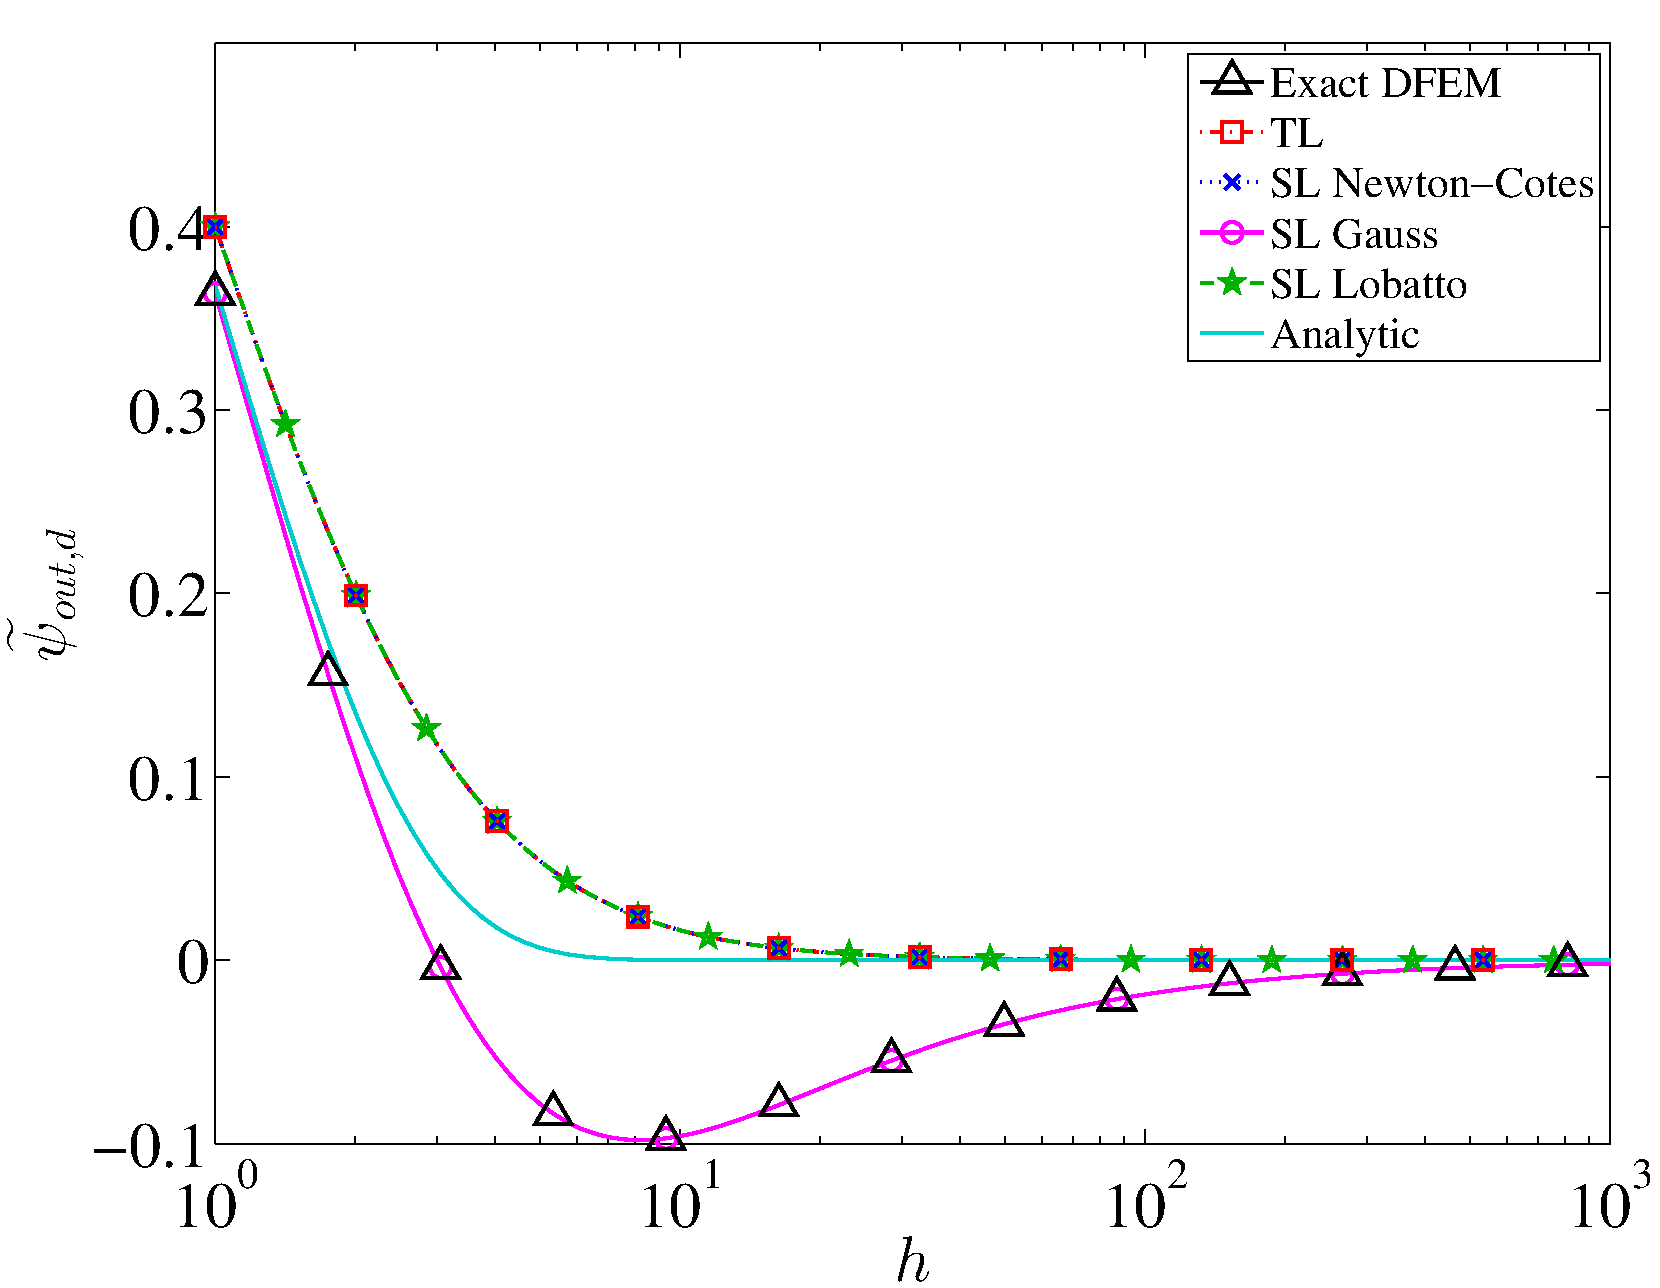
\includegraphics[width=11cm]{chapter2_constant_xs/P1_Outflow_AllMeth-eps-converted-to.pdf}
\caption{Numerical outflow values  as a function of $h$, for a single cell homogeneous absorber problem with a linear DFEM trial space.}
\label{fig:p1_outflow}
\end{figure}
\begin{figure}[!hbp]
\centering
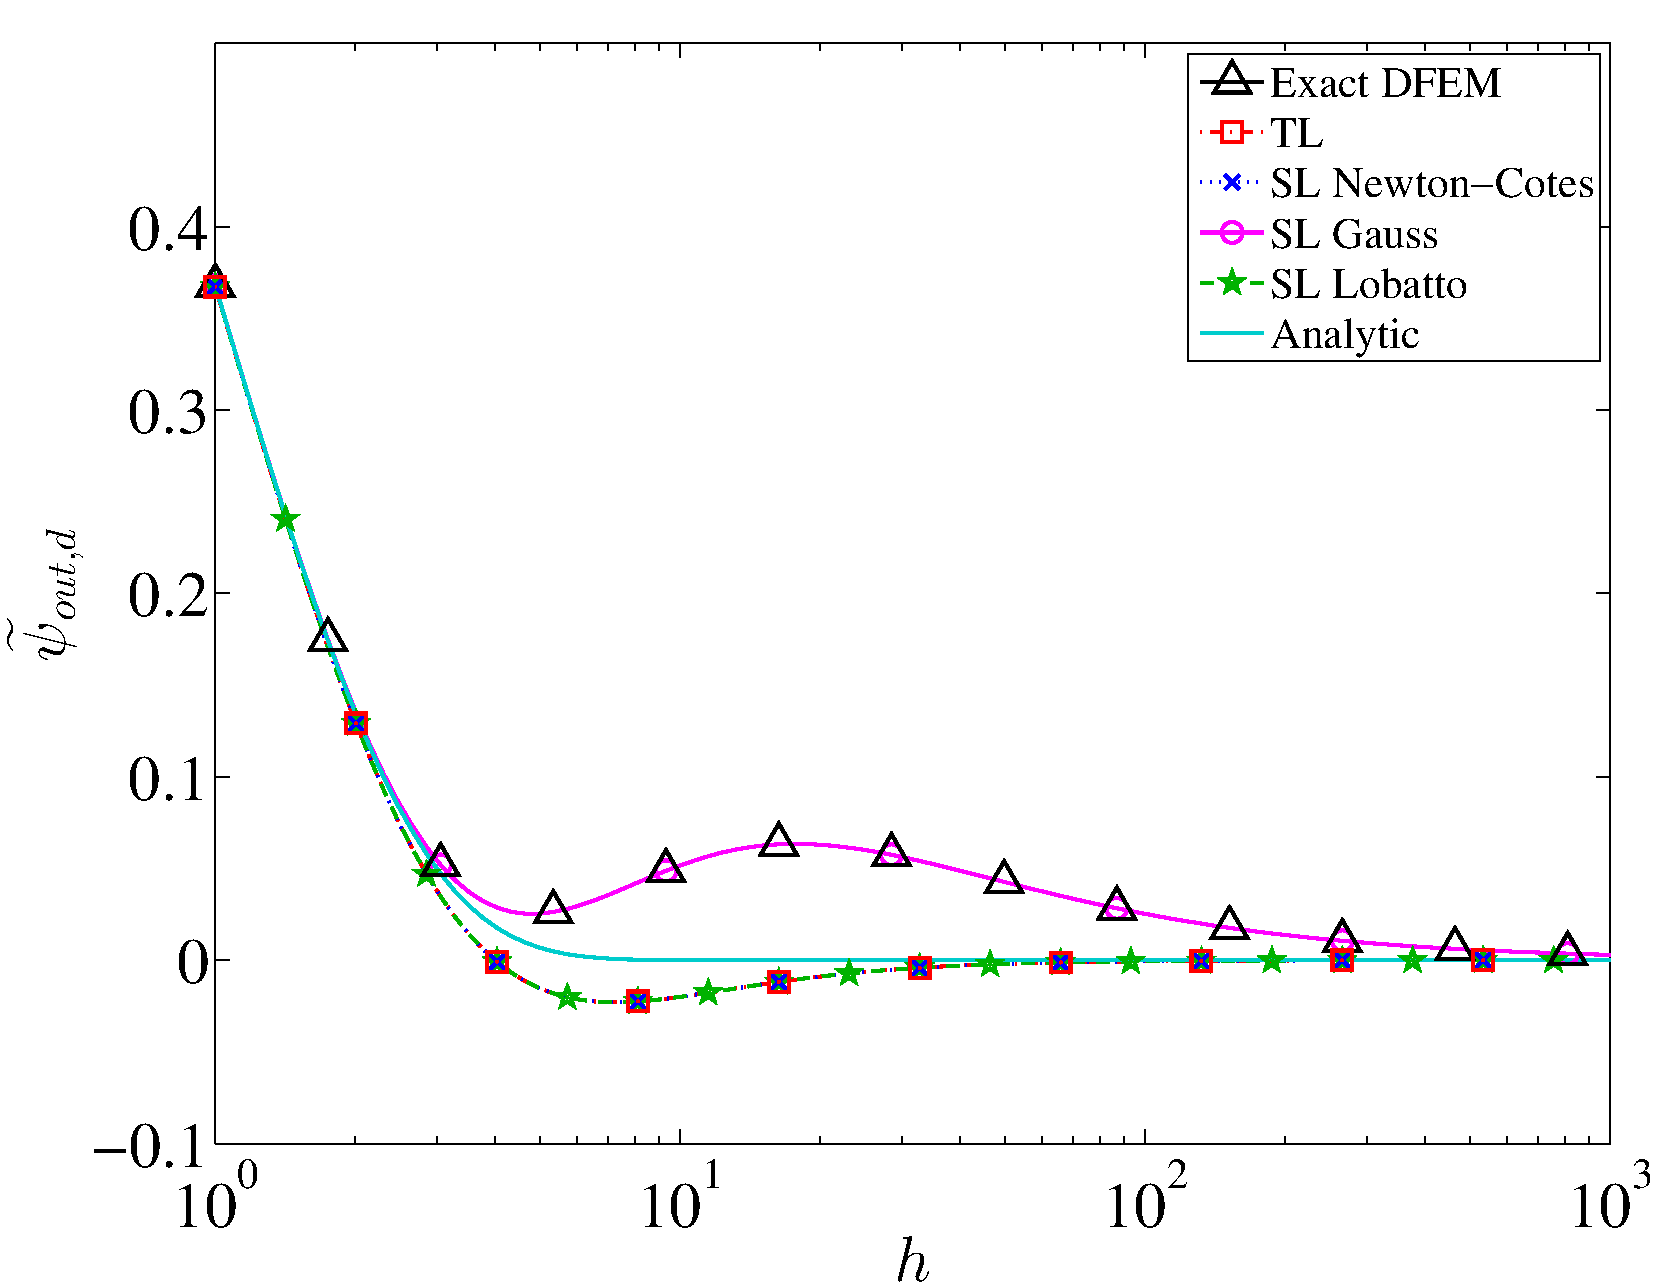
\includegraphics[width=11cm]{chapter2_constant_xs/P2_Outflow_AllMeth-eps-converted-to.pdf}
\caption{Numerical outflow values  as a function of $h$, for a single cell homogeneous absorber problem with a quadratic DFEM trial space.}
\label{fig:p2_outflow}
\end{figure}
\begin{figure}[!htp]
\centering
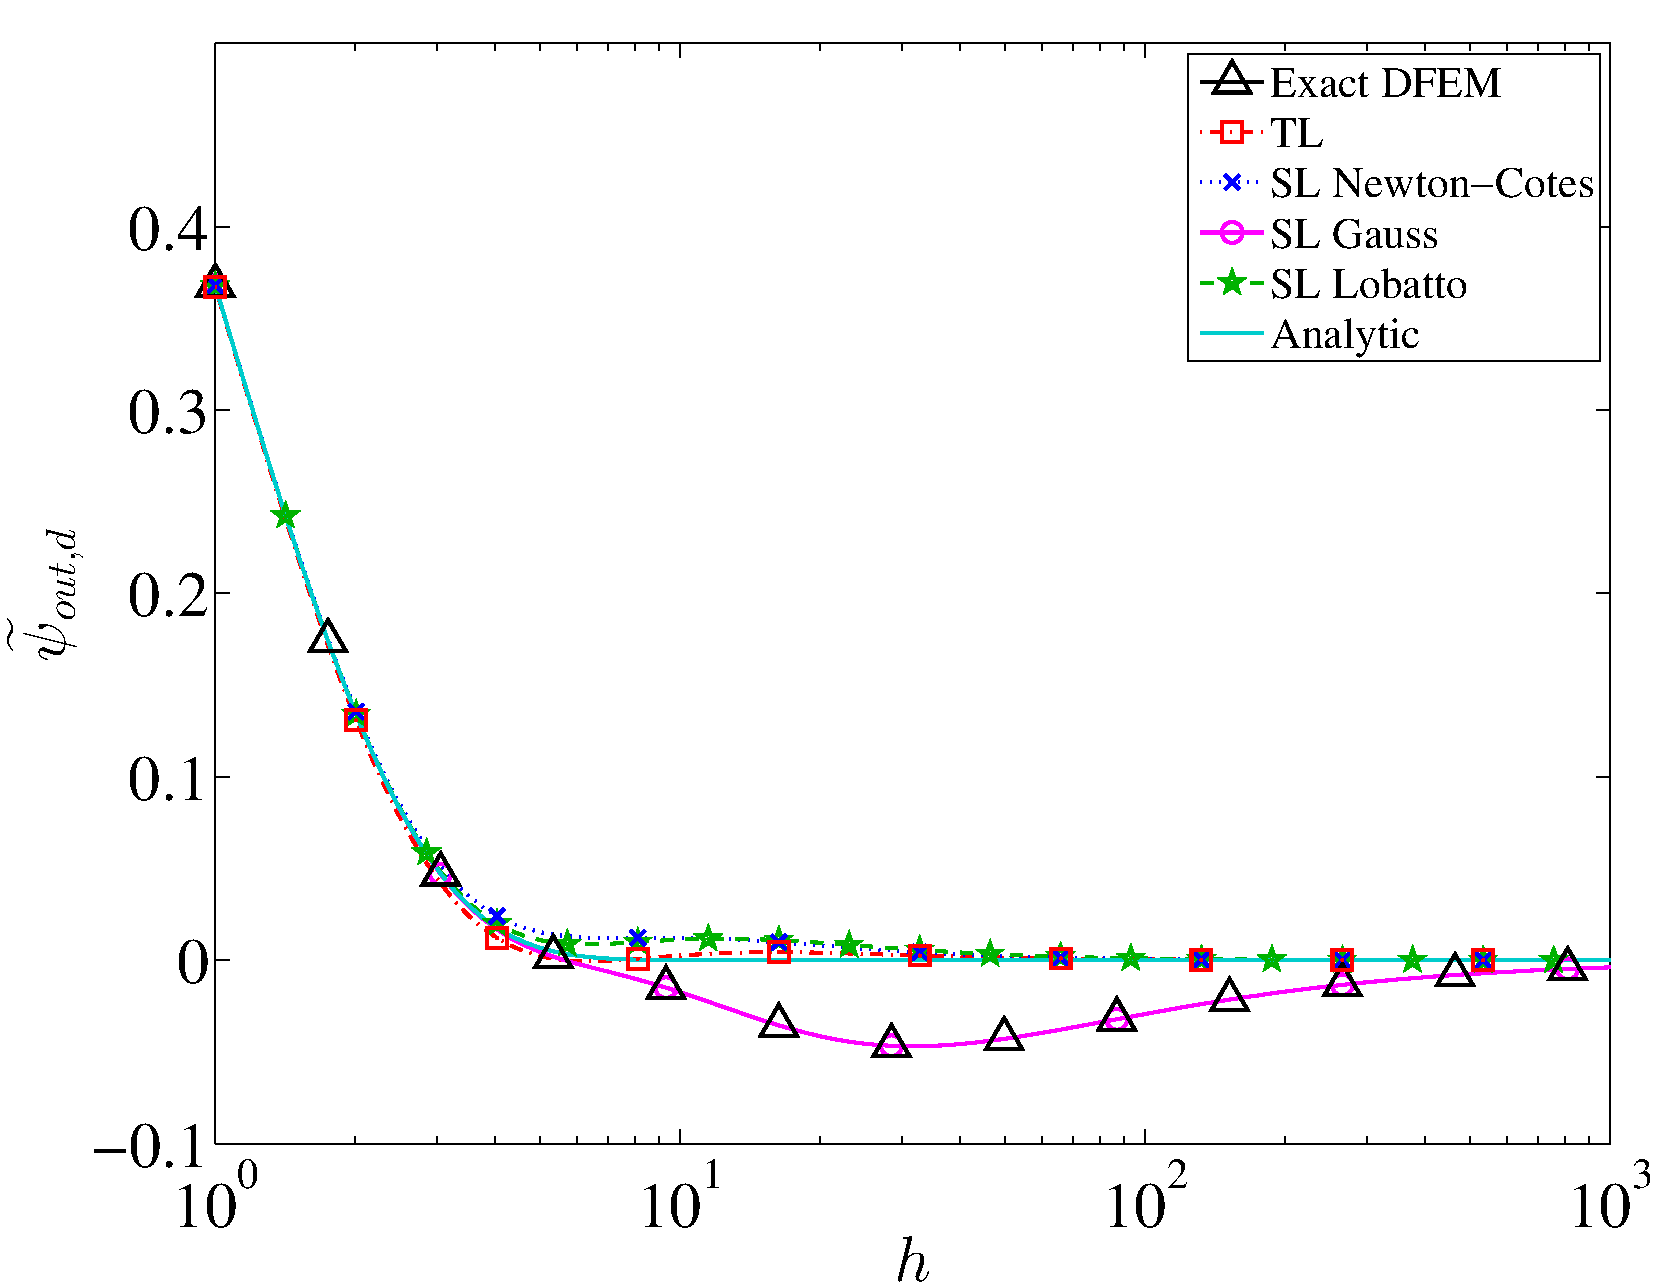
\includegraphics[width=11cm]{chapter2_constant_xs/P3_Outflow_AllMeth-eps-converted-to.pdf}
\caption{Numerical outflow values  as a function of $h$, for a single cell homogeneous absorber problem with a cubic DFEM trial space.}
\label{fig:p3_outflow}
\end{figure}
\begin{figure}[!hbp]
\centering
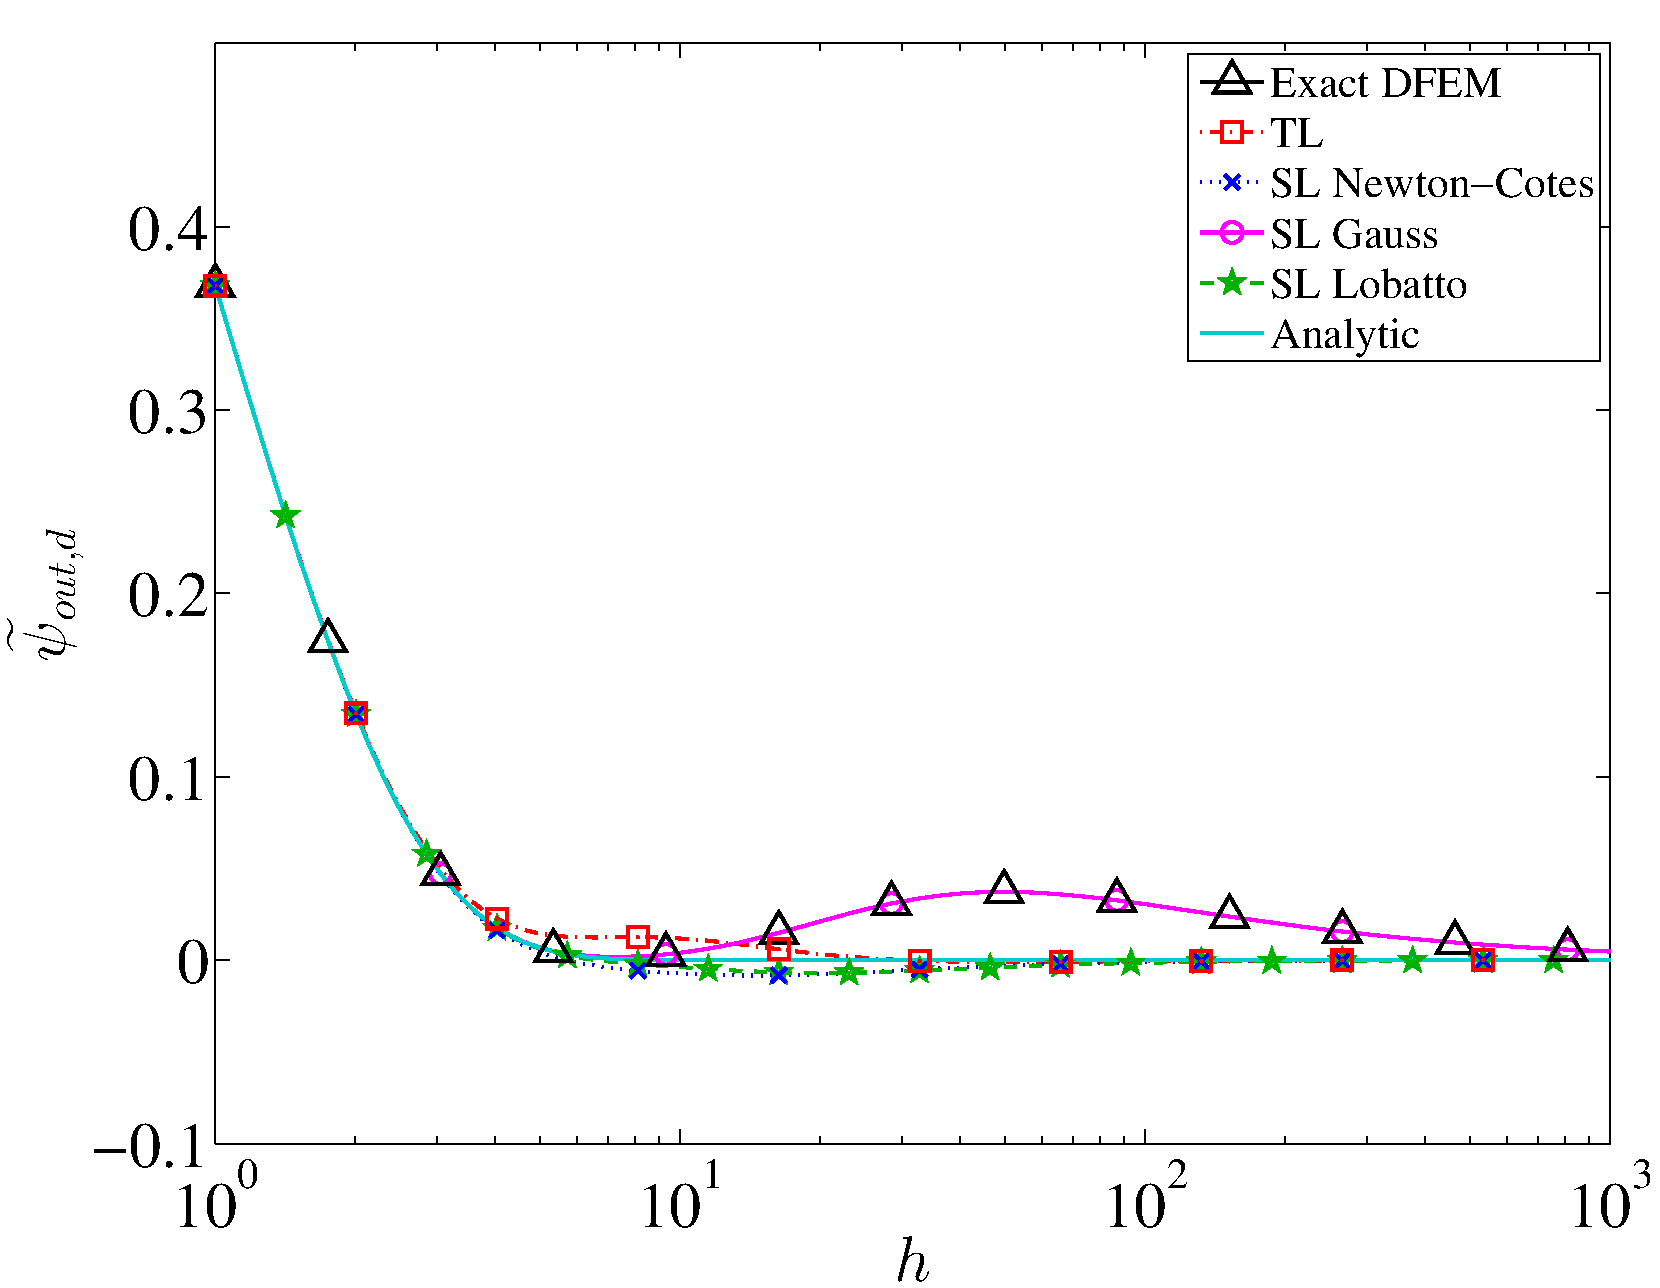
\includegraphics[width=11cm]{chapter2_constant_xs/P4_Outflow_AllMeth-eps-converted-to.pdf}
\caption{Numerical outflow values  as a function of $h$, for a single cell homogeneous absorber problem with a quartic DFEM trial space.}
\label{fig:p4_outflow}
\end{figure}
All methods converge to the analytical solution as $h\to 0$, thus we have zoomed in the range where the methods  visually differ (i.e., $h \ge 1$). 
We observe that:
\begin{itemize}
\item SL Gauss yields strictly positive outflows for even degree polynomial trial spaces,
\item SL Lobatto and SL Newton-Cotes yield strictly positive outflows for odd degree polynomial trial spaces, and
\item TL yields strictly positive outflows only for a linear trial space.
\end{itemize}
We also numerically verify the remarks made of \secref{sec:quad_select}, that is:
\begin{itemize}
\item SL Gauss is equivalent to Exact DFEM,
\item SL Lobatto, SL Newton-Cotes, and TL are equivalent for linear and quadratic trial spaces, and
\item for even degree trial spaces, the outflow value computed by SL Gauss is not monotonically decreasing as a function of $h$ for cells of intermediate optical thickness (the same was noted in \cite{warsa_prinja} for Exact DFEM).
\end{itemize}
%Finally, we note that for even degree polynomial trial spaces, 
%SL Gauss calculates a strictly positive but non-monotonically decreasing value of $\widetilde{\psi}_{out}$ for cells of intermediate optical thickness.
%In addition, Warsa and Prinja also showed that in a source-free pure absorber, a non-physical increase in angular flux outflow occurred in cells of intermediate  optical thickness when using even degree trial spaces.


%%%%%%%%%%%%%%%%%%%%%%%%%%%%%%%%%%%%%%%%%%%%%%%%%%%%%%%%%%%%%%%%%%
\subsection{Fixed Source Single-Cell Inflow Comparison}
\label{sec:inflow}
%%%%%%%%%%%%%%%%%%%%%%%%%%%%%%%%%%%%%%%%%%%%%%%%%%%%%%%%%%%%%%%%%%

As noted in \cite{csz}, it is possible for LDFEM to yield negative solutions near cell inflows for source driven problems.
In this second problem, we use a $\delta$-source:
\benum
Q_d(x) = \left\{ \begin{array}{ll} \delta(x-x_o) & \text{for} ~~ \mu_d > 0 \\ 0  &  \text{for} ~~ \mu_d < 0 \end{array} \right. \pec
\eenum  
$x\in\left[-1,1 \right]$, and $-1 \leq x_o \leq 1$.
The analytic solution to this problem for $\mu_d > 0$ is:
\benum
\psi(x,\mu_d) = \left \{ \begin{array}{ll} \exp\left[-\frac{\Sigma_t(x - x_o)}{\mu_d}  \right] & x \geq x_o \\ 0 & x < x_o \end{array} \right.  \pep
\eenum 
(For $\mu_d < 0$, $\psi(x,\mu_d) = 0$.)
%
We now examine the numerical approximation to the angular flux near the cell inflow, $\widetilde{\psi}_{in,d}$, for various integration 
schemes, trial space degrees, and as a function of the ratio of the first Legendre moment of the source, $S_1$, to the zero-th Legendre moment of the source, $S_0$.
Note that the physical range of that ratio, $\frac{S_1}{S_0}$, is $[-3,3]$, corresponding to a $\delta$-source at the left cell edge $(\frac{S_1}{S_0} = -3)$ or at the right edge $(\frac{S_1}{S_0} = 3)$.

We first consider the case of a vacuum ($\Sigma_t=0$), thus only testing the effect of quadrature accuracy in evaluating $\vec{Q}_d$ and $\mathbf{G}$.  
In \figs{fig:vac_inflow_p1}{fig:vac_inflow_p4}, we plot $\widetilde{\psi}_{in,d}$ for three schemes:
\begin{enumerate}
\item Lobatto quadrature, which is exact for $\mathbf{G}$ and approximate for the source moments, \eqt{eq:mod_source_moment} ,
\item Gauss quadrature: which is exact for both $\mathbf{G}$ and the source moments, and 
\item Newton-Cotes quadrature: which is approximate for both $\mathbf{G}$ and the source moments.
\end{enumerate}
\begin{figure}[!hbp]
\centering
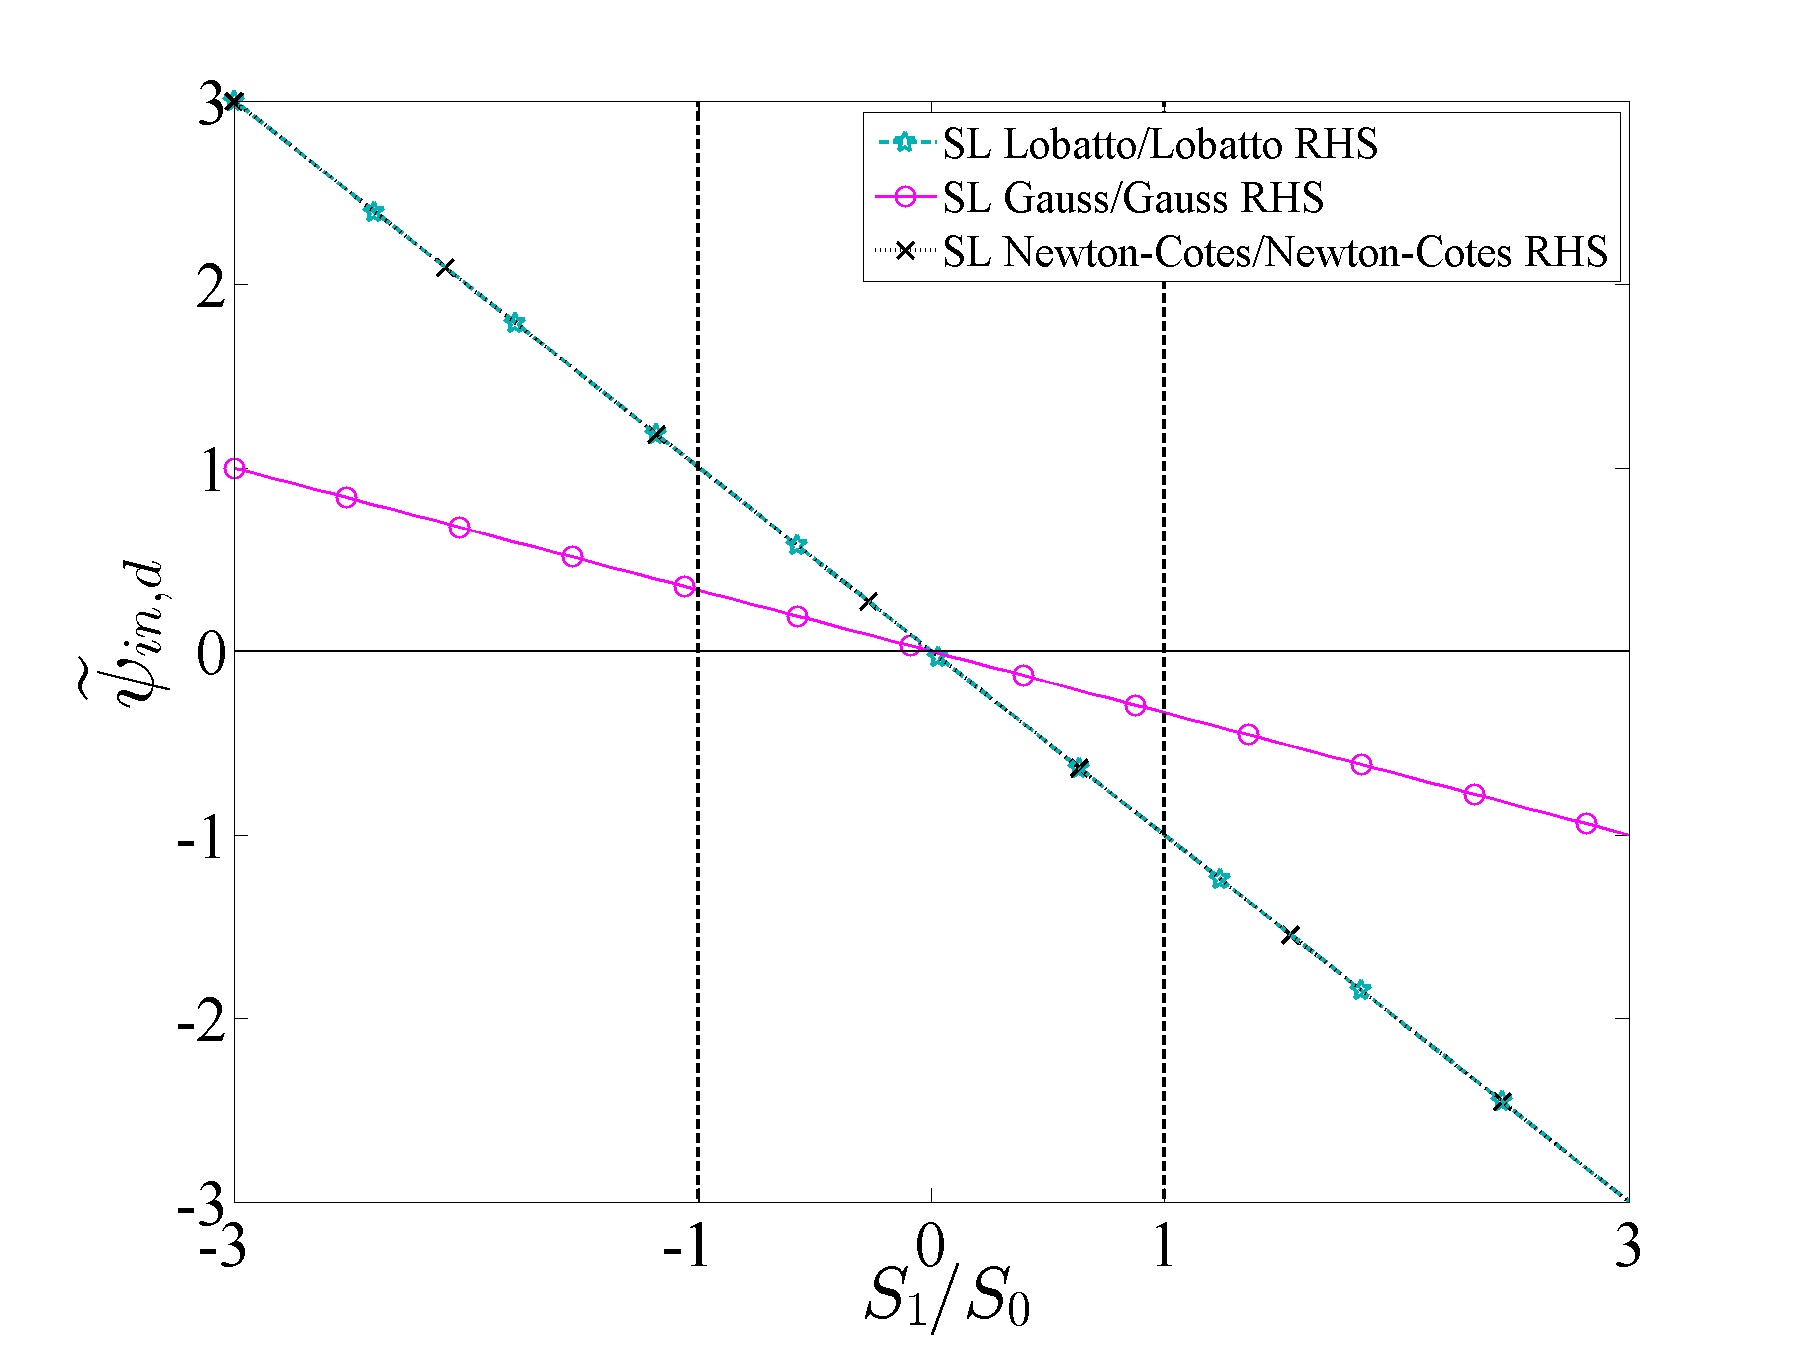
\includegraphics[width=11cm]{chapter2_constant_xs/Final_Inflow_RHS_Comparison_Source_P1_MFP_0.png}
\caption{Numerical inflow values as a function of $\frac{S_1}{S_0}$ for a single cell (vacuum case) with a $\delta$-shaped source, using linear DFEM.}
\label{fig:vac_inflow_p1}
\end{figure}
\begin{figure}[!htp]
\centering
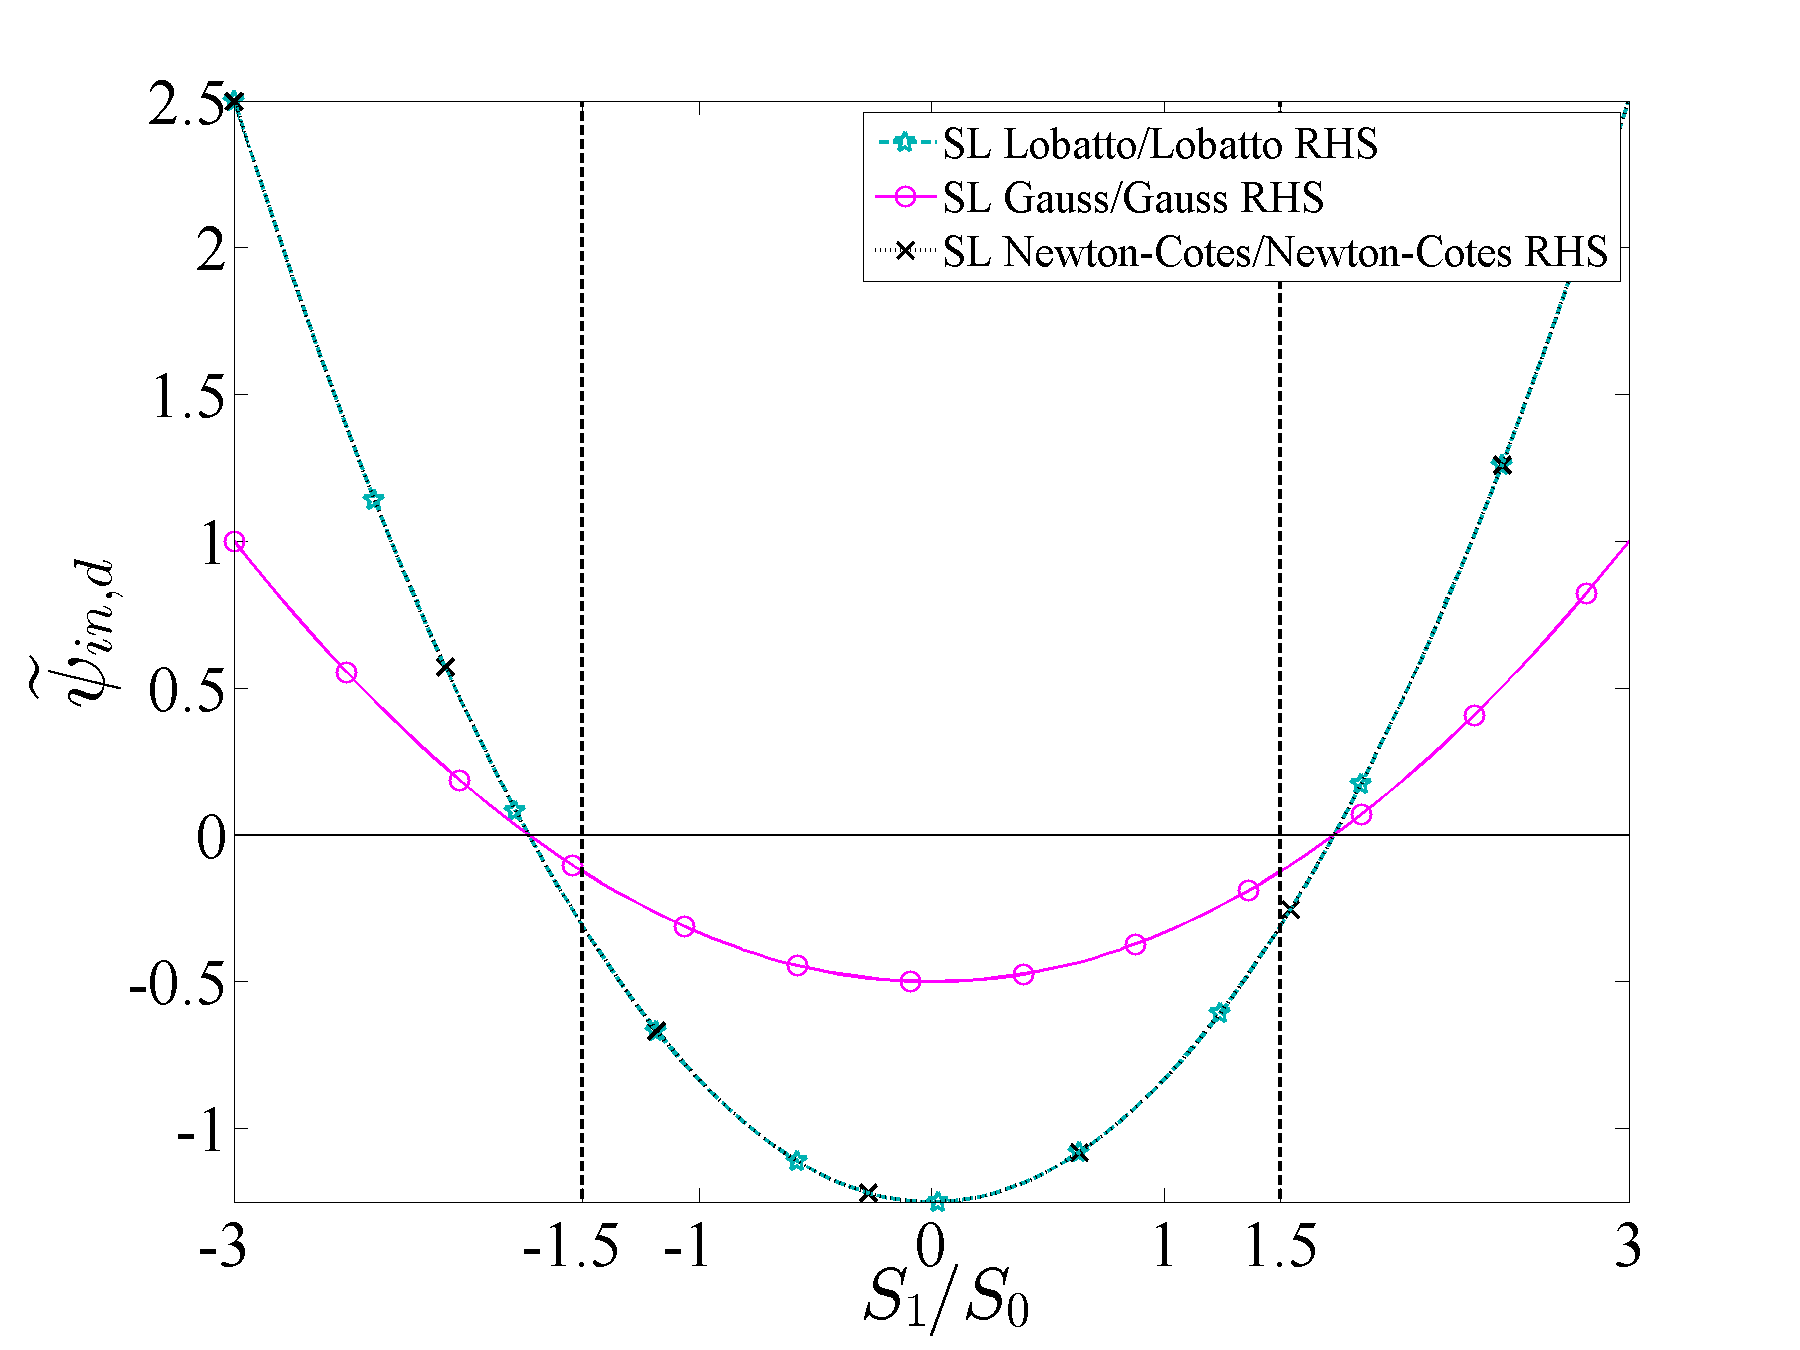
\includegraphics[width=11cm]{chapter2_constant_xs/Final_Inflow_RHS_Comparison_Source_P2_MFP_0.png}
\caption{Numerical inflow values as a function of $\frac{S_1}{S_0}$ for a single cell (vacuum case) with a $\delta$-shaped source, using quadratic DFEM.}
\label{fig:vac_inflow_p2}
\end{figure}
\begin{figure}[!hbp]
\centering
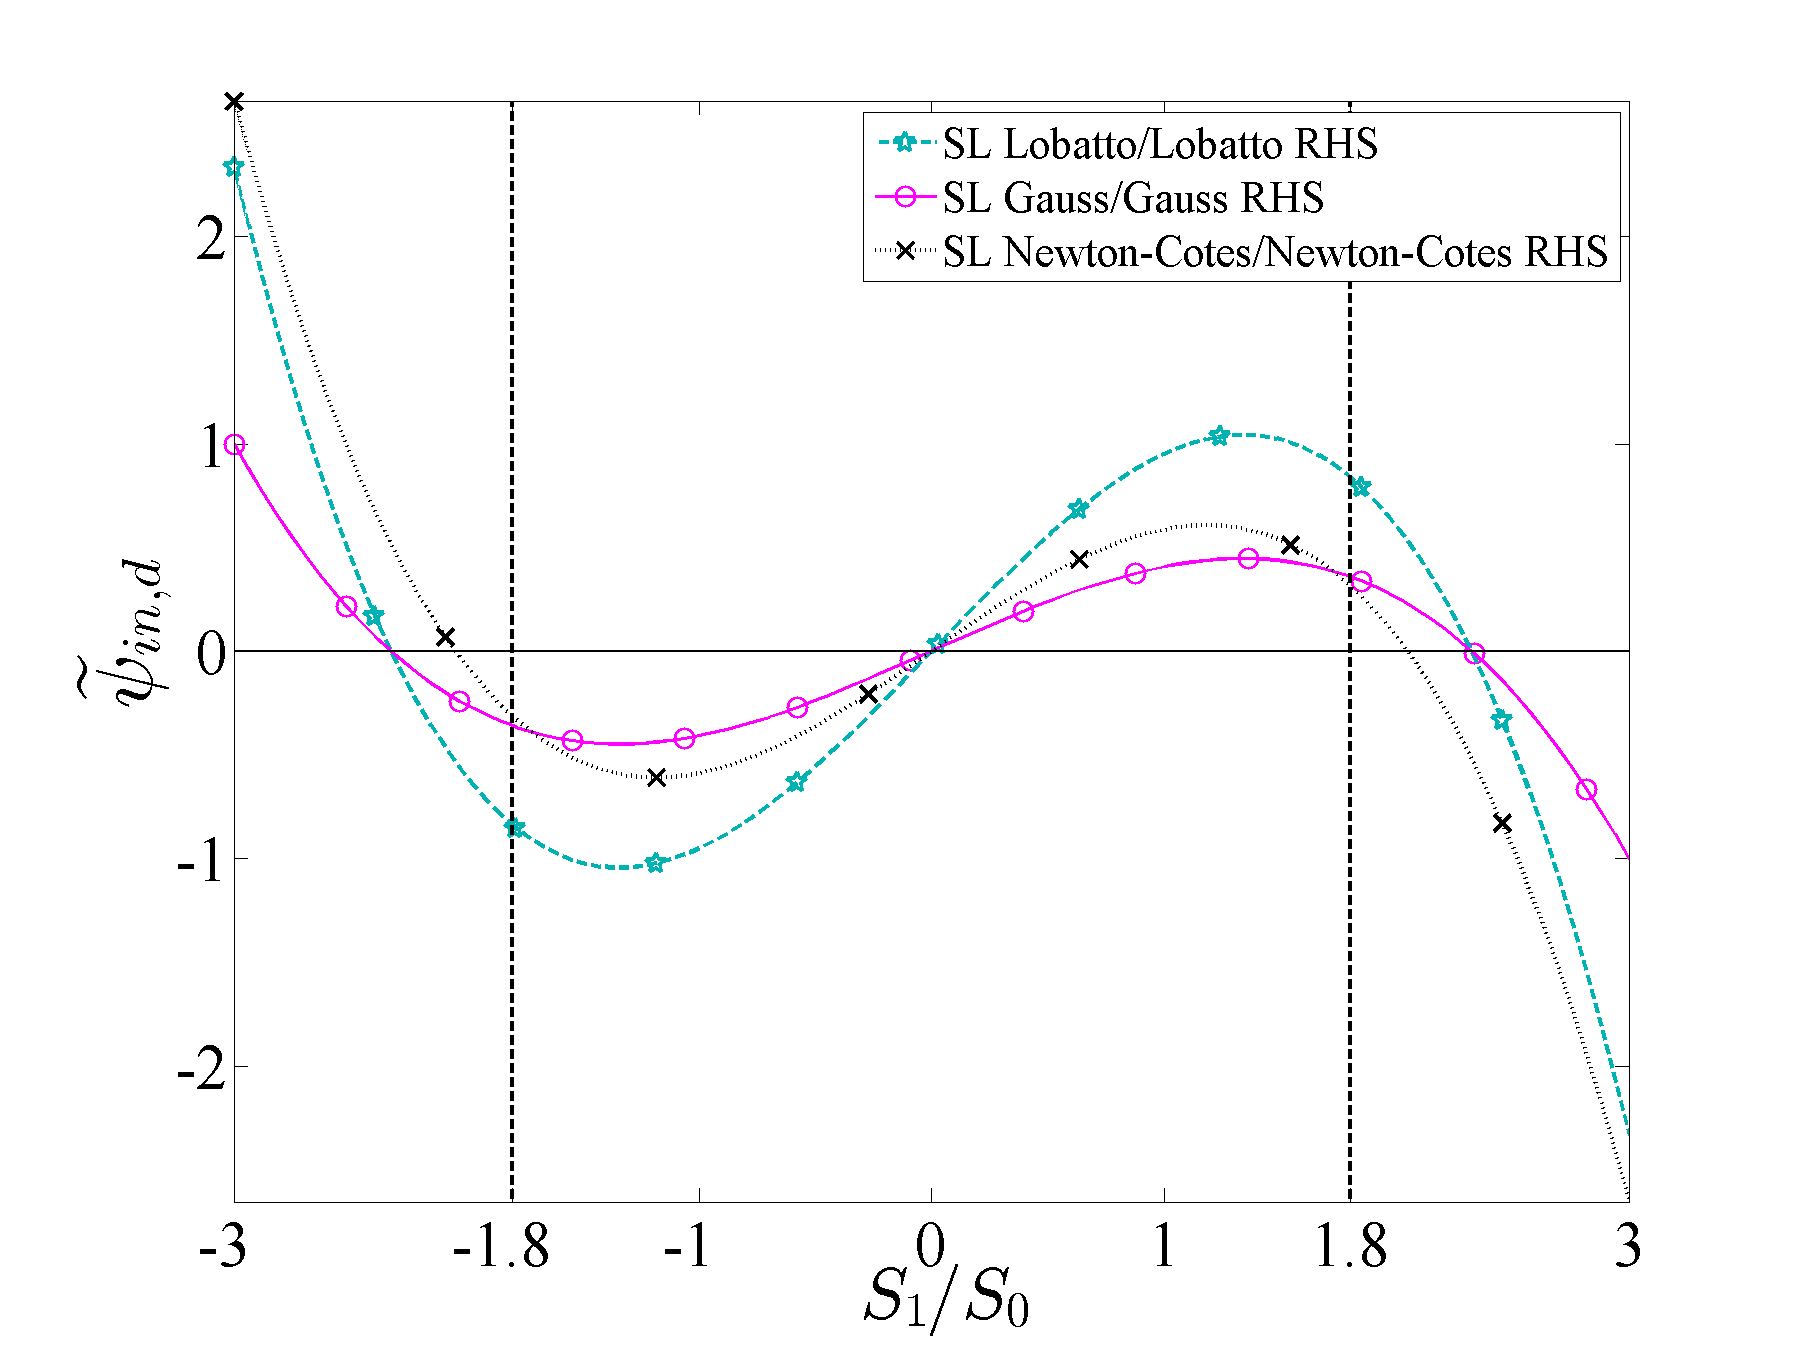
\includegraphics[width=11cm]{chapter2_constant_xs/Final_Inflow_RHS_Comparison_Source_P3_MFP_0.png}
\caption{Numerical inflow values as a function of $\frac{S_1}{S_0}$ for a single cell (vacuum case) with a $\delta$-shaped source, using cubic DFEM.}
\label{fig:vac_inflow_p3}
\end{figure}
\begin{figure}[!htp]
\centering
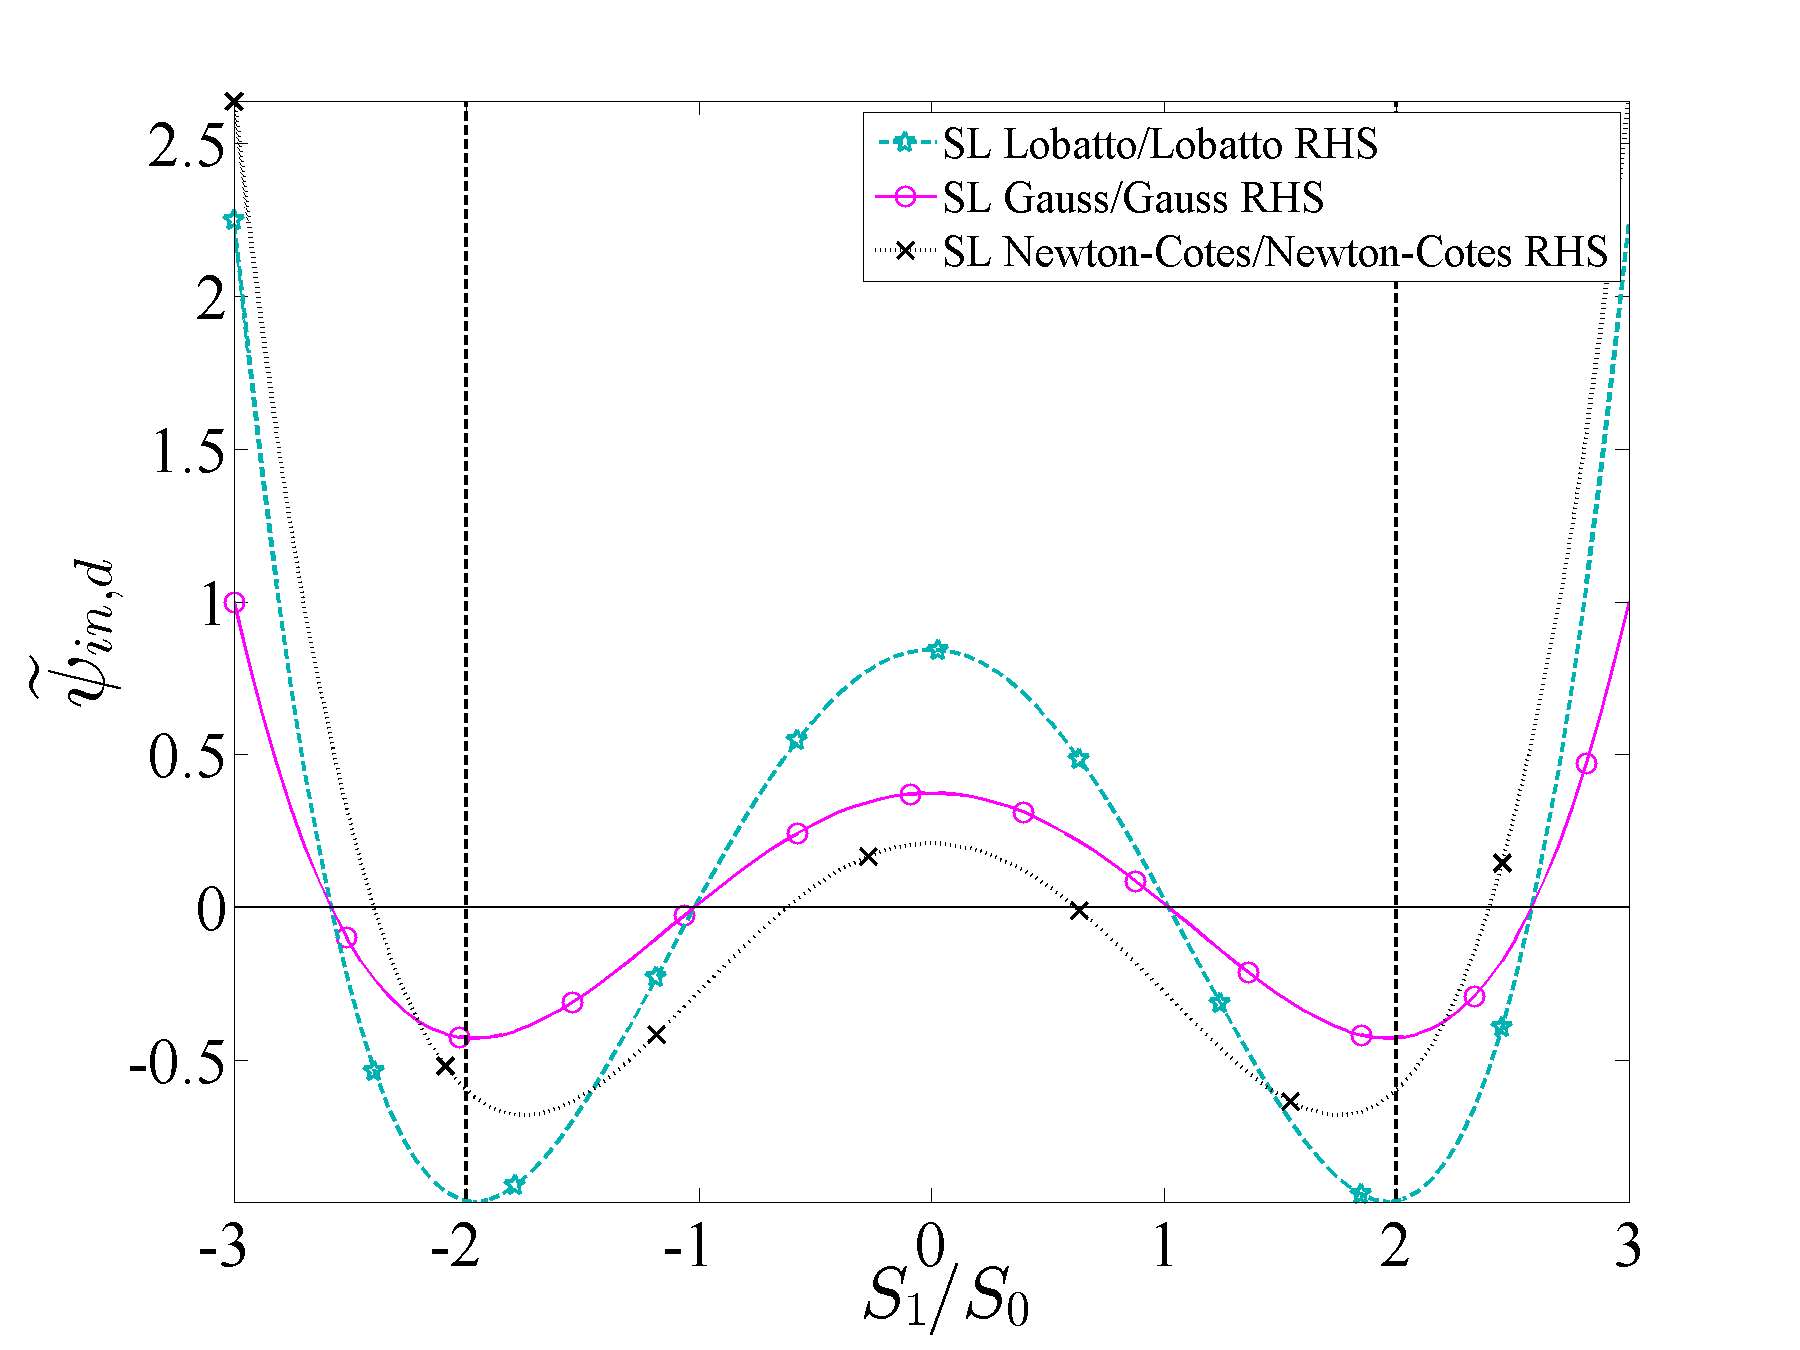
\includegraphics[width=11cm]{chapter2_constant_xs/Final_Inflow_RHS_Comparison_Source_P4_MFP_0.png}
\caption{Numerical inflow values as a function of $\frac{S_1}{S_0}$ for a single cell (vacuum case) with a $\delta$-shaped source, using quartic DFEM.}
\label{fig:vac_inflow_p4}
\end{figure}

The dotted vertical lines in \figs{fig:vac_inflow_p1}{fig:vac_inflow_p4} correspond to the extrema values of $\frac{S_1}{S_0}$ that yield a strictly positive polynomial source representation of degree $P$ 
(indeed, the degree-$P$ Legendre expansion of the $\delta$-source is not everywhere positive for a wide range of possible $\frac{S_1}{S_0}$ that are physically realizable).
For all trial space degrees, the Gauss scheme exhibits less negativity than either of the other two schemes.
The dramatic difference between the Gauss scheme and the Lobatto scheme is solely due to the quadrature formula used to evaluate $\vec{Q}_d$ since both schemes exactly integrate $\mathbf{G}$.
The Newton-Cotes scheme exhibits less severe negativities than the Lobatto scheme but is less robust than the Gauss scheme.
Given the results shown in \figs{fig:vac_inflow_p1}{fig:vac_inflow_p4}, we conclude that the most robust schemes exactly integrate the source moments, \eqt{eq:mod_source_moment}.

\begin{figure}[!htp]
\centering
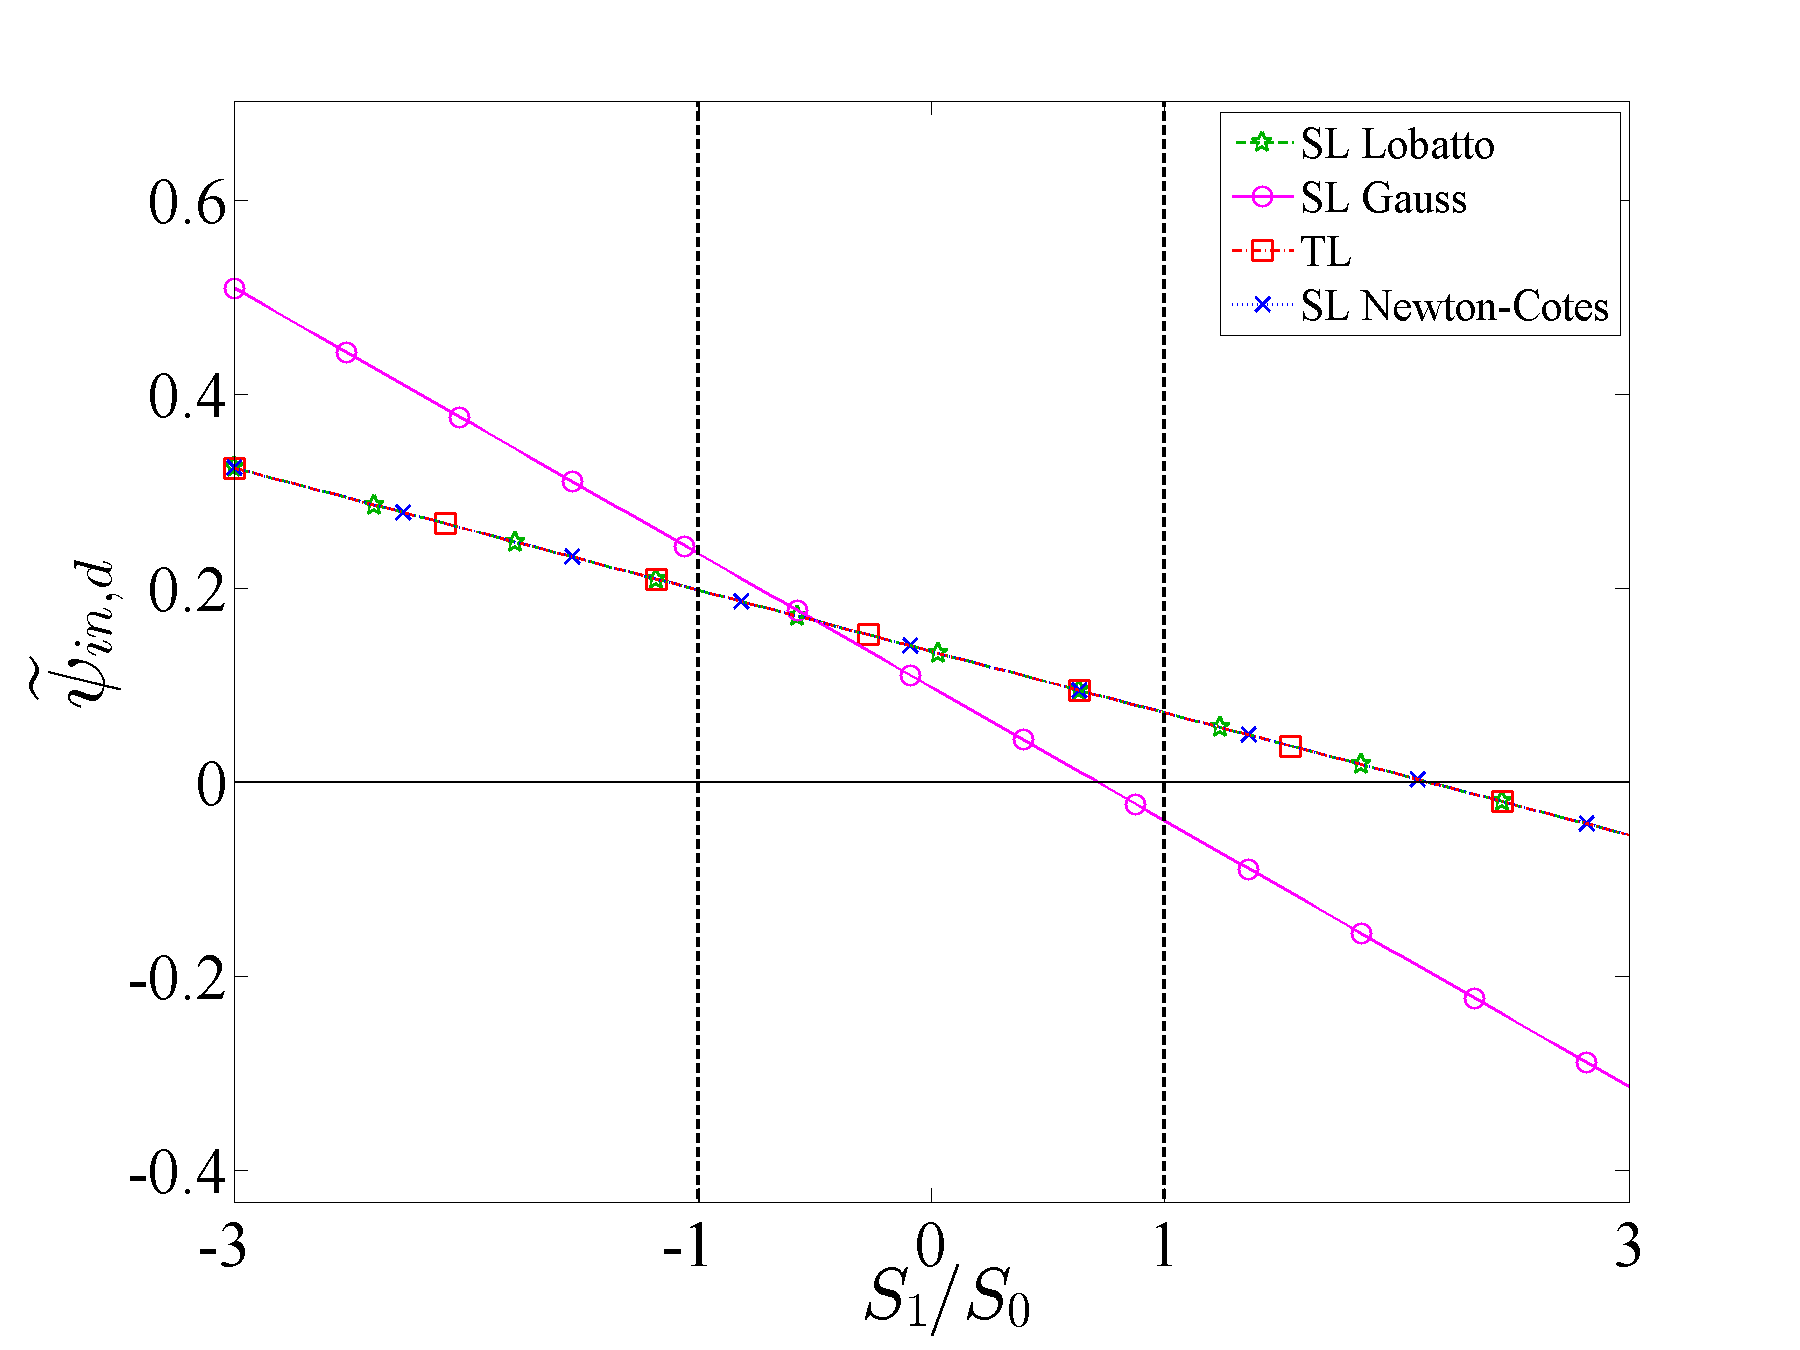
\includegraphics[width=11cm]{chapter2_constant_xs/Final_Inflow_RHS_Comparison_Source_P1_MFP_5.png}
\caption{Numerical inflow values  as a function of $\frac{S_1}{S_0}$, for a single cell (absorber case) with a $\delta$-shaped source, using linear DFEM.}
\label{fig:abs_inflow_p1}
\end{figure}
\begin{figure}[!hbp]
\centering
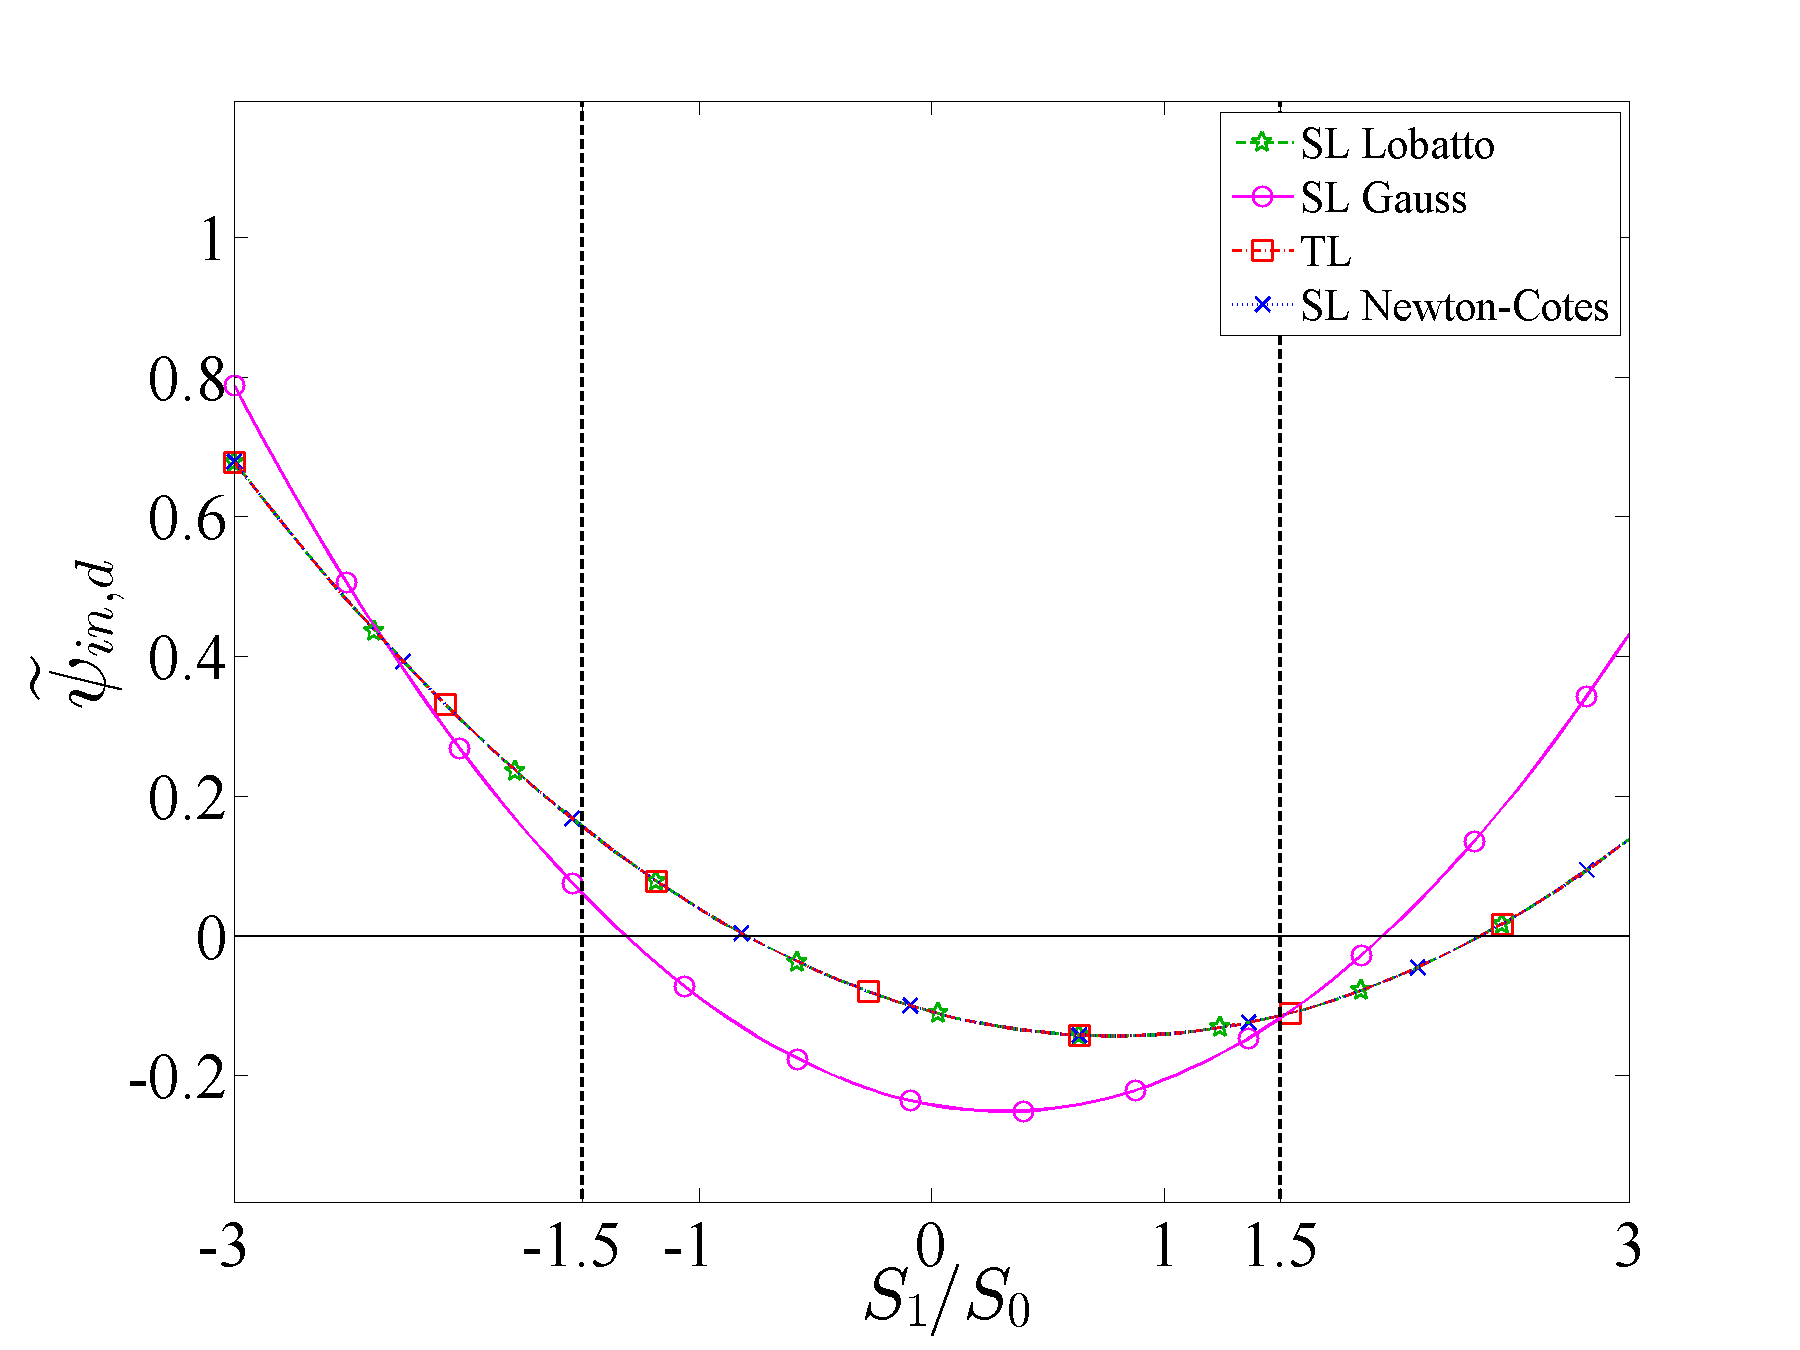
\includegraphics[width=11cm]{chapter2_constant_xs/Final_Inflow_RHS_Comparison_Source_P2_MFP_5.png}
\caption{Numerical inflow values  as a function of $\frac{S_1}{S_0}$, for a single cell (absorber case) with a $\delta$-shaped source, using quadratic DFEM.}
\label{fig:abs_inflow_p2}
\end{figure}
\begin{figure}[!hbp]
\centering
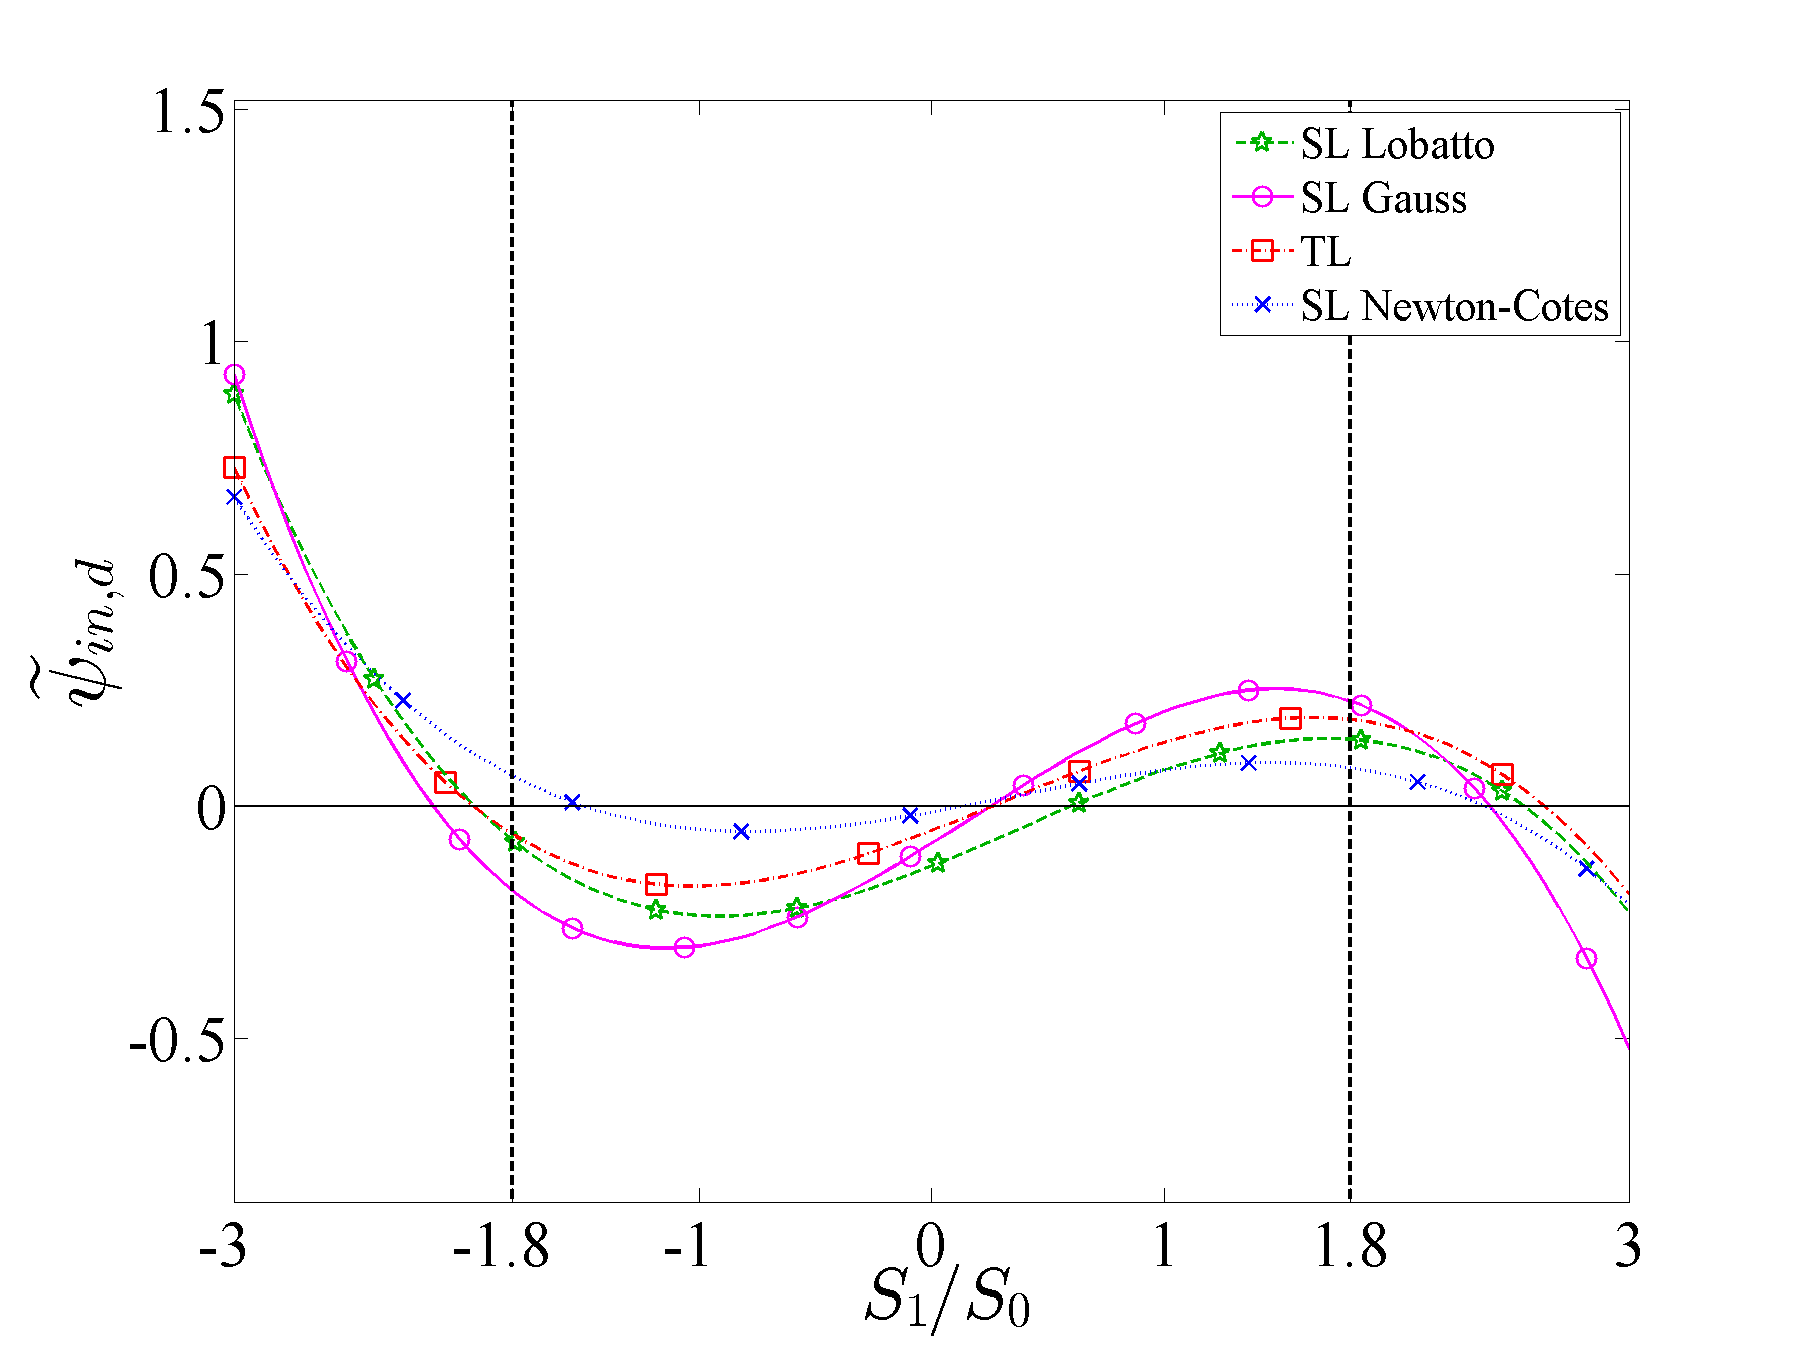
\includegraphics[width=11cm]{chapter2_constant_xs/Final_Inflow_RHS_Comparison_Source_P3_MFP_5.png}
\caption{Numerical inflow values  as a function of $\frac{S_1}{S_0}$, for a single cell (absorber case) with a $\delta$-shaped source, using cubic DFEM.}
\label{fig:abs_inflow_p3}
\end{figure}
\begin{figure}[!htp]
\centering
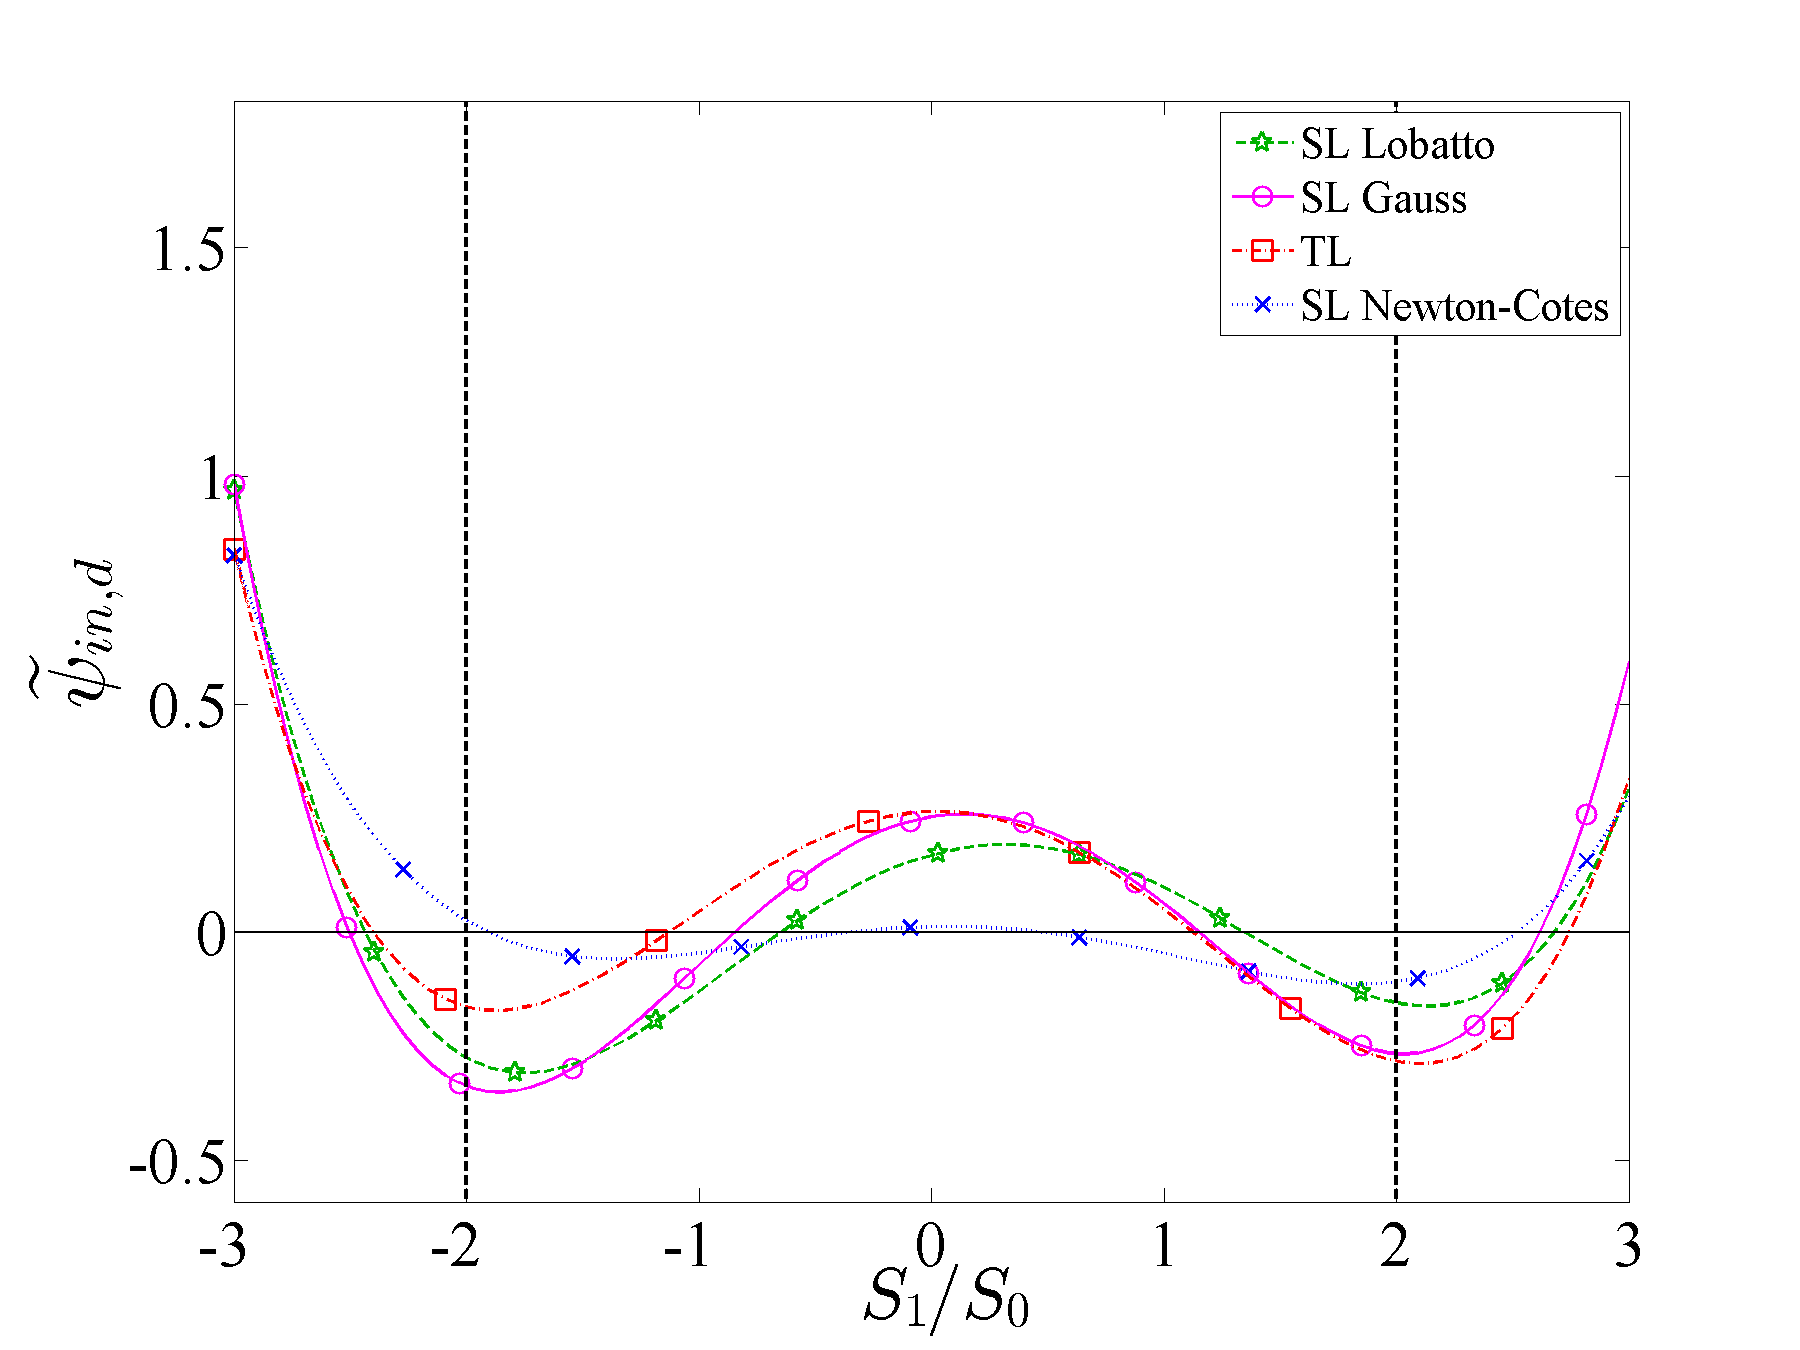
\includegraphics[width=11cm]{chapter2_constant_xs/Final_Inflow_RHS_Comparison_Source_P4_MFP_5.png}
\caption{Numerical inflow values  as a function of $\frac{S_1}{S_0}$, for a single cell (absorber case) with a $\delta$-shaped source, using quartic DFEM.}
\label{fig:abs_inflow_p4}
\end{figure}
\newpage
In \figs{fig:abs_inflow_p1}{fig:abs_inflow_p4}, we again examine the positivity of $\widetilde{\psi}_{in,d}$, but for a non-vacuum case.
Total cell optical thickness was chosen to be 5 mean free paths in \figs{fig:abs_inflow_p1}{fig:abs_inflow_p4} because this value led to the clearest plots.
The relative behaviors observed do not change with cell optical thickness, but using a thicker domain reduces the magnitude for the values of $\widetilde{\psi}_{in,d}$.
All methods in \figs{fig:abs_inflow_p1}{fig:abs_inflow_p4} exactly integrate \eqt{eq:mod_source_moment}.
%, and the scheme naming notation is consistent with \tbl{tbl:names}.
Regardless of trial space chosen,  all schemes exhibit some negativities, but the SL Gauss scheme exhibits the greatest negativities and oscillations. 
The SL Newton-Cotes scheme presents the least severe negativities.


%%%%%%%%%%%%%%%%%%%%%%%%%%%%%%%%%%%%%%%%%%%%%%%%%%%%%%%%%%%%%%%%%%
\subsection{Single-Cell Taylor Series Analysis}
%%%%%%%%%%%%%%%%%%%%%%%%%%%%%%%%%%%%%%%%%%%%%%%%%%%%%%%%%%%%%%%%%%

Next, we perform a local truncation error analysis by comparing the Taylor series expansions for the exact and 
numerical angular fluxes as a function of powers of $h$ for the source-free, incident flux pure absorber problem.  
Matlab \cite{matlab} has been employed to perform the symbolic Taylor series expansions about $h=0$. 
We denote the Taylor-expanded quantities using the subscript $T$. 
The expansions for the analytical inflow, cell average, and outflow are given below:
\begin{subequations}
\label{eq:taylor_ex}
\beanum
\psi_{in,d,T}  &=& \psi_{in,d} \\
\psi_{A,d,T}   &=& \psi_{in,d}\left(1 - \frac{h}{2} + \frac{h^2}{6} - \frac{h^3}{24} + \frac{h^4}{120} - \frac{h^5}{720} \dots     \right)    \\
\psi_{out,d,T} &=& \psi_{in,d}\left(1 - h + \frac{h^2}{2} -\frac{h^3}{6} + \frac{h^4}{24} - \frac{h^5}{120} \dots \right) \pep
\eeanum
\end{subequations}

The Taylor expansions of the numerical analogues to the quantities in \eqts{eq:taylor_ex} depend on the trial space polynomial degree, the choice of interpolatory points, and the numerical integration strategy. 
For brevity, we omit giving these numerical analogues.
Table \ref{tbl:taylor_in_part1} gives the lowest order term for the difference between  $\psi_{in,d,T}$ and the numerical analogs
for the Exact DFEM and TL schemes.  
The same information for the SL Newton-Cotes, SL Gauss, and SL Lobatto schemes is given in \tbl{tbl:taylor_in_part2}.
The differences between $\psi_{A,d,T}$ and the respective numerical analogs are given in \tbl{tbl:taylor_avg_part1} for Exact DFEM and TL,
and \tbl{tbl:taylor_avg_part2} for the SL Newton-Cotes, SL Gauss, and SL Lobatto schemes.
Differences between $\psi{out,d,T}$ and the correseponding numerical analogs are given in \tbl{tbl:taylor_out_part1} for Exact DFEM and TL  and 
\tbl{tbl:taylor_out_part2} gives the lowest order difference between the SL Newton-Cotes, SL Gauss, and SL Lobatto approximations of $\psi_{out,d,T}$.
In Tables \ref{tbl:taylor_in_part1}-\ref{tbl:taylor_out_part2} all entries are listed as
$q(C)$, to be read as ``the difference between the analytic taylor expansion and the numeric analog is $C h^q$ with $h=\Sigma_t \Delta x / \mu$''.
Entries of ``Machine Precision'' in Tables \ref{tbl:taylor_in_part1}-\ref{tbl:taylor_out_part2} are meant to indicate that the difference between
the analytic Taylor expansion and Taylor expansion of the numerical approximation was inconclusive due to all coefficients being within machine precision.
% \begin{landscape}
% \begin{table}[!hbp]
% \centering
% \caption{Local truncation error analysis in $\widetilde{\psi}_{in,d}$ for a single cell problem with constant cross section. 
% Values given as $q(C)$ are to be read as $C h^q$ with $h=\Sigma_t \Delta x / \mu$.}
% \begin{tabular}{|c|c|c|c|c|c|} 
% \hline
  % Polynomial 										  & Exact 										&	 TL  										& SL Newton-Cotes 				& SL Gauss 			 						& SL Lobatto  \\
  % Degree  of $\widetilde{\psi}$		&   DFEM										& {}											& {}		 							 		& {}   										&	 {}   \\
	% \hline
				% 1   											&  2 $(2\times 10^{-1})$		& 2 $(5\times 10^{-1})$		&	2 $(5\times 10^{-1})$		&	2 $(2\times 10^{-1})$		&	2 $(5\times 10^{-1})$	\\
		% \hline
				% 2   											&  3  $(2\times 10^{-2})$		&	3 $(4\times 10^{-2})$		& 3 $(4\times 10^{-2})$		&	3  $(2\times 10^{-2})$	&	3 $(4\times 10^{-2})$		\\
		% \hline	
				% 3   											&  4 $(1\times 10^{-3})$		& 2 $(7\times 10^{-2})$		&	2 $(1\times 10^{-1})$		& 4 $(1\times 10^{-3})$		&	4 $(3\times 10^{-3})$	\\
		% \hline
				% 4   											&  5 $(7\times 10^{-5})$		& 3 $(1\times 10^{-2})$		&	3 $(1\times 10^{-2})$		&	5 $(7\times 10^{-5})$		&	5 $(1\times 10^{-4})$	\\
		% \hline	
				% 5   											&  6 $(3\times 10^{-6})$		& 2 $(5\times 10^{-2})$		&	2 $(6\times 10^{-2})$		&	6 $(3\times 10^{-6})$		&	6 $(7\times 10^{-6})$	\\
		% \hline		
				% 6   											&  7 $(1\times 10^{-7})$		& 3 $(1\times 10^{-2})$		&	3 $(9\times 10^{-3})$		&	7 $(1\times 10^{-7})$		&	7 $(3\times 10^{-7})$	\\
		% \hline		
				% 7   											&  8 $(4\times 10^{-9})$		& 2 $(5\times 10^{-2})$		&	2 $(4\times 10^{-2})$		&	8 $(4\times 10^{-9})$		&	8 $(8\times 10^{-9})$	\\
		% \hline		
% \end{tabular}
% \label{tbl:taylor_in} 
% \end{table}
% \end{landscape}
\begin{table}[!hbp]
\centering
\caption{Local truncation error analysis in $\widetilde{\psi}_{in,d}$ for a single cell problem with constant cross section, for Exact DFEM and TL. }
\begin{tabular}{|c|c|c|} 
\hline
  Polynomial 										  & Exact 										&	 TL                   \\
  Degree  of $\widetilde{\psi}$		&   DFEM										& {}	                  \\
	\hline
				1   											&  2 $(2\times 10^{-1})$		& 2 $(5\times 10^{-1})$		\\
		\hline
				2   											&  3  $(2\times 10^{-2})$		&	3 $(4\times 10^{-2})$	\\
		\hline	
				3   											&  4 $(1\times 10^{-3})$		& 2 $(7\times 10^{-2})$	\\
		\hline
				4   											&  5 $(7\times 10^{-5})$		& 3 $(1\times 10^{-2})$	\\
		\hline	
				5   											&  6 $(3\times 10^{-6})$		& 2 $(5\times 10^{-2})$	\\
		\hline		
				6   											&  7 $(1\times 10^{-7})$		& 3 $(1\times 10^{-2})$	\\
		\hline		
				7   											&  8 $(4\times 10^{-9})$		& 2 $(5\times 10^{-2})$	\\
		\hline		
\end{tabular}
\label{tbl:taylor_in_part1} 
\end{table}
\begin{table}[!htp]
\centering
\caption{Local truncation error analysis in $\widetilde{\psi}_{in,d}$ for a single cell problem with constant cross section, for SL Newton-Cotes, SL Gauss, and SL Lobatto. }
\begin{tabular}{|c|c|c|c|} 
\hline
  Polynomial 										 & SL Newton-Cotes 				& SL Gauss 			 						& SL Lobatto  \\
  Degree  of $\widetilde{\psi}$	& {}		 							 		& {}   										&	 {}   \\
	\hline
				1   										&	2 $(5\times 10^{-1})$		&	2 $(2\times 10^{-1})$		&	2 $(5\times 10^{-1})$	\\
		\hline
				2   										& 3 $(4\times 10^{-2})$		&	3  $(2\times 10^{-2})$	&	3 $(4\times 10^{-2})$		\\
		\hline	
				3   										&	2 $(1\times 10^{-1})$		& 4 $(1\times 10^{-3})$		&	4 $(3\times 10^{-3})$	\\
		\hline
				4   										&	3 $(1\times 10^{-2})$		&	5 $(7\times 10^{-5})$		&	5 $(1\times 10^{-4})$	\\
		\hline	
				5   										&	2 $(6\times 10^{-2})$		&	6 $(3\times 10^{-6})$		&	6 $(7\times 10^{-6})$	\\
		\hline		
				6   										&	3 $(9\times 10^{-3})$		&	7 $(1\times 10^{-7})$		&	7 $(3\times 10^{-7})$	\\
		\hline		
				7   										&	2 $(4\times 10^{-2})$		&	8 $(4\times 10^{-9})$		&	8 $(8\times 10^{-9})$	\\
		\hline		
\end{tabular}
\label{tbl:taylor_in_part2} 
\end{table}
%
%
% \begin{table}[!htp]
% \centering
% \caption{Local truncation error analysis in $\widetilde{\psi}_{A,d}$ for a single cell problem with constant cross section, for Exact DFEM and TL.}
% \begin{tabular}{|c|c|c|c|c|c|} 
% \hline
  % Polynomial 										  & Exact 											& TL  										& SL Newton-Cotes 					& SL Gauss 			 						& SL Lobatto  \\
  % Degree  of $\widetilde{\psi}$		&   DFEM											& {}											& {}		 							 			& {}   											&	 {}   \\
  	% \hline
				% 1   											&  	3 $(1\times 10^{-2})$			& 2 $(2\times 10^{-1})$		&	2 $(2\times 10^{-1})$			&	3 $(1\times 10^{-2})$			&	2 $(2\times 10^{-1})$		\\
		% \hline
				% 2   											&   5 $(1\times 10^{-4})$			&  4 $(2\times 10^{-3})$	&	4 $(2\times 10^{-3})$			&	5 $(1\times 10^{-4})$			&	4 $(2\times 10^{-3})$		\\
		% \hline	
				% 3   											&   7 $(7\times 10^{-7})$			& 3 $(3\times 10^{-3})$		&	4 $(6\times 10^{-4})$			&	 7 $(7\times 10^{-7})$		&	6 $(1\times 10^{-5})$\\
		% \hline
				% 4   											&  9 $(2\times 10^{-9})$			& 5 $(8\times 10^{-5})$		&	6 $(8\times 10^{-6})$			&	9 $(2\times 10^{-9})$			&	8 $(5\times 10^{-8})$	\\
		% \hline
				% 5   											&  11 $(5\times 10^{-12})$		& 3 $(1\times 10^{-3})$		&	6 $(2\times 10^{-6})$			&	11 $(5\times 10^{-12})$		&	10 $(1\times 10^{-10})$\\
		% \hline	
				% 6   											&  13 $(7\times 10^{-15})$		& 5 $(7\times 10^{-5})$		&	8 $(2\times 10^{-8})$			&	13 $(7\times 10^{-15})$		&	12 $(2\times 10^{-13})$\\
		% \hline
				% 7   											&  Machine Precision					& 3 $(1\times 10^{-3})$		&	8 $(3\times 10^{-9})$			&	Machine Precision					&	Machine Precision   \\
		% \hline	
% \end{tabular}
% \label{tbl:taylor_avg} 
% \end{table}
% \end{landscape}
% \pagebreak
% \begin{landscape}
% \begin{table}[!hbp]
% \centering
% \caption{Local truncation error analysis in $\widetilde{\psi}_{out,d}$ for a single cell with constant cross section, for SL Newton-Cotes, SL Gauss, and SL Lobatto.}
% \begin{tabular}{|c|c|c|c|c|c|} 
% \hline
  % Polynomial 										  & Exact 										& TL  										& SL Newton-Cotes 					& SL Gauss 			 					& SL Lobatto  \\
  % Degree  of $\widetilde{\psi}$		&   DFEM										& {}											& {}		 							 			& {}   										&	 {}   \\
  	% \hline
				% 1   											&  4 $(1\times 10^{-2})$		& 3 $(2\times 10^{-1})$		&	3 $(2\times 10^{-1})$		&	4 $(1\times 10^{-2})$			&	3 $(2\times 10^{-1})$	\\
		% \hline
				% 2   											&  6 $(1\times 10^{-4})$		& 5 $(2\times 10^{-3})$		&	5 $(2\times 10^{-3})$			&	6 $(1\times 10^{-4})$		&	5 $(2\times 10^{-3})$		\\
		% \hline	
				% 3   											&  8 $(7\times 10^{-7})$		& 4 $(3\times 10^{-3})$		&	5 $(6\times 10^{-4})$		&	8 $(7\times 10^{-7})$			&	7 $(1\times 10^{-5})$	\\
		% \hline
				% 4   											&  10 $(2\times 10^{-9})$		& 6 $(1\times 10^{-2})$		&	7 $(8\times 10^{-6})$		&	10 $(2\times 10^{-9})$		&	9 $(5\times 10^{-8})$	\\
		% \hline
				% 5   											&  12 $(5\times 10^{-12})$	& 4 $(1\times 10^{-3})$		&	7 $(2\times 10^{-6})$		&	12 $(5\times 10^{-12})$		&	11 $(1\times 10^{-10})$	\\
		% \hline		
				% 6   											&  14 $(7\times 10^{-15})$	& 6 $(7\times 10^{-5})$		&	9 $(2\times 10^{-8})$		&	14 $(7\times 10^{-15})$		&	13 $(2\times 10^{-13})$\\
		% \hline
				% 7   											&  Machine Precision				& 4 $(1\times 10^{-3})$		&	9 $(3\times 10^{-9})$		& Machine Precision					&	Machine Precision  \\
		% \hline
% \end{tabular}
% \label{tbl:taylor_out} 
% \end{table}
% \end{landscape}
\begin{table}[!htp]
\centering
\caption{Local truncation error analysis in $\widetilde{\psi}_{A,d}$ for a single cell problem with constant cross section, for Exact DFEM and TL.}
\begin{tabular}{|c|c|c||} 
\hline
  Polynomial 										  & Exact 											& TL   \\
  Degree  of $\widetilde{\psi}$		&   DFEM											& {}	 \\
  	\hline
				1   											&  	3 $(1\times 10^{-2})$			& 2 $(2\times 10^{-1})$		 \\
		\hline
				2   											&   5 $(1\times 10^{-4})$			&  4 $(2\times 10^{-3})$	\\
		\hline	
				3   											&   7 $(7\times 10^{-7})$			& 3 $(3\times 10^{-3})$	\\
		\hline
				4   											&  9 $(2\times 10^{-9})$			& 5 $(8\times 10^{-5})$	\\
		\hline
				5   											&  11 $(5\times 10^{-12})$		& 3 $(1\times 10^{-3})$	\\
		\hline	
				6   											&  13 $(7\times 10^{-15})$		& 5 $(7\times 10^{-5})$	\\
		\hline
				7   											&  Machine Precision					& 3 $(1\times 10^{-3})$  \\
		\hline	
\end{tabular}
\label{tbl:taylor_avg_part1} 
\end{table}
\begin{table}[!hbp]
\centering
\caption{Local truncation error analysis in $\widetilde{\psi}_{A,d}$ for a single cell problem with constant cross section, for SL Newton-Cotes, SL Gauss, and SL Lobatto}
\begin{tabular}{|c|c|c|c|} 
\hline
  Polynomial 										 & SL Newton-Cotes 					& SL Gauss 			 						& SL Lobatto  \\
  Degree  of $\widetilde{\psi}$	  & {}		 							 			& {}   											&	 {}   \\
  	\hline
				1   									  &	2 $(2\times 10^{-1})$			&	3 $(1\times 10^{-2})$			&	2 $(2\times 10^{-1})$		\\
		\hline
				2   							     &	4 $(2\times 10^{-3})$			&	5 $(1\times 10^{-4})$			&	4 $(2\times 10^{-3})$		\\
		\hline	
				3   								  	&	4 $(6\times 10^{-4})$			&	 7 $(7\times 10^{-7})$		&	6 $(1\times 10^{-5})$\\
		\hline
				4   									  &	6 $(8\times 10^{-6})$			&	9 $(2\times 10^{-9})$			&	8 $(5\times 10^{-8})$	\\
		\hline
				5   								  	&	6 $(2\times 10^{-6})$			&	11 $(5\times 10^{-12})$		&	10 $(1\times 10^{-10})$\\
		\hline	
				6   								  	&	8 $(2\times 10^{-8})$			&	13 $(7\times 10^{-15})$		&	12 $(2\times 10^{-13})$\\
		\hline
				7   								  	&	8 $(3\times 10^{-9})$			&	Machine Precision					&	Machine Precision   \\
		\hline	
\end{tabular}
\label{tbl:taylor_avg_part2} 
\end{table}
%
\pagebreak
%
\begin{table}[!htp]
\centering
\caption{Local truncation error analysis in $\widetilde{\psi}_{out,d}$ for a single cell with constant cross section, for Exact DFEM and TL.}
\begin{tabular}{|c|c|c|} 
\hline
  Polynomial 										  & Exact 										& TL  	\\
  Degree  of $\widetilde{\psi}$		&   DFEM										& {}	\\
  	\hline
				1   											&  4 $(1\times 10^{-2})$		& 3 $(2\times 10^{-1})$	\\
		\hline
				2   											&  6 $(1\times 10^{-4})$		& 5 $(2\times 10^{-3})$	\\
		\hline	
				3   											&  8 $(7\times 10^{-7})$		& 4 $(3\times 10^{-3})$	\\
		\hline
				4   											&  10 $(2\times 10^{-9})$		& 6 $(1\times 10^{-2})$	\\
		\hline
				5   											&  12 $(5\times 10^{-12})$	& 4 $(1\times 10^{-3})$	\\
		\hline		
				6   											&  14 $(7\times 10^{-15})$	& 6 $(7\times 10^{-5})$	\\
		\hline
				7   											&  Machine Precision				& 4 $(1\times 10^{-3})$	\\
		\hline
\end{tabular}
\label{tbl:taylor_out_part1} 
\end{table}
%
%
\begin{table}[!htp]
\centering
\caption{Local truncation error analysis in $\widetilde{\psi}_{out,d}$ for a single cell with constant cross section, for SL Newton-Cotes, SL Gauss, and SL Lobatto.}
\begin{tabular}{|c|c|c|c|} 
\hline
  Polynomial 										 & SL Newton-Cotes 					& SL Gauss 			 					& SL Lobatto  \\
  Degree  of $\widetilde{\psi}$	& {}		 							 			& {}   										&	 {}   \\
  	\hline
				1   										&	3 $(2\times 10^{-1})$		&	4 $(1\times 10^{-2})$			&	3 $(2\times 10^{-1})$	\\
		\hline
				2   										&	5 $(2\times 10^{-3})$			&	6 $(1\times 10^{-4})$		&	5 $(2\times 10^{-3})$		\\
		\hline	
				3   										&	5 $(6\times 10^{-4})$		&	8 $(7\times 10^{-7})$			&	7 $(1\times 10^{-5})$	\\
		\hline
				4   										&	7 $(8\times 10^{-6})$		&	10 $(2\times 10^{-9})$		&	9 $(5\times 10^{-8})$	\\
		\hline
				5   										&	7 $(2\times 10^{-6})$		&	12 $(5\times 10^{-12})$		&	11 $(1\times 10^{-10})$	\\
		\hline		
				6   										&	9 $(2\times 10^{-8})$		&	14 $(7\times 10^{-15})$		&	13 $(2\times 10^{-13})$\\
		\hline
				7   										&	9 $(3\times 10^{-9})$		& Machine Precision					&	Machine Precision  \\
		\hline
\end{tabular}
\label{tbl:taylor_out_part2} 
\end{table}

This local truncation error analysis illustrates the following. 
\begin{enumerate}
\item Exact DFEM and SL Gauss, which are equivalent, exactly integrate the mass matrix, and are the most accurate,
\item TL does not guarantee increasing order of accuracy by using higher degree polynomial trial spaces,
\item TL converges at most third or fifth order for $\widetilde{\psi}_{A,d}$ and fourth or sixth order for $\widetilde{\psi}_{out,d}$ for odd or even polynomial trial spaces, respectively,
\item SL Newton-Cotes increases in accuracy with higher degree polynomial trial spaces, but only for $\widetilde{\psi}_{out,d}$ and $\widetilde{\psi}_{A,d}$,
\item TL and SL Newton-Cotes are at most second order or third order accurate for $\widetilde{\psi}_{in,d}$ for odd or even polynomial trial spaces, respectively, 
\item SL Gauss is order $2P+1$ accurate in calculating $\widetilde{\psi}_{A,d}$ and order $2P+2$ accurate in calculating $\widetilde{\psi}_{out,d}$,
\item SL Lobatto is order $2P$ accurate in calculating $\widetilde{\psi}_{A,d}$ and order $2P+1$ in calculating $\widetilde{\psi}_{out,d}$, 
%\item SL Gauss is up to an order of $h$ more accurate than SL Lobatto for a given $P$ in calculating $\widetilde{\psi}_A$ and $\widetilde{\psi}_{out}$, 
\item SL Gauss, SL Lobatto, and Exact DFEM are accurate to order $P+1$ in calculating $\widetilde{\psi}_{in,d}$, and
\item SL Gauss is more accurate than SL Lobatto (smaller error constant) in computing $\widetilde{\psi}_{in,d}$, but not an order of $h$ .
\end{enumerate}

%%%%%%%%%%%%%%%%%%%%%%%%%%%%%%%%%%%%%%%%%%%%%%%%%%%%%%%%%%%%%%%%%%
\subsection{Convergence Rates for Spatially Discretized 1-D Domains}
\label{sec:multi_cell}
%%%%%%%%%%%%%%%%%%%%%%%%%%%%%%%%%%%%%%%%%%%%%%%%%%%%%%%%%%%%%%%%%%

Here, we consider a homogeneous pure absorber material placed in a 1-D slab configuration and uniformly mesh the domain using $N_{cells}$ cells. 
We use: $x\in[0,10~cm]$, $\Sigma_{t}=1~[cm^{-1}]$, no external sources, vacuum conditions on the right face of the slab, and a normally incident unit beam on the left face.
%\benum
%\psi_{in,d} = \left \{ \begin{array}{ll}
%1 ~&~\mu_d=1 \\
%0 ~&~\text{otherwise}
%\end{array}
%\right. \pep
%\eenum
The analytical solution to this problem is trivial to obtain:
\benum
\psi(x,\mu_d) = \left \{ \begin{array}{ll}  \exp\left[-\Sigma_t x \right] & \mu_d =1 \\ 0 & \text{otherwise} \end{array} \right. \pep
\eenum
The $L_2$ norm of the error is:
\benum
%E_{\psi} = \sqrt{ \int_{0}^{10~[cm]}{ \left(\psi(x,\mu_d) - \widetilde{\psi}_{d,i}(x)  \right)^2~dx}}
E_{\psi} 
= \sqrt{\sum_{i=1}^{N_{cells}}{ \int_{x_{i-1/2}}^{x_{i+1/2}}{ \left(\psi(x,\mu_d) - \widetilde{\psi}_{d,i}(x)  \right)^2~dx}}} \pec
\eenum
where we recall that $\widetilde{\psi}_{d,i}(x)$ is the DFEM approximation of the angular flux in cell $i$.
To evaluate the above integral, we use a high-order Gauss quadrature set  ($x_{\textit{f,q}}, \, w_{\textit{f,q}}$) that employs a large number of quadrature points:
\benum
E_{\psi} \approx \sqrt{\sum_{i=1}^{N_{cells}}{ \frac{\Delta x_i}{2} \sum_{q=1}^{N_{\textit{qf}}}{w_{\textit{f,q}}\left(\psi(x_{\textit{f,q}},\mu_d) - \widetilde{\psi}_d(x_{\textit{f,q}})  \right)^2}}} \pep
\label{eq:l2}
\eenum
Values of $E_{\psi}$ shown here are calculated using $N_{\textit{qf}}=10$.  
In addition to the $L_2$ error, we also present the cell average angular flux error, $E_{\psi_A}$, defined as
\benum
E_{\psi_A} = \sqrt{\sum_{i=1}^{N_{cells}}{ \Delta x_i\left(\psi_{A,d,i} - \widetilde{\psi}_{A,d,i} \right)^2}} \pec
\label{eq:l2A}
\eenum
and the cell outflow error, $E_{\psi_{out}}$, given by:
\benum
E_{\psi_{out}} = \sqrt{\sum_{i=1}^{N_{cells}}{ \Delta x_i\left(\psi(x_{i+1/2},\mu_d) - \widetilde{\psi}_{out,d,i}  \right)^2}} \pep  
\label{eq:l2Out} 
\eenum
%
%
%
In \eqt{eq:l2}, \eqt{eq:l2A}, and \eqt{eq:l2Out}, $\Delta x_i$ is the cell width of cell $i$ and $\psi_{A,d,i}$ is the exact cell-averaged angular flux in cell $i$, which, for $\mu_d=1$, is simply:
\beanum
\psi_{A,d,i} =  \exp[-\Sigma_t x_{i-1/2}]\frac{1}{\Delta x_i}\left(1-\exp[-\Sigma_t \Delta x_i] \right) \pep
\eeanum
In the plots that follow, we omit plotting the errors of Exact DFEM since the Exact DFEM solution is identical to that of SL Gauss.  
For linear and quadratic polynomials, we plot only SL Lobatto and omit plotting TL and SL Newton-Cotes since these methods yield identical solutions for linear and quadratic trial spaces.  
\begin{figure}[!htp]
\centering
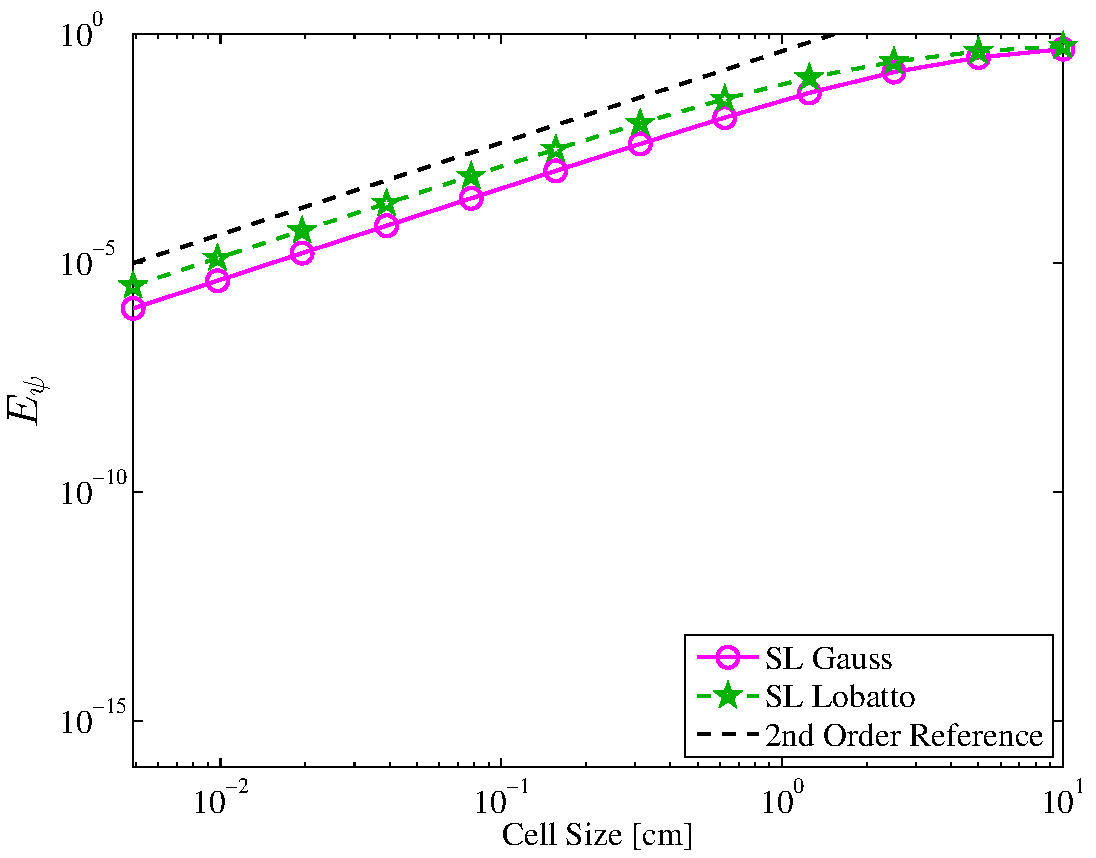
\includegraphics[width=11cm]{chapter2_constant_xs/Linear_L2_err-eps-converted-to.pdf}
\caption{Convergence rate of the $L_2$ norm of the error, $E_{\psi}$,  as a function of the mesh cell size for a pure absorber discretized with linear DFEM.}
\label{fig:multi_L2_p1}
\end{figure}
\begin{figure}[!htp]
\centering
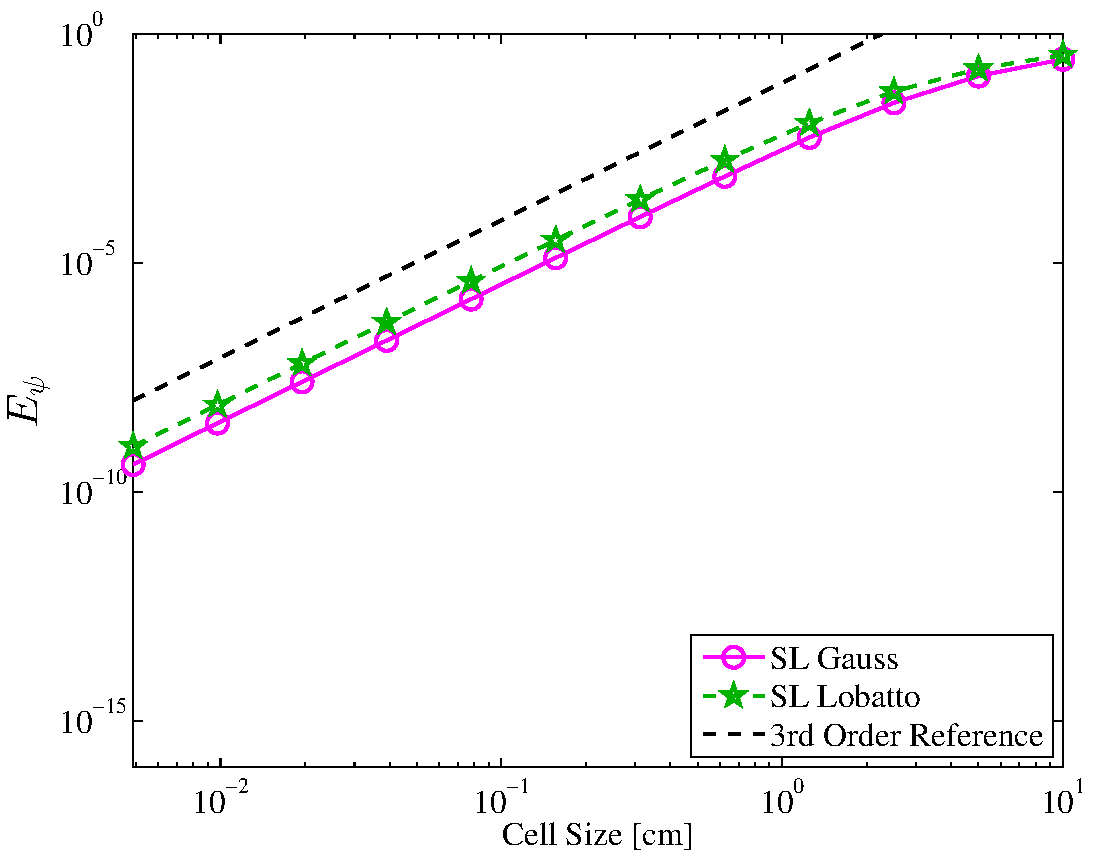
\includegraphics[width=11cm]{chapter2_constant_xs/Quadratic_L2_err-eps-converted-to.pdf}
\caption{Convergence rate of the $L_2$ norm of the error, $E_{\psi}$,  as a function of the mesh cell size for a pure absorber discretized with quadratic DFEM.}
\label{fig:multi_L2_p2}
\end{figure}
\begin{figure}[!hbp]
\centering
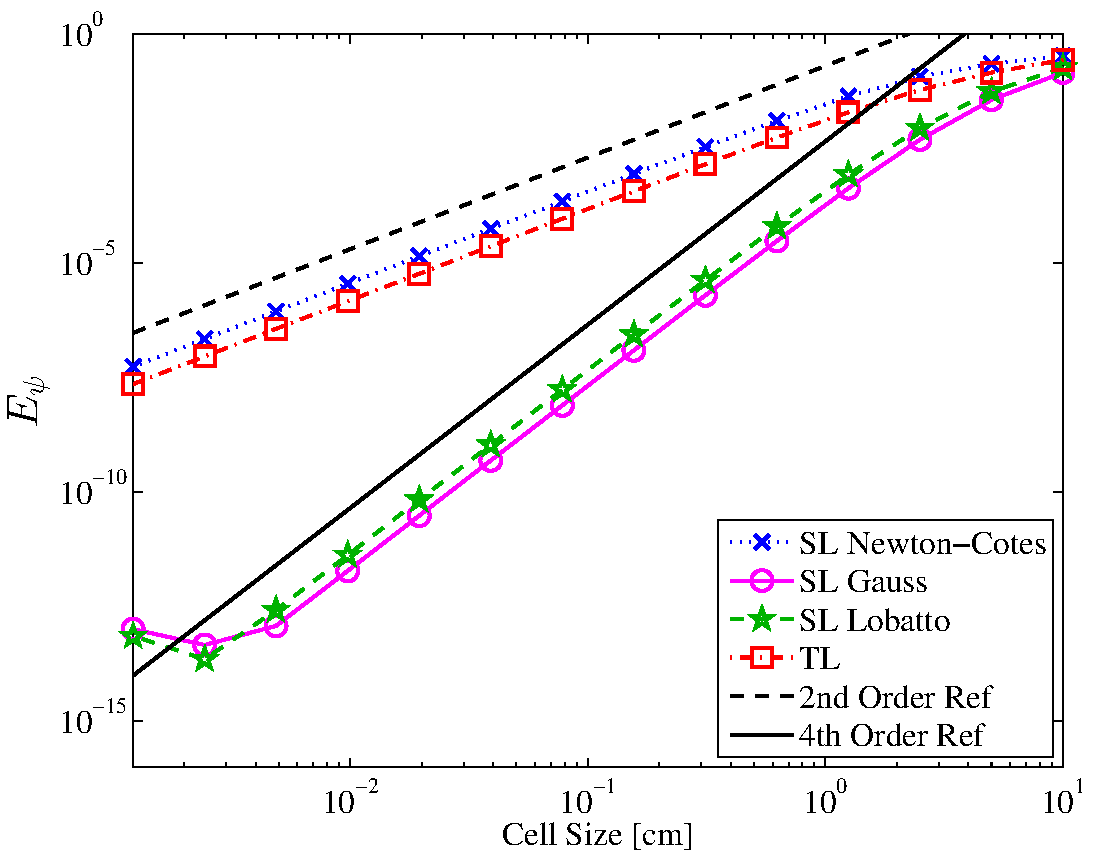
\includegraphics[width=11cm]{chapter2_constant_xs/Cubic_L2_err-eps-converted-to.pdf}
\caption{Convergence rate of the $L_2$ norm of the error, $E_{\psi}$,  as a function of the mesh cell size for a pure absorber discretized with cubic DFEM.}
\label{fig:multi_L2_p3}
\end{figure}
\begin{figure}[!htp]
\centering
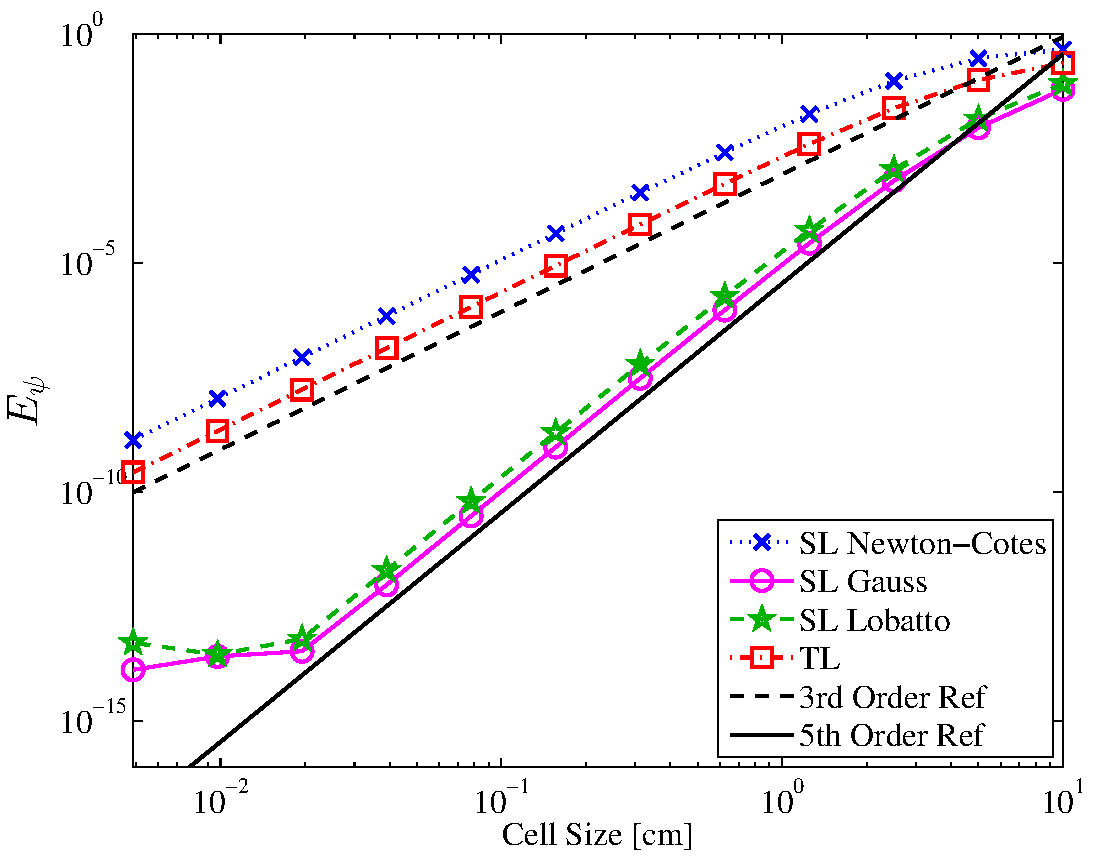
\includegraphics[width=11cm]{chapter2_constant_xs/Quartic_L2_err-eps-converted-to.pdf}
\caption{Convergence rate of the $L_2$ norm of the error, $E_{\psi}$,  as a function of the mesh cell size for a pure absorber discretized with quartic DFEM.}
\label{fig:multi_L2_p4}
\end{figure}
Figures \ref{fig:multi_L2_p1}-\ref{fig:multi_L2_p4} mirror the results of \tbl{tbl:taylor_in_part1} and \tbl{tbl:taylor_in_part2}, which is expected since the convergence rate of $E_{\psi}$ will be limited by the slowest converging local approximation which is $\widetilde{\psi}_{in,d}$.  
Similarly, \figs{fig:multi_L2A_p1}{fig:multi_L2A_p4} are the multiple-cell analogue of the local truncation error analysis of $\widetilde{\psi}_{A,d}$ given in \tbl{tbl:taylor_avg_part1} and \tbl{tbl:taylor_avg_part2}.  
\begin{figure}[!hbp]
\centering
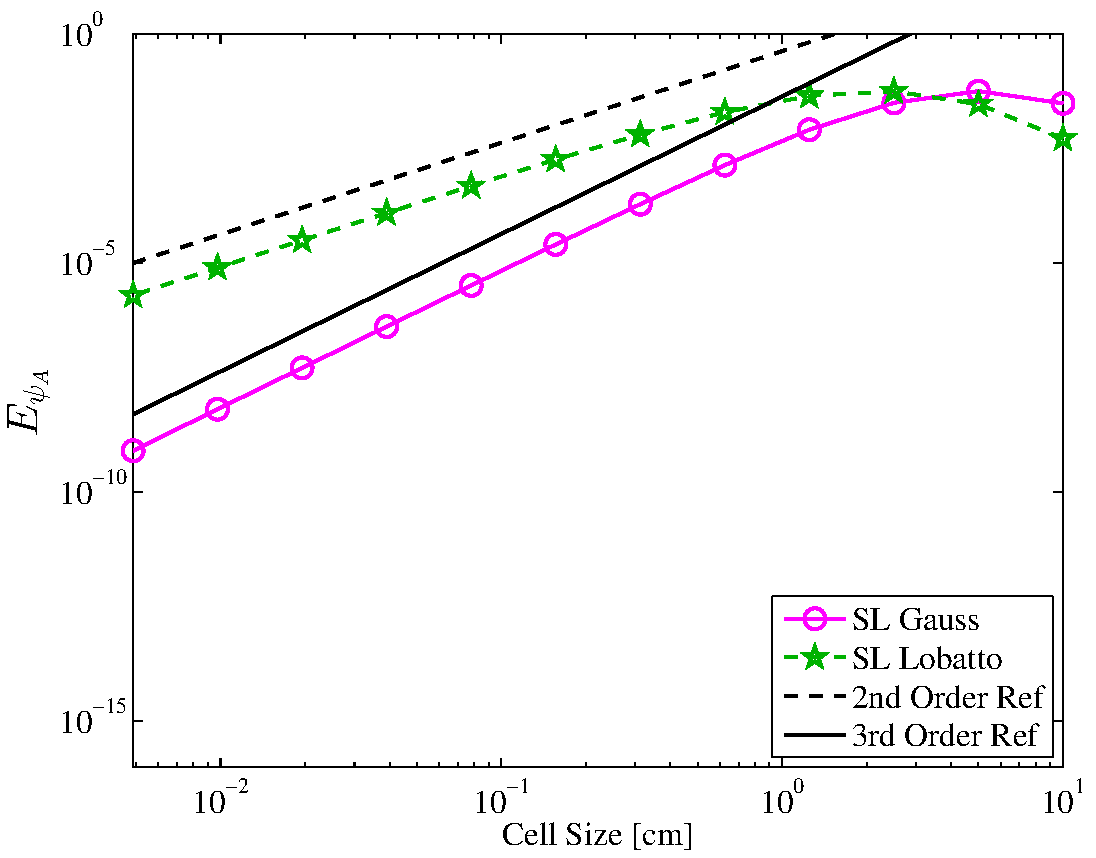
\includegraphics[width=11cm]{chapter2_constant_xs/Linear_L2A_err-eps-converted-to.pdf}
\caption{Convergence rate for $E_{\psi,A}$ as a function of the mesh cell size for a homogeneous pure absorber and linear DFEM.}
\label{fig:multi_L2A_p1}
\end{figure}
\begin{figure}[!htp]
\centering
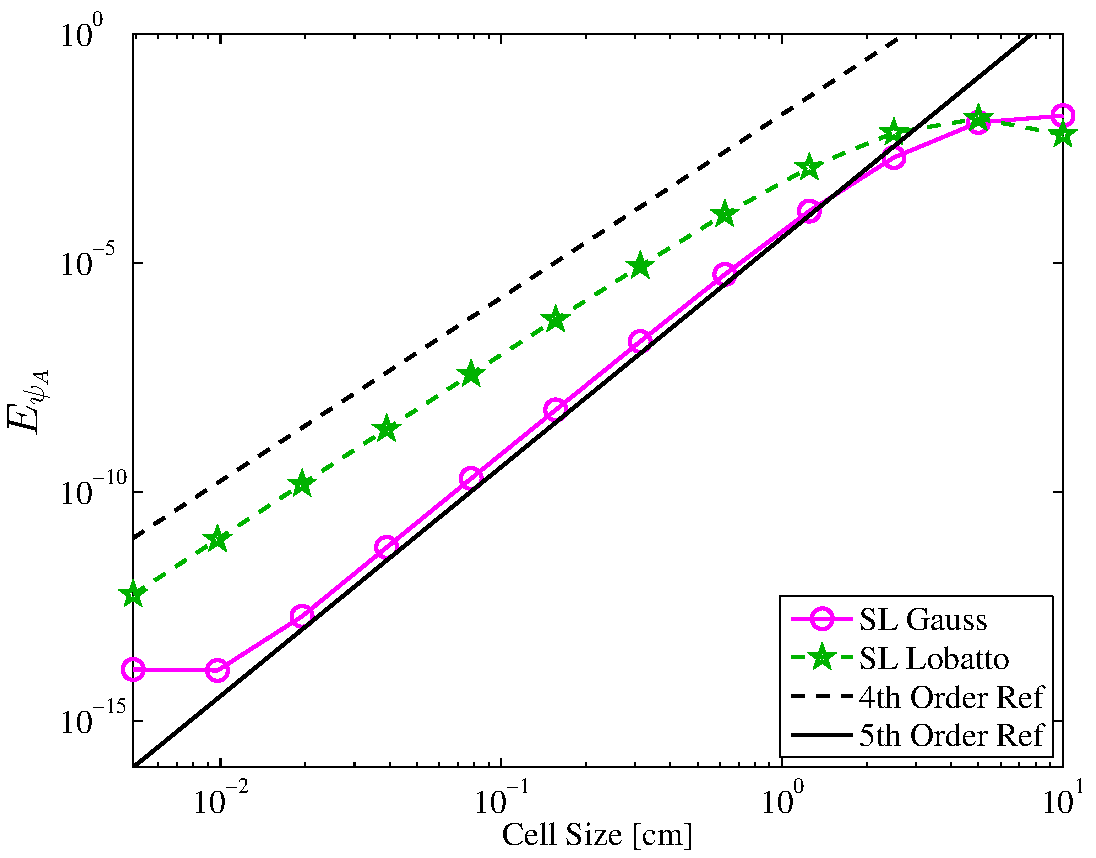
\includegraphics[width=11cm]{chapter2_constant_xs/Quadratic_L2A_err-eps-converted-to.pdf}
\caption{Convergence rate for $E_{\psi,A}$ as a function of the mesh cell size for a homogeneous pure absorber and quadratic DFEM.}
\label{fig:multi_L2A_p2}
\end{figure}
\begin{figure}[!hbp]
\centering
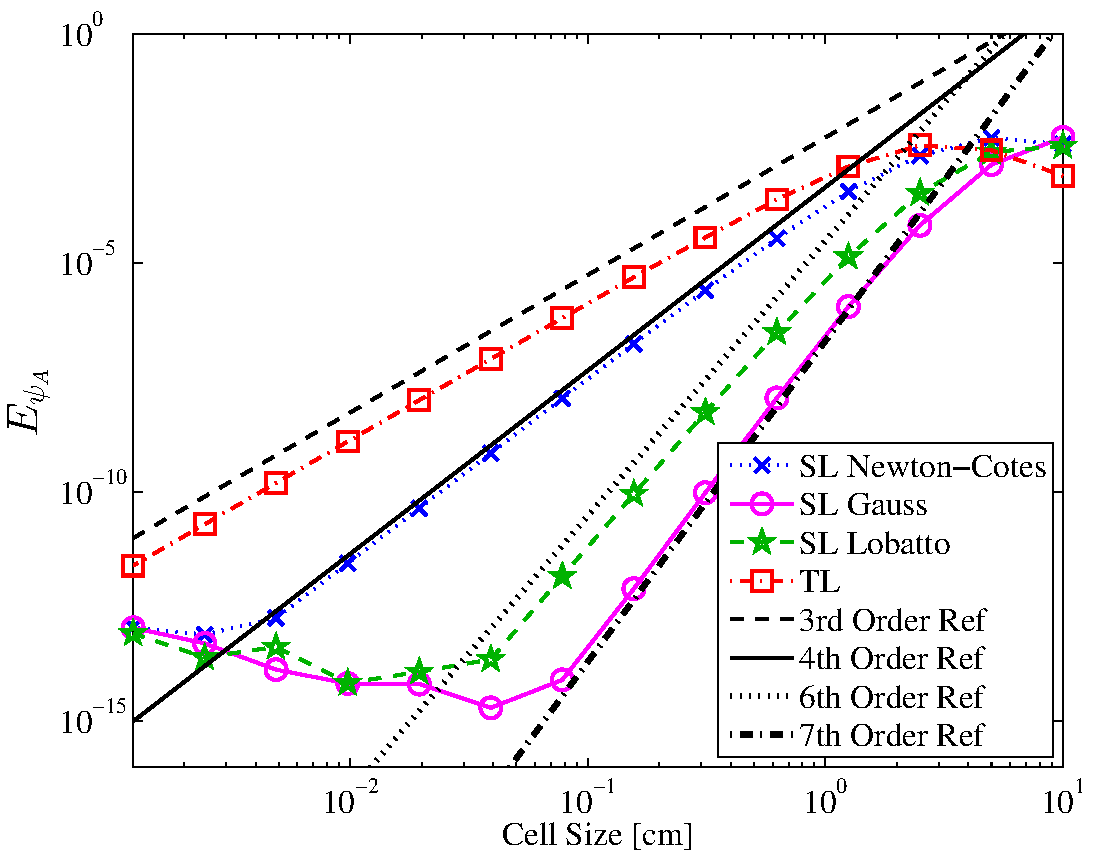
\includegraphics[width=11cm]{chapter2_constant_xs/Cubic_L2A_err-eps-converted-to.pdf}
\caption{Convergence rate for $E_{\psi,A}$ as a function of the mesh cell size for a homogeneous pure absorber and cubic DFEM.}
\label{fig:multi_L2A_p3}
\end{figure}
\begin{figure}[!htp]
\centering
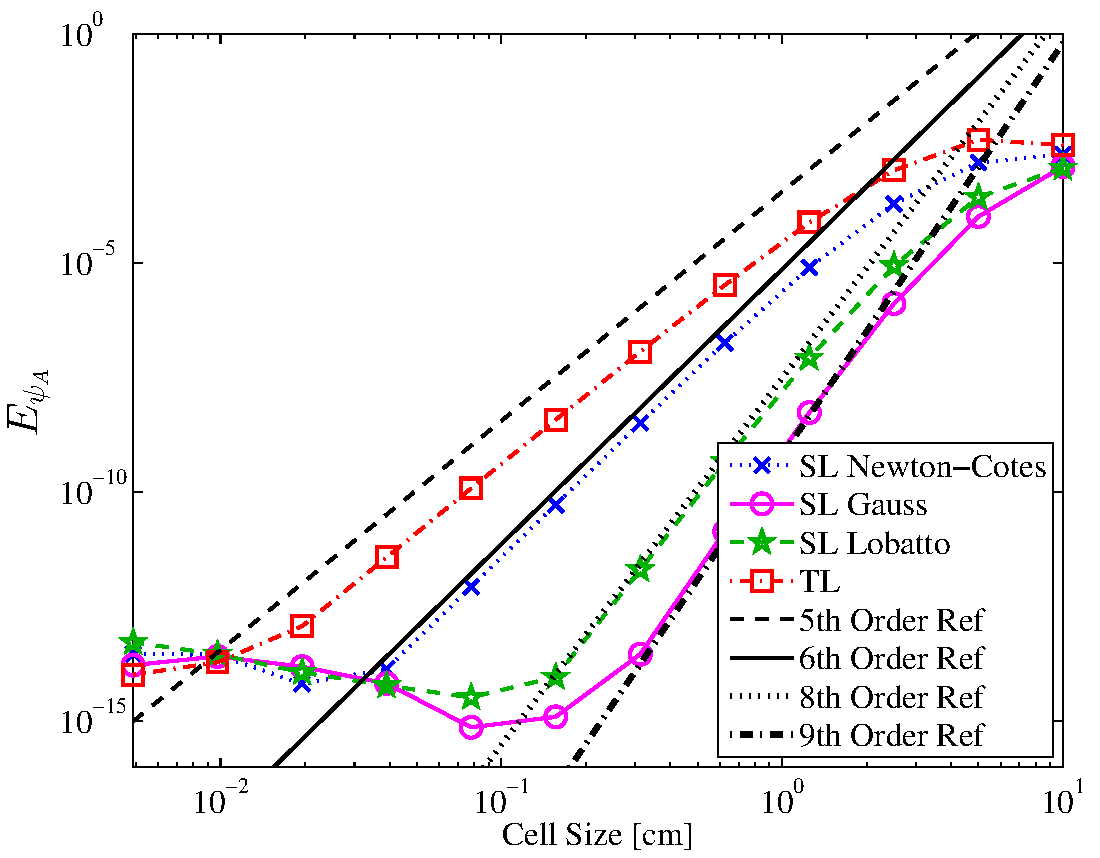
\includegraphics[width=11cm]{chapter2_constant_xs/Quartic_L2A_err-eps-converted-to.pdf}
\caption{Convergence rate for $E_{\psi,A}$ as a function of the mesh cell size for a homogeneous pure absorber and quartic DFEM.}
\label{fig:multi_L2A_p4}
\end{figure}
$E_{\psi_{out}}$, as shown in \figs{fig:multi_L2Out_p1}{fig:multi_L2Out_p4}, does not converge at the local truncation error rates of \tbl{tbl:taylor_out_part1} and \tbl{tbl:taylor_out_part2}.  
%

%
%
\begin{figure}[!hbp]
\centering
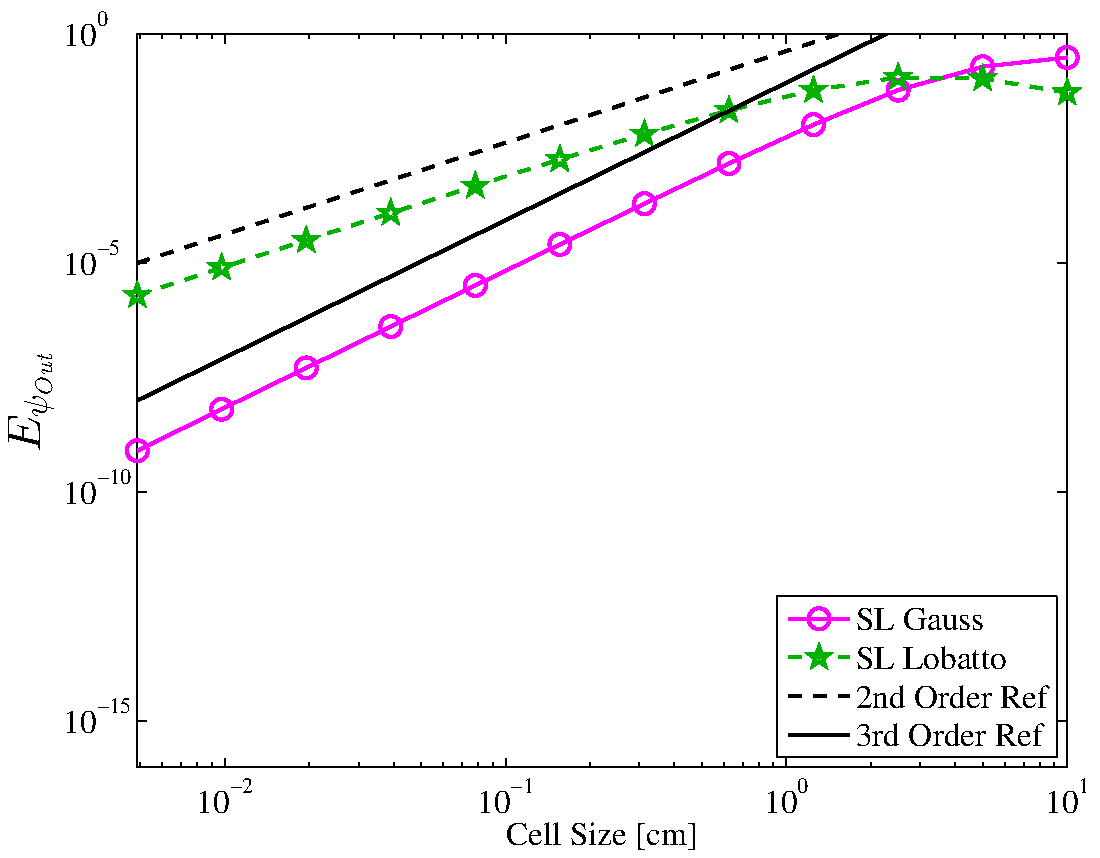
\includegraphics[width=11cm]{chapter2_constant_xs/Linear_L2Out_err-eps-converted-to.pdf}
\caption{Convergence rate of $E_{\psi,out}$ as a function of the mesh cell size for a homogeneous pure absorber for linear DFEM.}
\label{fig:multi_L2Out_p1}
\end{figure}
\begin{figure}[!htp]
\centering
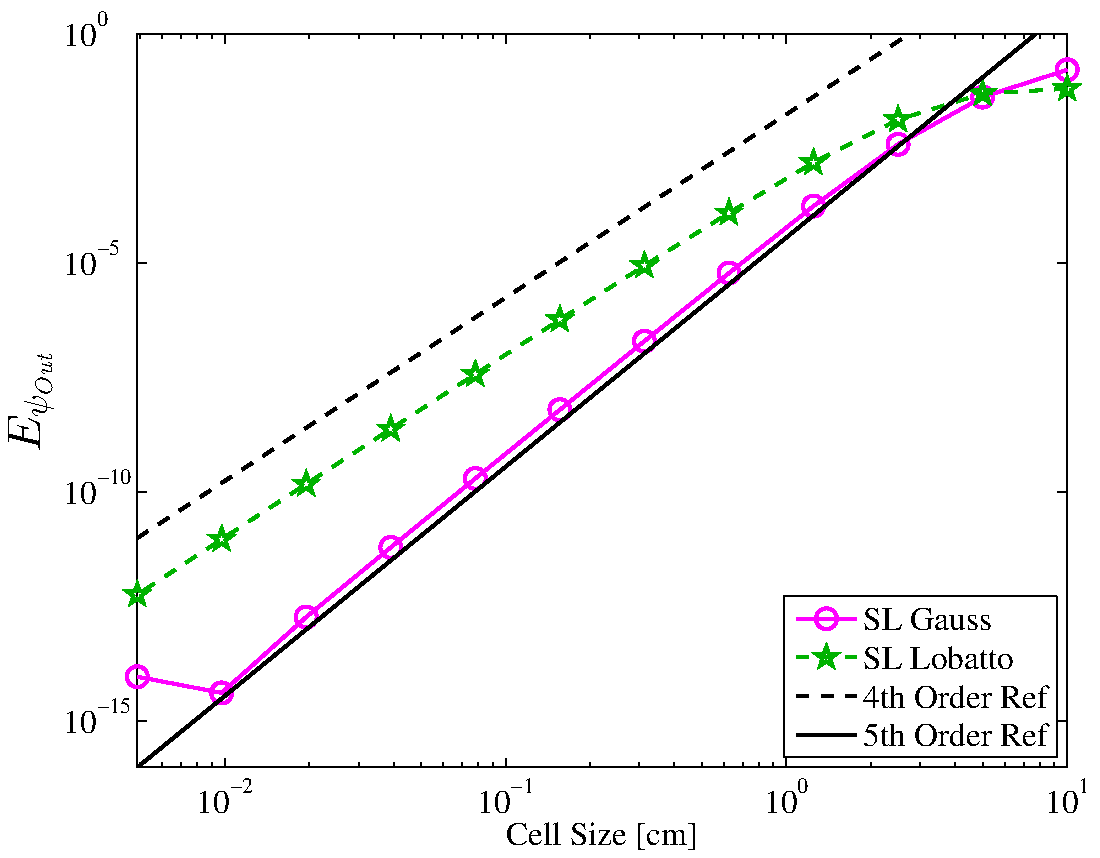
\includegraphics[width=11cm]{chapter2_constant_xs/Quadratic_L2Out_err-eps-converted-to.pdf}
\caption{Convergence rate of $E_{\psi,out}$ as a function of the mesh cell size for a homogeneous pure absorber for quadratic DFEM.}
\label{fig:multi_L2Out_p2}
\end{figure}
\begin{figure}[!hbp]
\centering
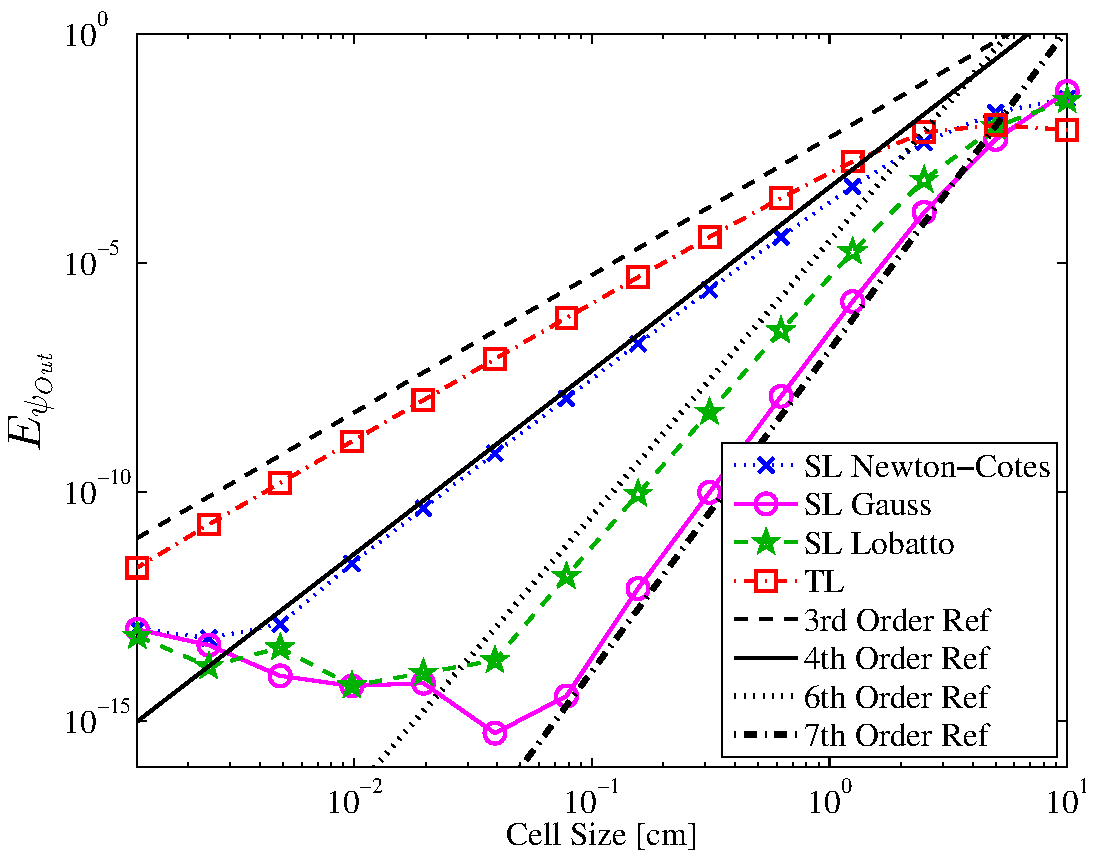
\includegraphics[width=11cm]{chapter2_constant_xs/Cubic_L2Out_err-eps-converted-to.pdf}
\caption{Convergence rate of $E_{\psi,out}$ as a function of the mesh cell size for a homogeneous pure absorber for cubic DFEM.}
\label{fig:multi_L2Out_p3}
\end{figure}
\begin{figure}[!htp]
\centering
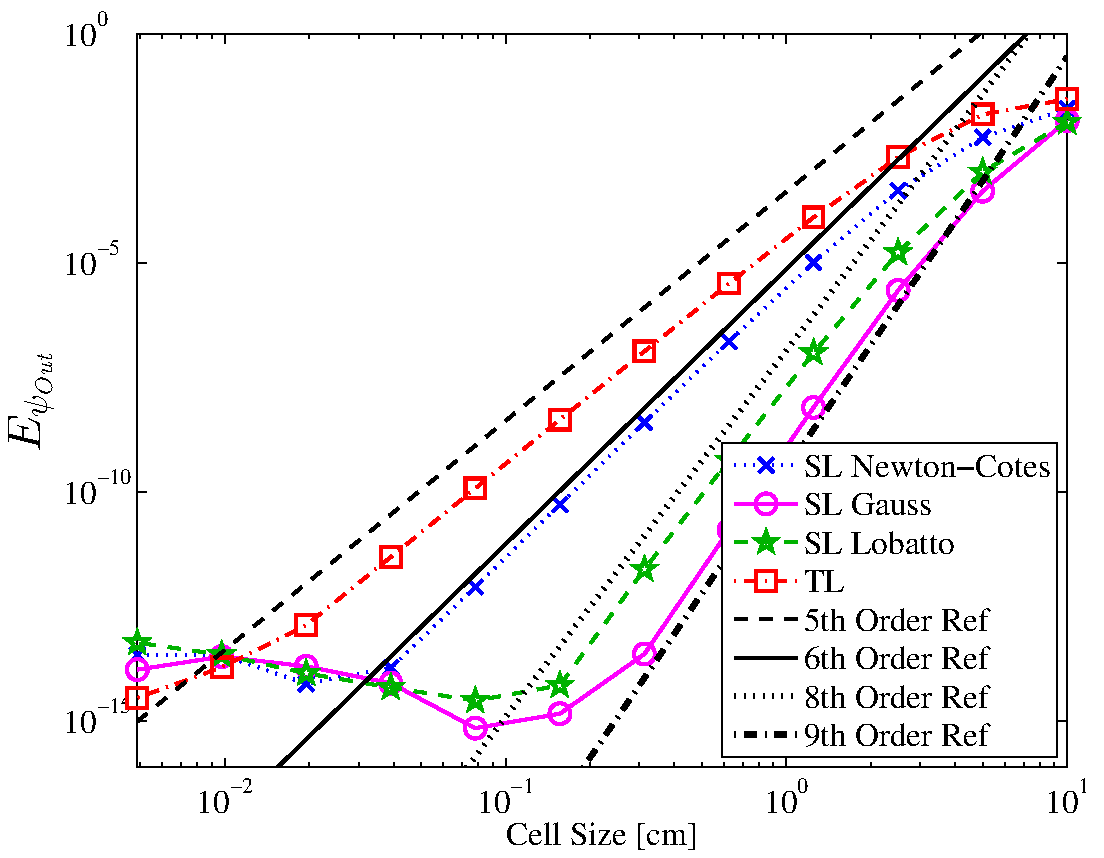
\includegraphics[width=11cm]{chapter2_constant_xs/Quartic_L2Out_err-eps-converted-to.pdf}
\caption{Convergence rate of $E_{\psi,out}$ as a function of the mesh cell size for a pure absorber for quartic DFEM.}
\label{fig:multi_L2Out_p4}
\end{figure}

\pagebreak
The accumulation of errors in multiple-cell problems causes $E_{\psi_{out}}$ to globally converge one order of accuracy lower than the local truncation orders given in \tbl{tbl:taylor_out_part1} and \tbl{tbl:taylor_out_part2}. 
It should be noted that the plateauing of errors $E_{\psi}$, $E_{\psi_A}$, and $E_{\psi_{out}}$ to values $\approx 10^{-14}$ 
in \figs{fig:multi_L2_p1}{fig:multi_L2_p4}, \figs{fig:multi_L2A_p1}{fig:multi_L2A_p4}, and \figs{fig:multi_L2Out_p1}{fig:multi_L2Out_p4}, respectively, is simply a result of our numerical solutions being limited by machine precision (double precision).

%%%%%%%%%%%%%%%%%%%%%%%%%%%%%%%%%%%%%%%%%%%%%%%%%%%%%%%%%%%%%%%%%%
%%%%%%%%%%%%%%%%%%%%%%%%%%%%%%%%%%%%%%%%%%%%%%%%%%%%%%%%%%%%%%%%%%
% \section{Conclusions}
% \label{sec:conclusions}
% %%%%%%%%%%%%%%%%%%%%%%%%%%%%%%%%%%%%%%%%%%%%%%%%%%%%%%%%%%%%%%%%%%
% %%%%%%%%%%%%%%%%%%%%%%%%%%%%%%%%%%%%%%%%%%%%%%%%%%%%%%%%%%%%%%%%%%
% %
% %\marginpar{\textcolor{red}{needs revisions}}
% %
% %\textcolor{red}{first recall what we did: sn transport, DFEM, higher order poly approx, mass lumping strategies}\\

% Lumping methods for arbitrary order DFEM spatial discretizations of the first-order form of the $S_N$ neutron transport equation have been studied in 1-D slab geometry.
% We have analyzed lumping in terms of numerical integration strategy and finite element basis function interpolation point type. Accuracy and robustness of the various
% schemes have been assessed.
% %
% %In particular, we have focused on analyzing numerical schemes (i.e., a combination of integration strategy and finite element basis function interpolation point type) that are both robust and accurate.  
% Robustness is defined in the traditionally accepted assertion in the radiation transport community, i.e., resistance to negative outflow angular flux solutions in source-free pure absorbers with incident angular flux as cell optical thickness is increased.
% Two forms of mass matrix lumping were studied in an attempt to find DFEM discretization schemes that are both robust and yield higher order accuracy with increases in the polynomial degree of the DFEM trial space.  

% The first scheme, traditional mass lumping or TL, exactly integrates the mass matrix and collapses row entries onto the main diagonal to create a diagonal mass matrix.  
% TL yields strictly positive angular flux outflows in a pure absorber with optically thick cells only when utilized with linear DFEM (LDFEM).
% The second form of mass matrix lumping considered here generates a diagonal mass matrix by restricting the DFEM interpolation points to the numerical quadrature points (this automatically generates a diagonal mass matrix).  
% This concept, termed self-lumping or SL, may be new to the radiation transport community but was already presented in \cite{raviart,thomee} in the general context of parabolic equations.
% We have extended these earlier works on self-lumping quadratures by using arbitrary degree polynomial trial spaces and studied three types of interpolation points: 
% (i) equally-spaced points, (ii) Gauss-Legendre quadrature, and (iii) Lobatto-Gauss-Legendre quadrature.  
% Using SL schemes, a strictly positive angular flux outflow can be obtained for all even degree polynomial trial spaces when employing Gauss-Legendre points (SL Gauss).  
% Positive outflow is also obtained for all odd degree polynomial trial spaces using either equally-spaced points (SL Newton-Cotes) or Lobatto-Gauss-Legendre quadratures (SL Lobatto).
% For source driven problems, regardless of mass matrix lumping scheme, it is still possible to obtain negative angular fluxes near cell inflows, for certain source distributions.
% %However, exact integration of fixed source moments will lead to a more robust scheme, regardless of mass matrix lumping strategy. % than if the source moments are approximately evaluated.


% In addition to the robustness of each scheme, we also considered the spatial convergence order of each method for a source-free purely absorbing medium with incident angular flux and constant cross section.  
% The most accurate mass matrix lumping scheme was SL Gauss, for which the average and outflow angular fluxes converged with an order $2P+1$, where $P$ is the polynomial degree of the trial space employed.  
% Since SL Gauss exactly integrates the mass matrix, its behavior is identical to employing exact DFEM, despite having a diagonal mass matrix.  TL was the least accurate of all schemes considered.  
% Increasing the degree of the finite element trial space did not guarantee increased convergence order when using the TL scheme.  
% The SL Newton-Cotes scheme performed better than TL; its order of convergence in the average and outflow angular fluxes increased with an increase in trial space polynomial degree, but in a suboptimal manner.  
% %Further, SL Newton-Cotes, like TL, was at most second order accurate for odd degree polynomial trial spaces and third order accurate for even degree trial spaces in approximating the cell inflow angular flux, respectively.  
% %This lack of local accuracy in calculating $\widetilde{\psi}_{in}$ translated to at most second order convergence for odd degree polynomial trial spaces and third order convergence for even degree polynomial trial spaces in 
% %the $L_2$-norm sense (that is, when calculating $E_{\psi}$).  
% Though not as accurate as SL Gauss for a given degree polynomial trial space, the SL Lobatto scheme only lagged SL Gauss' order of accuracy and spatial convergence by 1 for outflow and cell-averaged quantities.  
% %For all other quantities, SL Lobatto increased two orders of accuracy and spatial order of convergence for each increment in trial space degree, though was always one order less accurate than Exact DFEM and SL Gauss.

% In conclusion, we have shown that, for arbitrary degree polynomial trial space DFEM, a diagonal mass matrix does not necessarily ensure strictly positive angular flux outflow in a purely absorbing slab with spatially constant cross section.  
% Also, we have shown that by using quadrature-based lumping schemes and choosing DFEM interpolation points that are not equally spaced, robust, accurate polynomial DFEM schemes can be obtained.  
% Based on the observed robustness, accuracy, and spatial convergence order results, we conclude that, for applications requiring robust solution techniques, the SL Lobatto scheme with odd degree polynomial trial space DFEM 
% be used to discretize the angular flux .  
% If $p$-adaptivity is desired, software should be developed such that the ability to use either Lobatto (for odd trial space degrees) or Gauss (for even trial space degree) quadrature as the DFEM interpolation points is possible.  
% However, given the non-monotonic behavior of the outflow angular flux as a function of the cell optical thickness when employing the SL Gauss scheme with even degree trial spaces for under-resolved problems, using SL Lobatto 
% with an odd degree trial space would seem to be more accurate than using SL Gauss, despite SL Gauss being more accurate in the asymptotic (fine mesh) limit.

% We see additional opportunities for investigation. % before self-lumping schemes can be used in high order accuracy radiative transfer calculations.
% In particular, we plan on examining the robustness and accuracy of self-lumping DFEM schemes for situations where the cross section is not cell-wise constant.  
% In radiative transfer, the opacity (analog of a cross section) strongly depends on temperature, with temperature varying also within each mesh cell. Thus, opacity is an arbitrary, possibly rapidly, varying function of space.
% The behavior of self-lumping DFEM schemes when cross section is a continuously varying function of space will be of interest in radiative transfer calculations and, as such, should be considered as a topic of research on that subject.

% We also see opportunities to apply self-lumping quadrature to multi-dimensional geometries.  
% While we do not anticipate the multi-dimensional extensions of SL Lobatto or SL Gauss schemes to yield strictly positive angular flux outflows in multi-dimensional geometries, the mass matrix self-lumping technique we have examined here 
% in slab geometry provides a framework not only for mass matrix lumping but also for gradient matrix lumping.
% % in multidimensional geometries.  
% In multi-dimensional problems, mass matrix lumping alone has been shown to be insufficient in preventing solution oscillations. 
% To reduce these oscillations, gradient operator lumping is also required \cite{adams}.
% Though gradient lumping is straightforward on orthogonal grids, it is an open topic of research for non-orthogonal grids \cite{morel_lump}.  Self-lumping methods may provide an adequate framework 
% to carry out consistent mass and gradient lumping on non-orthogonal meshes.

